\documentclass[11pt,a4paper]{article}
\usepackage[a4paper,margin=25mm]{geometry}
\usepackage[T1]{fontenc}
\usepackage{xcolor,tikz,float}
\usetikzlibrary{calc}
\definecolor{glowblue}{HTML}{24576C}
\definecolor{glowgold}{HTML}{BE771E}
\usepackage{lmodern,microtype,amsmath,amssymb,amsthm,booktabs}
\usepackage[colorlinks=true,linkcolor=black,citecolor=magenta,urlcolor=black]{hyperref}
\urlstyle{same}
\newtheorem{thm}{Theorem}[section]
\newtheorem{introthm}{Theorem}
\renewcommand{\theintrothm}{\Alph{introthm}}
\newtheorem{prop}[thm]{Proposition}
\newtheorem{lem}[thm]{Lemma}
\newtheorem{cor}[thm]{Corollary}
\newtheorem{defn}[thm]{Definition}
\newtheorem{question}[thm]{Question}
\newtheorem{conjecture}[thm]{Conjecture}
\theoremstyle{remark}
\newtheorem{rem}[thm]{Remark}
\setlength{\parskip}{1pt}\setlength{\emergencystretch}{2em}
\raggedbottom
\setcounter{tocdepth}{1}
\setcounter{MaxMatrixCols}{20}
\title{Planar rotators with Hadamard couplings}
\author{Chat, Opus and Teo}
\date{}
\hypersetup{pdftitle={Planar rotators with Hadamard couplings},pdfauthor={Chat, Opus and Teo}}
\begin{document}
\maketitle
\begin{abstract}
A complex Hadamard matrix $H$ of order $N$ can be read as a magnetic flux pattern on an array of $2N$ crossed superconducting wires, coupled by Josephson junctions, the Fourier matrix corresponding to the uniform field of Chandra, Ioffe and Sherrington. The glow of $H$, the law of $\langle Hb,a\rangle$ for random phase vectors $a,b$, determines the energy distribution of this system of planar rotators by real projection. We prove moment polynomiality for elementary abelian Fourier matrices, including Walsh matrices, and compute the moments through order 12 for all complex Hadamard matrices, in terms of flux harmonics. The leading high-temperature expansion of the pressure has universal Catalan coefficients, as for Haar unitary couplings. The ground states correspond to bistochastic forms with positive line sums, and we compute the edge asymptotics for $W_2,W_4$. With Villain bonds between neighboring wires and the junction coupling switched off, the Fourier 4th moment crosses over at correlation length $\sqrt N$.
\end{abstract}
\begingroup
\color{magenta}\hypersetup{linkcolor=magenta}
\setlength{\parskip}{0pt}
\makeatletter
\renewcommand{\l@section}[2]{%
 \ifnum\c@tocdepth>\z@
 \addpenalty{\@secpenalty}
 \addvspace{1pt}
 \setlength\@tempdima{1.8em}
 \begingroup
 \parindent\z@ \rightskip\@pnumwidth
 \parfillskip-\@pnumwidth
 \leavevmode\bfseries
 \advance\leftskip\@tempdima \hskip-\leftskip
 #1\nobreak\hfil\nobreak\hb@xt@\@pnumwidth{\hss #2}\par
 \endgroup
 \fi}
\makeatother
\tableofcontents
\endgroup

\section*{Introduction}
\phantomsection\addcontentsline{toc}{section}{Introduction}
This paper starts with a game and ends with some physics. The game was invented for fun, independently, by Gale and Berlekamp, and Berlekamp built a board of it for the common room at Bell Labs. A square board carries a lamp at each intersection of its rows and columns, and every row and every column has a switch, reversing all the lamps on it. Starting from some pattern of lit lamps, the player throws switches and tries to make the board as bright, or as dark, as possible. With $H_{jk}=\pm1$ recording the lamps and $a_j,b_k=\pm1$ the switches, the score is the sum of the entries of the switched board,
\[
 \Omega=\sum_{jk}H_{jk}a_jb_k
\]
The complex version replaces the signs by phases. For a matrix $H\in M_N(\mathbb T)$ and phase vectors $a,b\in\mathbb T^N$, put
\[
 \Omega_H=\langle Hb,a\rangle=\sum_{jk}H_{jk}\bar a_jb_k
\]
where we use scalar products linear on the left, $\langle x,y\rangle=\sum_jx_j\bar y_j$. When $H$ is a complex Hadamard matrix, meaning that its rows are pairwise orthogonal, and $a,b$ are independent and uniform, the law of $\Omega_H$ is called the glow of $H$ \cite{banica}. It is invariant under Hadamard equivalence. The normalized glow is the law of $Z_H=\Omega_H/N$. We have $E(|Z_H|^2)=1$, and as $N$ grows the law of $Z_H$ approaches the standard complex Gaussian law \cite{banica}. The higher moments record information about $H$.

The real part of the same sum gives the energy of a physical system. Take 2 layers of $N$ parallel superconducting wires, the wires of one layer crossing those of the other at right angles, and put a Josephson junction at each of the $N^2$ crossings. Each wire carries a single superconducting phase, $a_j$ for the $j$th row wire and $b_k$ for the $k$th column wire, and the junction at the crossing $jk$ has energy
\[
 -E_J\,Re\big(H_{jk}\bar a_jb_k\big)
\]
where the phase factor $H_{jk}$ records the magnetic vector potential. Chandra, Ioffe and Sherrington proposed this array to study glassy behavior without disorder \cite{cis}. A uniform flux $\Phi_0/N$ per cell, with $\Phi_0$ the flux quantum, gives the Fourier matrix $F_N=(e^{2\pi ijk/N})$. In the ideal array one can prescribe the $(N-1)^2$ cell fluxes independently. They determine $H$ up to row and column phases, and Hadamard equivalence also allows renaming the wires. The normalized density of states is the distribution of $-E_J\,Re(\Omega_H)$ under uniform phases. Its moments give the high-temperature expansion. Its lower edge is attained at bistochastic forms with positive line sums.

There is a second motivation. The question of the statistical mechanical meaning of Hadamard matrices was raised by Jones, and has accompanied the theory of subfactors since its beginnings \cite{jo1}. In Jones' spin models \cite{jo2}, the invariance under the 2nd Reidemeister move asks for a matrix $W$ with $\sum_xW_{ax}/W_{bx}=N\delta_{ab}$, which for entries of modulus 1 is exactly the Hadamard condition. The associated subfactors and planar algebras \cite{jo3,jo4} give one answer, and their invariants are a subject of current computations \cite{abf}. The array above gives another beginning of an answer, with the matrix entering as a magnetic field, and with the Hadamard condition saying that the coupling matrix $H/\sqrt N$ is unitary.

We study the array at all temperatures that are accessible to exact calculation. At high temperature the moments of the glow are polynomial in the order, for the Fourier matrices of elementary abelian groups. The moment expansion uses the coefficients of $\log f(t)$, with $f(t)=\sum_{m\ge0}t^m/m!^2$, and for these matrices the remaining terms count solutions of finite linear systems.

\begin{samepage}
\begin{introthm}\label{intro:poly}
For every prime $q$ and every $p\ge1$, there is a polynomial $P^{(q)}_p$ of degree $2p$ such that
\[
 E\left(|\Omega_{F_{\mathbb Z_q^n}}|^{2p}\right)=P^{(q)}_p(q^n)
\]
for all $n\ge0$. For each fixed $p$, these polynomials stabilize to a polynomial $P^\infty_p$ when $q$ is sufficiently large. In particular the glow moments of the Walsh matrices are polynomial in their size.
\end{introthm}
\end{samepage}

This proves the Walsh polynomiality conjecture of \cite{banica}. We compute the polynomials through $p=8$ in the Walsh and generic cases. Their differences record the characteristic of the group. At a fixed small $N$, the evaluations $P^\infty_p(N)$ can fail the positivity conditions for moments; Section~\ref{sec:walsh} gives an explicit obstruction at $N=2$.

For general Hadamard matrices, the first deviations are governed by entrywise powers. Put
\[
 S_k(H)=\|H^{\circ k}(H^{\circ k})^*-N1_N\|^2
\]
with the Hilbert--Schmidt norm. In the array, if $\Phi$ is a rectangle's flux in units of the flux quantum, then
\[
 S_k(H)=N^2(N-1)+4\sum_{a<b,\ j<l}\cos\big(2\pi k\Phi(a,b;j,l)\big)
\]
The sum uses each rectangle with distinct sides once. At $p=6$, 2 cubic contractions occur as well, built on 3 row wires and 3 column wires. They are formed from
\[
 B=H^{\circ2}(H^{\circ2})^*-N1_N,\qquad
 Q_{abc}=\sum_j H_{aj}^2\bar H_{bj}\bar H_{cj}
\]
and take the form $R(H)=Tr(B^3)$ and
$T(H)=Re\sum_{abc\ {\rm distinct}}Q_{abc}Q_{bca}Q_{cab}$, with ordered triples. These are invariants of Hadamard equivalence and transposition.

\begin{samepage}
\begin{introthm}\label{intro:moments}
For independent uniform phases, the moments of a complex Hadamard matrix satisfy
\[
 E(|\Omega_H|^{2p})=P^\infty_p(N)\qquad(p\le3)
\]
and
\[
\begin{gathered}
 E(|\Omega_H|^8)=P^\infty_4(N)+18S_2(H)\\[5pt]
 E(|\Omega_H|^{10})=P^\infty_5(N)+(450N^2-3600N+9600)S_2(H)\\[5pt]
 E(|\Omega_H|^{12})=P^\infty_6(N)+A(N)S_2(H)+51200S_3(H)+2700R(H)+21600T(H)
\end{gathered}
\]
where $A(N)=8100N^4-137700N^3+1062450N^2-4436100N+7663500$, and $R,T$ are the cubic contractions above.
\end{introthm}
\end{samepage}

The 8th and 10th moments attain their upper bounds exactly at matrices equivalent to real Hadamard matrices, which are the flux patterns with 0 or half a flux quantum through each cell. At the 12th moment, the Tao matrix lies below the generic polynomial value, while the family $H_6^{e^{it}}$ has constant moments through $p=5$ and a 12th moment varying with $\cos(4t)$.

The logarithm of the moment generating function gives the pressure after rescaling. At every fixed order of its high-temperature expansion the leading coefficient is universal and agrees with the Haar unitary calculation. This is the rigorous counterpart, for our arrays, of the observation of Marinari, Parisi and Ritort that deterministic spin glasses with orthogonal couplings have the high-temperature expansion of random orthogonal couplings \cite{mp1,mp2,ppo}.

\begin{samepage}
\begin{introthm}\label{intro:free}
Let $H$ be a complex Hadamard matrix of order $N$. For independent
uniform phase vectors $a,b$, put $\Omega_H=\langle Hb,a\rangle$ and
\[
 G_H(t)=\sum_{k\geq0}\frac{E(|\Omega_H|^{2k})}{(k!)^2}\,t^k
\]
Then we have
\[
 \frac{1}{N}\log G_H(x/N)\ \longrightarrow\
 \sqrt{1+4x}-1-\log\frac{1+\sqrt{1+4x}}2
\]
coefficientwise as $N\to\infty$, uniformly in $H$ at each fixed order.
For $H=F_{\mathbb Z_q^n}$ the term of order one in $\log G_H(x/N)$ is
the same formal series for all odd primes $q$.
\end{introthm}
\end{samepage}

At inverse temperature $\beta$ the variable $x$ is $\beta^2/4$. The formula predicts that the mean energy, divided by its ground state value, is $m(\beta)=\beta/(1+\sqrt{1+\beta^2})$, increasing from 0 at infinite temperature to 1 at zero temperature. Whether the equilibrium formula holds at fixed temperature is open, even at the Fourier point. The dynamical glass instability studied in \cite{cfi,cis} concerns a different, weak-field regime.

At zero temperature and fixed $N$, the geometry of the ground states takes over. Their existence for every $H$ is the Idel--Wolf theorem \cite{iwo}, and for the Fourier arrays explicit examples come from the Chu sequences of radar and telecommunication engineering \cite{chu,fza}. The normalized moments $M_p(H)=E[(|\Omega_H|^2/N^3)^p]$ decay at a rate which depends on how these ground states meet.

\begin{samepage}
\begin{introthm}\label{intro:edge}
For the 2 smallest nontrivial Walsh matrices, we have
\[
 M_p(W_2)\sim\frac{2}{\pi p},\qquad
 M_p(W_4)\sim\frac{2\sqrt2\,\Gamma(1/4)^3}{\pi^{9/2}}\,p^{-9/4}
\]
as $p\to\infty$. For $W_4$ the leading term comes from the crossings of 3 families of ground states.
\end{introthm}
\end{samepage}

The last part of the paper lets the neighboring wires interact. Arrange the row wires, and the column wires, around a cylinder, and couple neighboring parallel wires by Villain bonds \cite{villain}. At zero coupling between the 2 layers, $a$ and $b$ are then independent periodic Villain chains. The parameter $l$ is fixed by the infinite-chain correlation $e^{-|r|/l}$. At $l=0$ the phases are independent and one recovers the glow. At fixed $N$, increasing $l$ aligns the phases within each layer. In the limit $Z$ is the normalized entry sum of the chosen representative times a uniform phase. The transfer operator of the chain has Fourier eigenvalues $e^{-n^2/l}$, which allow exact finite-size calculations. For the Fourier array, translation invariance selects the 4 sites $0,x,y,x+y$ in the 4th-moment expansion, and the Villain expectation on this parallelogram is $e^{-2\min(|x|_N,|y|_N)/l}$.

\begin{samepage}
\begin{introthm}\label{intro:fourier}
For 2 independent periodic Villain chains, put $Z_N=N^{-1}\langle F_Nb,a\rangle$. We have $E(|Z_N|^2)=1$ for every $N$ and every correlation length. Let $N\to\infty$ and choose the correlation length $l=l_N$. If $l_N\sim c\sqrt N$ for a fixed $c>0$, then
\[
 \lim_{N\to\infty}E(|Z_N|^4)=M(c)
\]
where
\[
 M(c)=1+E\left[
 \left(1-\frac2\pi\, Si\left(\frac{\pi c^2}{2}\,UV\right)\right)^2\right]
\]
with $U,V$ independent exponential variables of mean 1 and $Si(t)=\int_0^t\sin(v)\,dv/v$. The function $M$ decreases strictly from $2$ to $1$ as $c$ increases from $0$ to $\infty$. If instead $l_N/\sqrt N\to\infty$, the law of $Z_N$ converges to uniform measure on the unit circle as $N\to\infty$.
\end{introthm}
\end{samepage}

Thus the modulus of the Fourier sum becomes asymptotically constant already on a scale where distant wires may remain weakly correlated. Here $l_N\sim c\sqrt N$ means $l_N/(c\sqrt N)\to1$. For a general matrix the cyclic labeling matters, and rephasing changes the excess, the sum of the entries, which determines the fully aligned limit. Write $C=E(aa^*)=E(bb^*)$ for the correlation matrix of a Villain chain.

\begin{samepage}
\begin{introthm}\label{intro:general}
For a complex Hadamard matrix $H$ with cyclically labeled rows and columns, put $Z_l=\langle Hb,a\rangle/N$, where $a,b$ are independent periodic Villain chains of correlation length $l$. Then
\[
 E(|Z_l|^2)=\frac1{N^2}\,Tr(CHCH^*)
\]
and, at fixed $N$,
\[
 \lim_{l\to\infty}Z_l=\frac{u}{N}\,\sum_{jk}H_{jk}
\]
where the limit is understood in law and $u$ is uniform on $\mathbb T$. The radius of this limiting law is at most $\sqrt N$, with equality exactly when all row and column sums of $H$ are the same number of modulus $\sqrt N$.
\end{introthm}
\end{samepage}

A common phase makes the line sums of each equality case positive and gives a ground state of the array. Figure~\ref{fig:map} in Section~\ref{sec:glow} places all these results on a map whose 2 coordinates are the inverse temperature and the stiffness $l$. Sections~\ref{sec:moments}--\ref{sec:edge} go from high temperature to zero temperature, and Sections~\ref{sec:villain}--\ref{sec:general} switch on the stiffness.

\medskip {\em Acknowledgements.} We would like to thank Paul Dario for useful discussions.

\section{Planar rotators and Josephson arrays}\label{sec:glow}

We first recall the switching game and the glow, and then explain how the glow describes an array of superconducting wires coupled by Josephson junctions.

\medskip

\noindent\textbf{Phases and Fourier matrices.} 
A phase is a point of the unit circle $\mathbb T=\{z\in\mathbb C:|z|=1\}$. A uniform
phase is $u=e^{it}$ with $t$ uniform on $[0,2\pi)$. Its basic integration
rule is
\[
 E(u^p\bar u^{\,q})=\int_0^{2\pi}e^{i(p-q)t}\frac{dt}{2\pi}
 =\delta_{pq},\qquad p,q\geq 0
\]
Here $\delta_{pq}$ is 1 when $p=q$ and 0 otherwise. The finite version is just as useful. Write $G=\mathbb Z_N$, choose
$w=e^{2\pi i/N}$, and index rows and columns from $0$ to $N-1$. Then
\[
  \sum_{j\in G}w^{jh}=N\delta_{h0}
\]
Here $\delta_{h0}$ refers to equality in $G$. For $h\ne 0$ this is the sum of a geometric progression. Thus the matrix
$F=(w^{jk})_{j,k\in G}$ satisfies $FF^*=NI$, where $*$ is the conjugate
transpose. We use the unnormalized Fourier matrix throughout.

More generally, a complex Hadamard matrix is a square matrix $H$ whose
entries have modulus 1 and for which $HH^*=NI$. Multiplying the rows
and columns by phases preserves both properties. The sum of the entries
after such a change is
\[
   \langle Hb,a\rangle=\sum_{jk}H_{jk}\bar a_jb_k
\]
This is the scalar product of $Hb$ with $a$, with our convention of linearity on the left.

\medskip
\noindent\textbf{The switching game.}
Imagine a square city with a lamp at each intersection and a master switch on
each street. Each switch reverses every lamp on its row or column.
David Gale and Elwyn Berlekamp devised the game independently \cite{kas}.
Berlekamp built a board with 100 bulbs that stood in the mathematics
common room at Bell Labs in Murray Hill \cite{slo}. A challenger set the puzzle
with 100 switches on the back. The player had just 20 switches on the front
and tried to leave as few bulbs lit as possible. A photograph of the board
appears in \cite[Plate~1]{fsl}. Flipping all row switches complements the board,
so one can equally well play for the brightest city.
Figure~\ref{fig:lamps} shows one move on the order-4 Hadamard board of \cite{banica}.

\begin{figure}[htb!]
\centering
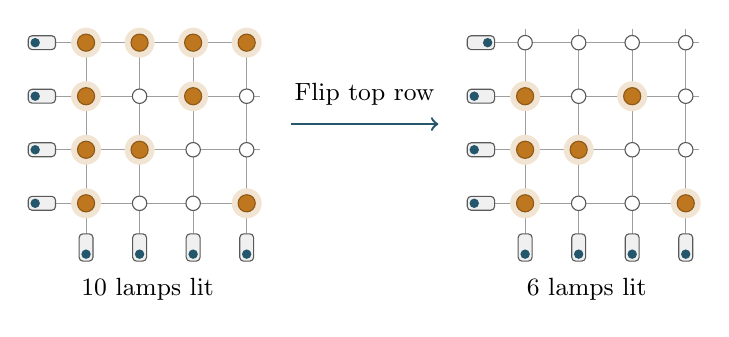
\begin{tikzpicture}[x=6.8mm,y=6.8mm,font=\small]
  \foreach \shift/\after/\countlit in {0/0/10,8.2/1/6}{
    \begin{scope}[shift={(\shift,0)}]
      % Rows are listed from the top, as on the switching board.
      \foreach \y in {0,...,3}{
        \draw[black!38] (-.57,\y)--(3.25,\y);
        \pgfmathtruncatemacro{\flipped}{(\y==3 && \after==1)}
        \draw[rounded corners=1.4pt,fill=black!6,draw=black!65]
          (-1.08,\y-.13) rectangle (-.57,\y+.13);
        \fill[glowblue] ({-.95+.25*\flipped},\y) circle[radius=.088];
      }
      \foreach \x in {0,...,3}{
        \draw[black!38] (\x,-.57)--(\x,3.25);
        \draw[rounded corners=1.4pt,fill=black!6,draw=black!65]
          (\x-.13,-1.08) rectangle (\x+.13,-.57);
        \fill[glowblue] (\x,-.95) circle[radius=.088];
      }
      \foreach \row [count=\i from 0] in {{1,1,1,1},{1,0,1,0},{1,1,0,0},{1,0,0,1}}{
        \foreach \lamp [count=\j from 0] in \row{
          \pgfmathtruncatemacro{\lit}{mod(\lamp+(\i==0)*\after,2)}
          \ifnum\lit=1
            \fill[glowgold!20] (\j,3-\i) circle[radius=.28];
            \filldraw[draw=glowgold!75!black,fill=glowgold]
              (\j,3-\i) circle[radius=.16];
          \else
            \draw[draw=black!65,fill=white] (\j,3-\i) circle[radius=.135];
          \fi
        }
      }
      \node at (1.15,-1.60) {\countlit\ lamps lit};
    \end{scope}
  }
  \draw[->,line width=.85pt,glowblue] (3.82,1.48)--(6.58,1.48)
    node[midway,above=3pt,text=black] {Flip top row};
\end{tikzpicture}
\caption{Each filled disc is a lit lamp. Throwing one switch turns off the
four lamps in the top row.}\label{fig:lamps}
\end{figure}

Write $H_{jk}=1$ for a lit lamp and $H_{jk}=-1$ for a dark one.
Row and column switches multiply these signs by $a_j,b_k\in\{1,-1\}$,
so $\langle Hb,a\rangle$ counts lit lamps minus dark lamps.
In coding terms the boards reachable from an all-dark board form a binary linear code.
The player's minimum is the Hamming distance from the initial board to that
code \cite{rvi}. Choosing the switches independently at random gives the
law of the imbalance.
For the complex glow we make the same experiment with uniform phases on
$\mathbb T$ in place of random signs.

\begin{samepage}
\begin{defn}
For a complex Hadamard matrix $H$ of order $N$, choose the $2N$ entries of
$a,b$ independently and uniformly on $\mathbb T$. The \emph{glow} of $H$ is the law
of $\langle Hb,a\rangle$. We call the law of $Z=\langle Hb,a\rangle/N$ its normalized glow.
\end{defn}
\end{samepage}

For a catalogue of complex Hadamard matrices organized by equivalence
class, see \cite{tzy}. If $H$ is changed by deterministic row or column phases or permutations,
the independent uniform vectors absorb those changes, so the ordinary
glow is an invariant of Hadamard equivalence. The normalization is also
intrinsic. Conditional on $b$, write $d=Hb/N$. Then
\[
  Z=\sum_j d_j\bar a_j,\qquad
  \sum_j|d_j|^2=\frac1{N^2}\,\langle H^*Hb,b\rangle=1
\]
Averaging over $a$ gives $E(Z)=0$ and $E(|Z|^2)=1$. Multiplying $b$
by a common uniform phase rotates $Z$, so the argument of $Z$ carries no
preferred direction.

\medskip

\noindent\textbf{The 2 reference laws.} 
A standard complex Gaussian $g$ has density $e^{-|z|^2}/\pi$ for area
measure on $\mathbb C$. Its real and imaginary parts are independent real
Gaussians of variance $1/2$. In polar coordinates $|g|^2$ has density
$e^{-t}$ on $t>0$, hence $E(|g|^2)=1$ and $E(|g|^4)=2$. A uniform phase $u$
has $|u|=1$ almost surely, hence both its second and 4th absolute
moments are 1. The 4th moment distinguishes these 2 rotationally
invariant laws.

\begin{samepage}
\begin{prop}\label{prop:ind}
With independent uniform phases and any complex Hadamard matrix of order $N$,
\[
  E(|Z|^4)=2-\frac{2}{N}+\frac{1}{N^2}
\]
Along any sequence of such matrices with $N\to\infty$, $Z$ converges in
law to a standard complex Gaussian.
\end{prop}
\end{samepage}
\begin{proof}
For any deterministic coefficients $d_j$, integration over independent
uniform phases gives
\[
 E_a\bigg(\Bigl|\sum_j d_j\bar a_j\Bigr|^4\bigg)
      =2\left(\sum_j|d_j|^2\right)^2-\sum_j|d_j|^4
\]
Indeed, the 2 unbarred indices must match the 2 barred indices as a
multiset. There are 2 matchings, and a quadruple of equal indices has
been counted twice. Apply the same rule to each row sum $(Hb)_j$. Since its
$N$ coefficients have modulus 1, $E_b(|(Hb)_j|^4)=2N^2-N$. Thus
\[
 E_b\left(\sum_j |d_j|^4\right)=\frac{2N-1}{N^2}
\]
The conditional 4th-moment formula and $\sum_j|d_j|^2=1$ give the assertion.

For the limit law, fix $t\in\mathbb C$ and use the characteristic function
$E\big[\exp(iRe(\bar tZ))\big]$. Conditional on $b$, this is a
product of factors $J(|t d_j|)$, where
\[
 J(v)=\frac1{2\pi}\,\int_0^{2\pi}e^{iv\cos u}\,du
     =1-\frac{v^2}{4}+O(v^4)\quad(v\to0)
\]
The expansion follows by integration of the Taylor series. By
$E_b\left(\sum_j|d_j|^4\right)=(2N-1)/N^2$, $\sum_j|d_j|^4$ and $\max_j|d_j|$ tend to 0 in
probability. With probability tending to 1 all factors are positive and
close to 1. Summing their logarithms gives
\[
  -\frac14\,|t|^2\sum_j|d_j|^2
       +O\!\left(|t|^4\sum_j|d_j|^4\right)
       \ \to\ -\frac{|t|^2}{4}
\]
in probability. The products have absolute value at most 1, so their
expectations converge to $e^{-|t|^2/4}$, the characteristic function of
$g$. This proves convergence in law.
\end{proof}

For the energy $E_H$ defined below, this gives the real normal limit $E_H/\sqrt{N/2}\to\mathcal N(0,1)$ in law at infinite temperature, along every sequence of Hadamard arrays.

\medskip
\noindent\textbf{Planar rotators.}
A planar rotator is a phase, thought of as a unit vector in the plane that is free to turn. In statistical mechanics a system of rotators comes with an energy $E$, a function of the configuration. At temperature $T$, with Boltzmann's constant set to 1, a configuration is weighted by $e^{-\beta E}$, where $\beta=1/T$ is the inverse temperature. The normalizing integral
\[
 \mathcal Z(\beta)=\int e^{-\beta E}
\]
over uniform probability measure on configurations is the partition function. The free energy is $-\beta^{-1}\log\mathcal Z$ and the reduced pressure per row wire is $N^{-1}\log\mathcal Z$. At $\beta=0$ all configurations have the same weight. At large $\beta$ the weight concentrates on the configurations of minimal energy, the ground states.

Our rotators come in 2 families of $N$, the row rotators $a_j$ and the column rotators $b_k$, and every row rotator interacts with every column rotator. For a matrix $H\in M_N(\mathbb T)$ the energy is
\[
 E_H(a,b)=-\frac1{\sqrt N}\,Re\langle Hb,a\rangle=-\frac1{\sqrt N}\,\sum_{jk}\cos\big(\theta_{jk}-\varphi_j+\psi_k\big)
\]
where $H_{jk}=e^{i\theta_{jk}}$, $a_j=e^{i\varphi_j}$ and $b_k=e^{i\psi_k}$. Each term prefers the 2 rotators to differ by the angle $\theta_{jk}$. The factor $1/\sqrt N$ is the one of the Sherrington--Kirkpatrick model \cite{ski}. For Hadamard couplings this normalization gives $|E_H|\le N$ and $E(E_H^2)=N/2$ under independent phases. Thus the energy fluctuates on the scale $\sqrt N$ at infinite temperature, while its lower edge is $-N$.

\begin{samepage}
\begin{prop}\label{prop:partition}
The partition function of the rotators with couplings $H$ is
\[
 \mathcal Z_H(\beta)=E\Big[\exp\big(\beta\,Re(\Omega_H)/\sqrt N\big)\Big]=\sum_{k\geq0}\frac{E(|\Omega_H|^{2k})}{(k!)^2}\left(\frac{\beta^2}{4N}\right)^k
\]
with $a,b$ independent and uniform. The density of states is the image of the glow under $z\mapsto-Re(z)/\sqrt N$. Its odd moments vanish and its even moments are
\[
 E(E_H^{2k})=\frac{\binom{2k}{k}}{4^k N^k}\,E(|\Omega_H|^{2k})
\]
\end{prop}
\end{samepage}
\begin{proof}
For a fixed complex number $z$ and a uniform phase $u$, expanding the exponential and integrating gives $E(e^{Re(zu)})=\sum_p|z|^{2p}/(4^p(p!)^2)$, since only the terms with equal powers of $u$ and $\bar u$ survive. Since $\Omega_H$ has the same law as $u\Omega_H$, with $u$ independent and uniform, we can apply this with $z=\beta\Omega_H/\sqrt N$ and average.
\end{proof}

The normalization gives an extensive free energy at each fixed $\beta>0$. Indeed, with $U=H/\sqrt N$ and $r_j=|(Ub)_j|$, integration over the row phases gives $\mathcal Z_H=E_b\prod_j I_0(\beta r_j)$, where $I_0(x)$ is the circle average of $e^{x\cos\theta}$. We have $E_b r_j^2=1$ and $E_b r_j^4=2-1/N$ by the same phase calculation as in Proposition~\ref{prop:ind}. Cauchy--Schwarz gives $1\le1/2+(E_b r_j^4\,P(r_j^2\ge1/2))^{1/2}$, so this probability is at least $1/8$. Jensen's inequality for the logarithm and $|E_H|\le N$ now give
\[
 \frac18\log I_0(\beta/\sqrt2)\le\frac1N\log\mathcal Z_H(\beta)\le\beta
\]
The left side is strictly positive, independently of the size and of the matrix.

At the lower energy edge we have $E_H=-Re\langle Ub,a\rangle\ge -N$, with equality precisely when $a=Ub$. Thus the ground-state inputs are the unimodular vectors $b$ for which $Ub$ is also unimodular. In matrix terms $D_{\bar a}HD_b$ then has every row and column sum equal to $\sqrt N$. Such a form exists by the theorem of Idel and Wolf \cite{iwo}. Maximizing $|\Omega_H|$ allows one additional relative phase, so the common line sum may be any number of modulus $\sqrt N$.

\medskip
\noindent\textbf{Josephson junctions.}
A superconductor has a complex order parameter with a macroscopic phase $\varphi$. In 1962 Brian Josephson predicted that a supercurrent $I_c\sin(\varphi_1-\varphi_2)$ should flow without any voltage through a thin insulating barrier separating 2 superconductors \cite{jos}. The corresponding junction energy is $-E_J\cos(\varphi_1-\varphi_2)$, a planar rotator coupling. The effect was observed by Anderson and Rowell the following year, and earned Josephson a share of the 1973 Nobel prize.

In a magnetic field the phase difference across a junction is not gauge invariant. It becomes $\varphi_1-\varphi_2-(2\pi/\Phi_0)\int_2^1 A\cdot d\ell$, where $A$ is the vector potential and
\[
 \Phi_0=\frac{h}{2e}\simeq2.07\cdot10^{-15}\ {\rm Wb}
\]
is the flux quantum, the charge $2e$ being that of a Cooper pair. Around a closed loop of junctions the corrections add up, by Stokes' formula, to $2\pi\Phi/\Phi_0$, where $\Phi$ is the flux through the loop. When $\Phi/\Phi_0$ is not an integer, the junctions around the loop cannot all be at their preferred angle, and the system is frustrated. Arrays of junctions have been built since the 1980s as artificial planar rotator models, and a uniform field tunes the frustration $f$, the flux through each cell in units of $\Phi_0$. The case $f=1/2$, the fully frustrated array, is the classical example \cite{tja}.

\medskip
\noindent\textbf{The crossed-wire array.}
In 1995 Chandra, Ioffe and Sherrington proposed a Josephson array with long-range interactions \cite{cis}. It consists of 2 layers of $N$ parallel superconducting wires, the wires of the top layer running horizontally and those of the bottom layer vertically, with a Josephson junction at each of the $N^2$ crossings, in a transverse magnetic field. The model neglects charging effects and magnetic screening and assigns each wire a single rigid phase, $\varphi_j$ for the $j$th horizontal wire and $\psi_k$ for the $k$th vertical wire. The junction at the crossing $jk$ contributes the energy $-E_J\cos(\theta_{jk}-\varphi_j+\psi_k)$, with $\theta_{jk}$ coming from the vector potential. In the normalization $E_J=1/\sqrt N$, this is exactly the energy $E_H$ above, with $H_{jk}=e^{i\theta_{jk}}$.

\begin{figure}[htb!]
\centering
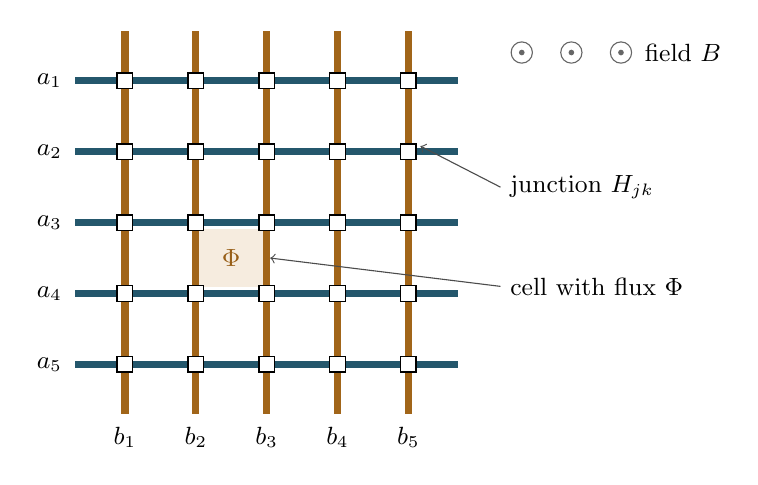
\begin{tikzpicture}[x=9mm,y=9mm,font=\small]
  \fill[glowgold!14] (1,1) rectangle (2,2);
  \node[glowgold!80!black] at (1.5,1.5) {$\Phi$};
  \foreach \k/\lab in {0/1,1/2,2/3,3/4,4/5}{
    \draw[glowgold!85!black,line width=2.6pt] (\k,-.7)--(\k,4.7);
    \node[below] at (\k,-.75) {$b_\lab$};
  }
  \foreach \j/\lab in {0/1,1/2,2/3,3/4,4/5}{
    \draw[white,line width=4.6pt] (-.7,4-\j)--(4.7,4-\j);
    \draw[glowblue,line width=2.6pt] (-.7,4-\j)--(4.7,4-\j);
    \node[left] at (-.75,4-\j) {$a_\lab$};
  }
  \foreach \j in {0,...,4}\foreach \k in {0,...,4}
    \filldraw[draw=black,fill=white,line width=.5pt] (\k-.11,\j-.11) rectangle (\k+.11,\j+.11);
  \draw[->,black!70] (5.3,2.5) node[right,text=black] {junction $H_{jk}$} -- (4.17,3.08);
  \draw[->,black!70] (5.3,1.1) node[right,text=black] {cell with flux $\Phi$} -- (2.05,1.5);
  \foreach \x/\y in {5.6/4.4,6.3/4.4,7.0/4.4}{
    \draw[black!60] (\x,\y) circle[radius=.15]; \fill[black!60] (\x,\y) circle[radius=.04];}
  \node[right] at (7.2,4.4) {field $B$};
\end{tikzpicture}
\caption{The crossed-wire array with $N=5$. The horizontal wires carry the phases $a_j$, the vertical wires the phases $b_k$, and a Josephson junction sits at each crossing. The magnetic field points towards the reader.}\label{fig:array}
\end{figure}

For a uniform field the phases can be computed in the Landau gauge. With wires at spacing $s$, and with $f=Bs^2/\Phi_0$ the flux through each cell, one finds $\theta_{jk}=2\pi fjk$, up to the choice of origin. Chandra, Ioffe and Sherrington write $f=\alpha/N$, calling $\alpha$ the flux per strip. At $\alpha=1$ the coupling matrix is the Fourier matrix:
\[
 H=F_N=\big(e^{2\pi ijk/N}\big)_{jk}
\]
The analytic glass calculation in \cite{cis} concerns weak fields, $1/N\ll\alpha\ll1$, where the coupling matrix is generally outside the Hadamard class. Chandra, Feigel'man and Ioffe \cite{cfi} found a dynamical instability in this regime, with diverging relaxation time and no coincident static transition. The Fourier point $\alpha=1$ gives a separate equilibrium problem.

\medskip
\noindent\textbf{Fluxes and gauge.}
Changing the reference phase of a wire multiplies the corresponding row or column of $H$ by a compensating phase. This simultaneous change of variables and couplings preserves the energy. Physical quantities depend on $H$ only through the products of its entries around closed loops, which are the fluxes. In a complete bipartite graph the cycles are generated by the $(N-1)^2$ cells between neighboring wires, and the cell fluxes determine everything else. Figure~\ref{fig:fluxes} gives three examples in their displayed wire order.

\begin{figure}[H]
\centering
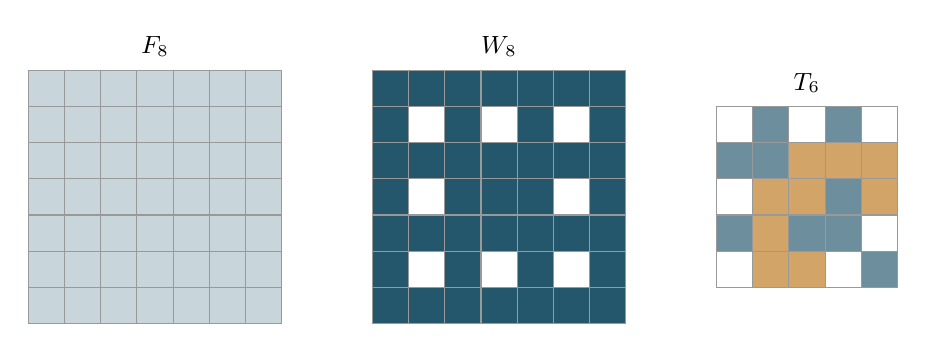
\begin{tikzpicture}[x=4.6mm,y=4.6mm,font=\small]
  \begin{scope}
    \foreach \j in {0,...,6}\foreach \k in {0,...,6}
      \fill[glowblue!25] (\k,-\j) rectangle ++(1,-1);
    \draw[step=1,black!40,thin] (0,-7) grid (7,0);
    \node[above] at (3.5,0.1) {$F_8$};
  \end{scope}
  \begin{scope}[shift={(9.5,0)}]
    \foreach \r [count=\j from 0] in {{1,1,1,1,1,1,1},{1,0,1,0,1,0,1},{1,1,1,1,1,1,1},{1,0,1,1,1,0,1},{1,1,1,1,1,1,1},{1,0,1,0,1,0,1},{1,1,1,1,1,1,1}}
      \foreach \v [count=\k from 0] in \r{
        \ifnum\v=1 \fill[glowblue] (\k,-\j) rectangle ++(1,-1);\fi}
    \draw[step=1,black!40,thin] (0,-7) grid (7,0);
    \node[above] at (3.5,0.1) {$W_8$};
  \end{scope}
  \begin{scope}[shift={(19,-1)}]
    \foreach \r [count=\j from 0] in {{0,1,0,1,0},{1,1,2,2,2},{0,2,2,1,2},{1,2,1,1,0},{0,2,2,0,1}}
      \foreach \v [count=\k from 0] in \r{
        \ifnum\v=1 \fill[glowblue!67] (\k,-\j) rectangle ++(1,-1);\fi
        \ifnum\v=2 \fill[glowgold!67] (\k,-\j) rectangle ++(1,-1);\fi}
    \draw[step=1,black!40,thin] (0,-5) grid (5,0);
    \node[above] at (2.5,0.1) {$T_6$};
  \end{scope}
\end{tikzpicture}
\caption{Cell fluxes of 3 Hadamard arrays, as computed by \texttt{fluxes.py}. The Fourier array $F_8$ has the uniform flux $1/8$. The Walsh array $W_8$ has fluxes 0 (white) and $1/2$ (dark), as every real Hadamard matrix. The Tao array $T_6$ has fluxes $0$, $1/3$ (blue) and $-1/3$ (gold).}\label{fig:fluxes}
\end{figure}

\begin{samepage}
\begin{prop}\label{prop:fluxes}
For $H\in M_N(\mathbb T)$ define the cell fluxes $\Phi_{jk}\in[0,1)$, in units of the flux quantum, by
\[
 e^{2\pi i\Phi_{jk}}=H_{jk}\bar H_{j+1,k}H_{j+1,k+1}\bar H_{j,k+1},\qquad 1\leq j,k\leq N-1
\]
Then the following hold:
\begin{enumerate}
\item 2 matrices have the same cell fluxes precisely when they differ by row and column phases, and every family of $(N-1)^2$ fluxes comes from a matrix.

\item For rows $a<b$ and columns $j<l$, the product $H_{aj}\bar H_{bj}H_{bl}\bar H_{al}$ equals $e^{2\pi i\Phi}$, where $\Phi$ is the total flux of the cells inside the rectangle with these corners.

\item $H$ is complex Hadamard precisely when every pair of rows $a<b$ satisfies
\[
 \sum_{j<l}\cos\big(2\pi\Phi(a,b;j,l)\big)=-N/2
\]
\end{enumerate}
\end{prop}
\end{samepage}
\begin{proof}
For the 1st assertion, the cell fluxes and the first row and column of $H$ determine the other entries, one cell at a time, and row and column phases can make the first row and column equal to 1. For the 2nd, the product of the cell holonomies over the rectangle telescopes, the interior edges cancelling in pairs. For the 3rd, write
\[
 \Big|\sum_jH_{aj}\bar H_{bj}\Big|^2=\sum_{jl}H_{aj}\bar H_{bj}H_{bl}\bar H_{al}
\]
where the $N$ terms with $j=l$ contribute 1 each and the other terms occur in conjugate pairs.
\end{proof}

Thus the equivalence class of a complex Hadamard matrix is the array up to gauge and renaming of the wires. Since every row wire interacts with every column wire, the order of the wires plays no role in the energy. The program \texttt{fluxes.py} checks these assertions numerically, and computes these three flux patterns. Physically, the condition $HH^*=N1_N$ says that the coupling matrix $H/\sqrt N$ between the 2 layers is unitary. The full interaction matrix of the $2N$ wires is $\left(\begin{smallmatrix}0&U\\U^*&0\end{smallmatrix}\right)$, with $U=H/\sqrt N$. Its square is the identity and its trace vanishes, so its eigenvalues are $+1$ and $-1$, each with multiplicity $N$. Such arrays are the complex analogs of the spin models with orthogonal interaction matrices of \cite{mp2,ppo}.

Figure~\ref{fig:cell} shows the effect of a gauge transformation on a single cell.

\begin{figure}[H]
\centering
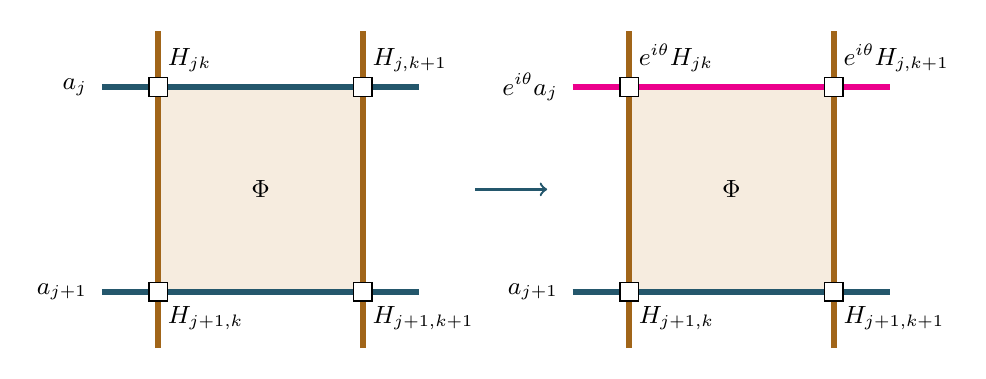
\begin{tikzpicture}[x=13mm,y=13mm,font=\small]
  \foreach \shift/\rot in {0/0,4.6/1}{
    \begin{scope}[shift={(\shift,0)}]
      \fill[glowgold!14] (0,0) rectangle (2,2);
      \node at (1,1) {$\Phi$};
      \draw[glowgold!85!black,line width=2.2pt] (0,-.55)--(0,2.55);
      \draw[glowgold!85!black,line width=2.2pt] (2,-.55)--(2,2.55);
      \ifnum\rot=1
        \draw[magenta,line width=2.2pt] (-.55,2)--(2.55,2);
      \else
        \draw[glowblue,line width=2.2pt] (-.55,2)--(2.55,2);
      \fi
      \draw[glowblue,line width=2.2pt] (-.55,0)--(2.55,0);
      \foreach \x/\y in {0/0,2/0,0/2,2/2}
        \filldraw[draw=black,fill=white,line width=.5pt] (\x-.09,\y-.09) rectangle (\x+.09,\y+.09);
      \ifnum\rot=1
        \node[above right] at (0,2.05) {$e^{i\theta}H_{jk}$};
        \node[above right] at (2,2.05) {$e^{i\theta}H_{j,k+1}$};
        \node[left] at (-.6,2) {$e^{i\theta}a_j$};
      \else
        \node[above right] at (0,2.05) {$H_{jk}$};
        \node[above right] at (2,2.05) {$H_{j,k+1}$};
        \node[left] at (-.6,2) {$a_j$};
      \fi
      \node[below right] at (0,-.05) {$H_{j+1,k}$};
      \node[below right] at (2,-.05) {$H_{j+1,k+1}$};
      \node[left] at (-.6,0) {$a_{j+1}$};
    \end{scope}}
  \draw[->,line width=.85pt,glowblue] (3.1,1)--(3.8,1);
\end{tikzpicture}
\caption{A gauge transformation rotates the phase of the wire $j$ by $\theta$, and multiplies the row $j$ of $H$ by $e^{i\theta}$. The energy does not change, and the 2 factors cancel in the flux $\Phi$ of every cell.}\label{fig:cell}
\end{figure}

\medskip
\noindent\textbf{A map of the paper.}
The array so far has junctions only between layers. In Section~\ref{sec:villain} we add Villain bonds of dimensionless stiffness $l$ within each layer. Figure~\ref{fig:map} treats the dimensionless junction strength $\beta$ and $l$ as independently variable coupling parameters. For fixed laboratory couplings both scale with inverse temperature. At $\beta=0$ the two layers are independent chains. The point $(0,0)$ gives the ordinary glow, and the expansion in $\beta$ along $l=0$ starts there. The lower right corner describes the junction ground states. On the left edge, taking $l\to\infty$ aligns each chain up to its own uniform phase.

\suppressfloats[t]
\begin{figure}[t]
\centering
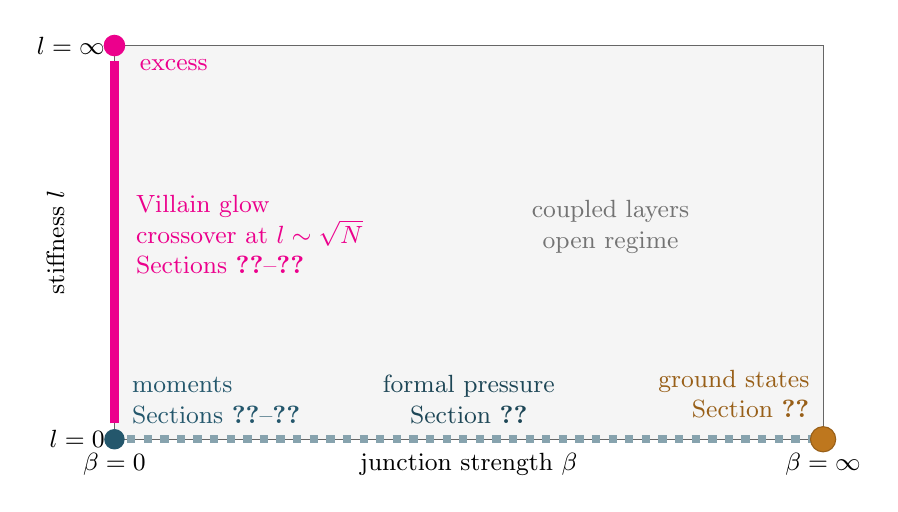
\begin{tikzpicture}[x=10mm,y=10mm,font=\small]
  \fill[black!4] (0,0) rectangle (9,5);
  \draw[black!60] (0,0) rectangle (9,5);
  \node[below] at (0,-.05) {$\beta=0$}; \node[below] at (9,-.05) {$\beta=\infty$};
  \node[below] at (4.5,-.05) {junction strength $\beta$};
  \node[left] at (0,0) {$l=0$}; \node[left] at (0,5) {$l=\infty$};
  \node[rotate=90] at (-.75,2.5) {stiffness $l$};
  \fill[glowblue] (0,0) circle[radius=.13];
  \node[above right,text=glowblue,align=left] at (.1,.08) {moments\\ Sections \ref{sec:moments}--\ref{sec:powers}};
  \draw[glowblue!55,line width=3pt,dashed] (.16,0)--(8.85,0);
  \node[above,text=glowblue!80!black,align=center] at (4.5,.08) {formal pressure\\ Section~\ref{sec:free}};
  \filldraw[draw=glowgold!80!black,fill=glowgold] (9,0) circle[radius=.16];
  \node[above left,text=glowgold!80!black,align=right] at (8.95,.15) {ground states\\ Section~\ref{sec:edge}};
  \draw[magenta,line width=3pt] (0,.2)--(0,4.8);
  \node[right,text=magenta,align=left] at (.15,2.6) {Villain glow\\ crossover at $l\sim\sqrt N$\\ Sections~\ref{sec:villain}--\ref{sec:general}};
  \filldraw[draw=magenta,fill=magenta] (0,5) circle[radius=.13];
  \node[right,text=magenta] at (.2,4.75) {excess};
  \node[text=black!55,align=center] at (6.3,2.7) {coupled layers\\ open regime};
\end{tikzpicture}
\caption{The parameters of the model. The bottom edge is the array of Section~\ref{sec:glow}, and the stiffness $l$ couples neighboring wires of each layer. The dots and solid line mark exact results. The dashed line indicates the fixed-temperature question suggested by the expansion at the origin.}\label{fig:map}
\end{figure}

\section{Glow moments and their polynomiality}\label{sec:moments}\label{sec:poly}

We now compute the high-temperature expansion of the array, that is, the moments of the glow of a general complex Hadamard matrix. We use the unnormalized variable $\Omega=NZ$ and retain the scalar-product convention of the introduction.

Let $H\in M_N(\mathbb T)$ be a complex Hadamard matrix. Following \cite{ba0,banica}, the glow of $H$ is the law of the variable
$$\Omega=\langle Hb,a\rangle=\sum_{ij}H_{ij}\bar a_ib_j$$
with $a,b\in\mathbb T^N$ independent and Haar distributed. This law is invariant under rotations, so it is determined by the moments $E(|\Omega|^{2p})$. It is convenient to encode them into the series
$$G(t)=\sum_{p\geq0}\frac{E(|\Omega|^{2p})}{p!^2}\,t^p=E\left[\exp\left(2\sqrt{t}\,Re(\Omega)\right)\right]$$
the second equality coming from $\int_\mathbb T\exp(Re(zs))ds=\sum_p|z|^{2p}/(4^pp!^2)$. Thus $G(\beta^2/(4N))$ is the partition function of the array at inverse temperature $\beta$, as in Proposition~\ref{prop:partition}.

Let $f(s)=\sum_{m\geq0}s^m/m!^2$, so that $E(|z_1s_1+\ldots+z_Ns_N|^{2p})=p!^2[t^p]\prod_if(t|z_i|^2)$ for $s\in\mathbb T^N$ Haar, and write $\log f(s)=\sum_k\kappa_ks^k$. We have $\kappa_1,\kappa_2,\kappa_3,\kappa_4=1,-\frac{1}{4},\frac{1}{9},-\frac{33}{576}$, and we set $w_k=k!\,\kappa_k$, so that $w_1,w_2,w_3,w_4=1,-\frac{1}{2},\frac{2}{3},-\frac{11}{8}$.

\begin{samepage}
\begin{thm}\label{thm:mom}
The glow moments of $H\in M_N(\mathbb T)$ are given by
$$E(|\Omega|^{2p})=p!\sum_{\pi\in P(p)}\Big(\prod_{\beta\in\pi}w_{|\beta|}\Big)N^{|\pi|}I(\pi)$$
where $I(\pi)=\frac{1}{N^{|\pi|}}\,\sum_{[i]=[j]}\prod_{\beta\in\pi}\big\langle\prod_{r\in\beta}C_{i_r},\prod_{r\in\beta}C_{j_r}\big\rangle$, with $C_1,\ldots,C_N\in\mathbb T^N$ being the columns of $H$, the products of vectors being taken componentwise, and with $[i]=[j]$ meaning that $i,j\in\{1,\ldots,N\}^p$ are equal as multisets.
\end{thm}
\end{samepage}

\begin{proof}
With $w=Hb$, we have $E_a(|\Omega|^{2p})=p!^2[t^p]\exp(\sum_k\kappa_kt^kS_k)$, where $S_k=\sum_x|w_x|^{2k}$. Expanding the exponential over the partitions of $\{1,\ldots,p\}$, the number of partitions with $\lambda_k$ blocks of size $k$ being $p!/\prod_k(k!^{\lambda_k}\lambda_k!)$, gives $E_a(|\Omega|^{2p})=p!\sum_\pi\prod_\beta w_{|\beta|}\prod_\beta S_{|\beta|}$. Finally, expanding $|w_x|^{2k}$ and integrating over $b$ gives $E_b\left(\prod_\beta S_{|\beta|}\right)=N^{|\pi|}I(\pi)$.
\end{proof}

This is the formula of \cite[Proposition 2.2]{banica}, with the coefficients $K(\pi)=\sum_\sigma\mu(\pi,\sigma)\binom{p}{\sigma}$ there identified as $K(\pi)=p!\prod_\beta w_{|\beta|}$, that is, as Steinhaus cumulants. Since $\Omega$ for $H$ and $H^t$ have the same law, the columns can be replaced by the rows. Figure~\ref{fig:bipartite} shows the interactions belonging to one row of the matrix.

\medskip
\suppressfloats[t]
\begin{figure}[t]
\centering
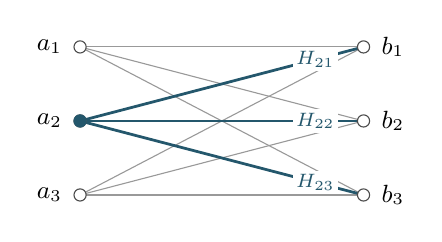
\begin{tikzpicture}[font=\small]
  \foreach \i in {1,2,3}{
    \coordinate (a\i) at (0,{2.05-.94*\i});
    \coordinate (b\i) at (3.6,{2.05-.94*\i});
  }
  \foreach \j in {1,3} \foreach \k in {1,2,3}
    \draw[black!40] (a\j)--(b\k);
  \foreach \k in {1,2,3} \draw[glowblue,line width=1pt] (a2)--(b\k);
  \foreach \i in {1,2,3}{
    \filldraw[draw=black!70,fill=white] (a\i) circle[radius=2.2pt];
    \filldraw[draw=black!70,fill=white] (b\i) circle[radius=2.2pt];
    \node[left=3pt] at (a\i) {$a_{\i}$};
    \node[right=3pt] at (b\i) {$b_{\i}$};
  }
  \fill[glowblue] (a2) circle[radius=2.4pt];
  \foreach \k/\name in {1/{H_{21}},2/{H_{22}},3/{H_{23}}}
    \path (a2)--(b\k) node[pos=.83,fill=white,inner sep=1.3pt,text=glowblue]
      {\scriptsize $\name$};
\end{tikzpicture}
\caption{The bipartite spin system for $N=3$. Each edge contributes
$H_{jk}\bar a_j b_k$ to $\Omega$. The 3 dark edges together contribute
$\bar a_2(Hb)_2$.}\label{fig:bipartite}
\end{figure}

\noindent\textbf{Polynomiality.}

For the Fourier matrix $F_G$ of a finite abelian group, the scalar products in $I(\pi)$ are $N$ or $0$, and so $I(\pi)$ counts the pairs $i,j\in G^p$ with $[i]=[j]$, and with $\sum_{r\in\beta}i_r=\sum_{r\in\beta}j_r$ for any $\beta\in\pi$ \cite[Proposition 3.1]{banica}.

\begin{samepage}
\begin{thm}\label{thm:poly}
Let $q$ be a prime, and $G=\mathbb Z_q^n$, with $N=q^n$. Then $E(|\Omega|^{2p})=P^{(q)}_p(N)$, where $P^{(q)}_p$ is a polynomial of degree $2p$, depending only on $q,p$. Moreover, $P^{(q)}_p=P^\infty_p$, a polynomial not depending on $q$, for $q$ larger than a constant $c_p$. In particular:
\begin{enumerate}
\item The glow moments of the Walsh matrices $W_N$, $N=2^n$, are polynomial in $N$.

\item The glow moments of the Fourier matrices $F_N$, with $N\geq c_p$ prime, are given by $P^\infty_p(N)$.
\end{enumerate}
\end{thm}
\end{samepage}

\begin{proof}
Given a pair $i,j\in G^p$ with $[i]=[j]$, let $v_1,\ldots,v_k$ be the distinct values of $i$ in order of first occurrence, and write $i_r=v_{f(r)}$ and $j_r=v_{g(r)}$. The conditions defining $I(\pi)$ read $\sum_cA_{\beta c}v_c=0$ for $\beta\in\pi$, with $A_{\beta c}=\#\{r\in\beta|f(r)=c\}-\#\{r\in\beta|g(r)=c\}$. Thus $I(\pi)$ is a sum, over the finitely many patterns $(f,g)$, which do not depend on $n$, of the numbers of solutions $v\in(\mathbb F_q^n)^k$ with distinct entries of the system $Av=0$. By M\"obius inversion on the partitions $\rho\in P(k)$, this number is
$$\sum_{\rho\in P(k)}\mu(0,\rho)\,N^{|\rho|-rk_q(A^\rho)}$$
where $A^\rho$ is obtained by adding the columns of $A$ over the blocks of $\rho$, because a linear system of rank $s$ in $m$ unknowns has $q^{n(m-s)}=N^{m-s}$ solutions in $(\mathbb F_q^n)^m$. Thus $I(\pi)$ and the moment are polynomials in $N$. To see the degree, put $z_i=(Hb)_i/N$, so $\sum_i|z_i|^2=1$. Coefficientwise, $f(t)\le e^t$ for nonnegative powers of $t$, hence the conditional phase-moment formula gives $E_a(|\Omega/N|^{2p})\le p!$. Jensen's inequality and $E(|\Omega/N|^2)=1$ give the lower bound 1 after averaging. The polynomial therefore has degree exactly $2p$. Finally, the row of $A^\rho$ indexed by $\beta$ has sum of absolute values at most $2|\beta|$. By Hadamard's determinant inequality every minor has absolute value at most $\prod_{\beta\ \mathrm{selected}}2|\beta|\le 2^p$, since $2d\le2^d$ for $d\ge1$. Thus for every prime $q>2^p$ the rank equals the rational rank. This sufficient bound applies to all the patterns at once.
\end{proof}

This settles the conjecture in \cite[section 4]{banica}, that the glow of $W_N$ is polynomial in $N$. Note that the polynomials are valid for all $n\geq0$, the factors which vanish at small $N$ taking care of themselves. The same argument works for the real glow of the real Walsh matrices, with $a,b\in\{\pm1\}^N$.

\medskip

\noindent\textbf{Computation.} All the programs used in this paper are in the code folder, together with their outputs, as files of type \texttt{.out}, \texttt{.log}, \texttt{.csv} and \texttt{.json}, the shell script \texttt{runall.sh} rerunning the faster ones. We computed the polynomials $P^{(q)}_p$ exactly, by implementing the above proof, in the programs \texttt{walshglow.py}, for $q=2$, and \texttt{fqglow.py}, for $q$ prime, for $q=2,3,5,7,11,13$ and $p\leq7$, and through $p=8$ for Walsh and the generic case. For example $q=1000003>2^8$ computes the generic ranks throughout this range. For the Walsh matrices, $P_p=P^{(2)}_p$, we obtain:
\begin{eqnarray*}
P_1&=&N^2\\
P_2&=&2N^4-2N^3+N^2\\
P_3&=&6N^6-18N^5+33N^4-36N^3+16N^2\\
P_4&=&24N^8-144N^7+528N^6-1368N^5+2452N^4-2580N^3+1089N^2\\
P_5&=&120N^{10}-1200N^9+7200N^8-31800N^7+108020N^6-276500N^5\\
&&+492025N^4-505800N^3+207936N^2\\
P_6&=&720N^{12}-10800N^{11}+95400N^{10}-626400N^9+3279120N^8-13917600N^7\\
&&+47176350N^6-121830750N^5+216851921N^4-220509560N^3+89491600N^2
\end{eqnarray*}
and $P_7,P_8$ are in the file \texttt{walsh.out}. As checks, these polynomials give 1 at $N=1$, as they should, and their values at $N=2,4,8$ agree numerically with direct torus quadrature. A grid of $p+1$ equally spaced phases per coordinate is an exact quadrature rule for this moment, by character orthogonality. The comparisons are made by the programs \texttt{check.py} and \texttt{check2.py}, through $p=8$ at $N=2,4$, and $p\leq6$ at $N=8$. Similarly, the polynomials $P^{(3)}_p$ agree with the quadrature for $F_3$ and $\mathbb Z_3^2$, and $P^\infty_p$ agrees with it for $F_5$ and $F_7$. We also find that $[N^2]P_p=(p!^2\kappa_p)^2$, the numbers $p!^2|\kappa_p|$ being $1,1,4,33,456,9460,274800,10643745$, and that this lowest coefficient is the same for all $q$.


The block construction in \cite{dita} gives families of Hadamard matrices
with free phase parameters. These suggest the following extension of the polynomial calculation.

\begin{samepage}
\begin{question}\label{que:families}
Compute glow polynomials for other families of complex Hadamard matrices, including Di\c t\u a deformations of Fourier matrices. How do their coefficients, and the associated free-energy terms, compare with the quantum invariants and the defect?
\end{question}
\end{samepage}

\section{Walsh and generic Fourier moments}\label{sec:walsh}

Walsh arrays have fluxes 0 and $1/2$ only. For $\mathbb Z_q^n$ in sufficiently large characteristic, the moment at any prescribed order has the generic polynomial value. We now compare the 2 families.

The polynomials $P^\infty_p$ agree with the Walsh ones for $p\leq3$, and then:
\begin{eqnarray*}
P_4-P^\infty_4&=&18N^3(N-1)\\
P_5-P^\infty_5&=&N^3(N-1)(450N^2-3600N+9600)\\
P_6-P^\infty_6&=&N^3(N-1)(8100N^4-137700N^3+1065150N^2-4441500N+7663500)
\end{eqnarray*}
For $q=3$ the first deviation is at $p=6$, with $P^{(3)}_6-P^\infty_6=N^3(N-1)(21600N+51200)$, and for $q=5,7,11,13$ there is no deviation at $p\leq7$, these differences being factored by the program \texttt{diff.py}. Normalizing as in \cite{banica}, we have
$$\frac{1}{p!}\,E\left[\left(\frac{|\Omega|}{N}\right)^{2p}\right]=1-\frac{K_1}{N}+\frac{K_2}{N^2}-\frac{K_3}{N^3}+\frac{K_4}{N^4}-\ldots$$
and in terms of the basis $\binom{p}{j}$ our data gives:

\medskip

\begin{center}
\begin{tabular}{lllllll}
\toprule
& $\binom{p}{3}$ & $\binom{p}{4}$ & $\binom{p}{5}$ & $\binom{p}{6}$ & $\binom{p}{7}$ & $\binom{p}{8}$\\
\midrule
$K_3$, all $q$ & 6 & 33 & 40 & 15 & & \\
$K_4$, generic & $\frac{8}{3}$ & $\frac{363}{4}$ & 416 & $\frac{1265}{2}$ & 420 & 105\\
$K_4$, Walsh & $\frac{8}{3}$ & $\frac{183}{2}$ & 416 & $\frac{1265}{2}$ & 420 & 105\\
\bottomrule
\end{tabular}
\end{center}

\medskip

\noindent The values of $K_1,K_2,K_3$ are those of \cite[Theorem 3.6]{banica}. The $K_4$ rows are interpolations from $3\leq p\leq8$, done by the program \texttt{look.py}, with the top coefficient $105=7!!$ as expected from the Gaussian limit, and are to be confirmed at $p=9$. Their difference is however exact:

\begin{samepage}
\begin{thm}\label{thm:k4}
We have $K_4^{Walsh}-K_4^\infty=\frac{3}{4}\,\binom{p}{4}$, at all $p$.
\end{thm}
\end{samepage}

\begin{proof}
Write $B_q(z)=\sum_{k\ge0}P_k^{(q)}(N)z^k/((k!)^2N^{2k})$, with $P_0^{(q)}=1$, and use the same notation for the generic polynomials. By Theorem~\ref{thm:free-leading}, the coefficient of $z^k$ in $\log B_q$ is $C_k^{(q)}(N)/N^{2k}$, where the term of degree $k+1$ in $C_k^{(q)}$ is independent of $q$. This also holds for the generic coefficient by taking $q$ sufficiently large at each fixed order. The first three coefficients agree exactly by Theorem~\ref{thm:s2}. At $k=4$ that theorem gives
\[
 C_4^{(2)}(N)-C_4^\infty(N)
 =\frac{18N^3(N-1)}{(4!)^2}=\frac{N^4-N^3}{32}
\]
For $k\ge5$ the normalized difference is $O_k(N^{-k})$. Hence, coefficientwise in $z$,
\[
 \log B_2-\log B_\infty=\frac{z^4}{32N^4}+O(N^{-5}),
 \qquad B_\infty=e^z+O(N^{-1})
\]
The second identity follows from $C_1=N^2$ and the same degree bound. Exponentiating and extracting $p![z^p]$ gives the difference in $K_4$ as $p![z^p](e^zz^4/32)=\tfrac34\binom p4$, including $p<4$.
\end{proof}

Figure~\ref{fig:blocks} shows a pair of blocks that detects the characteristic at the 8th moment.

\begin{figure}[htb!]
\centering
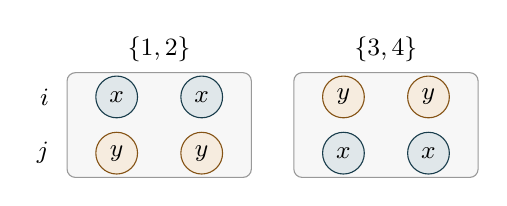
\begin{tikzpicture}[x=9mm,y=7mm,font=\small]
  \foreach \left/\right/\middle/\positions in
      {0/2.6/1.3/{1,2},3.2/5.8/4.5/{3,4}}{
    \filldraw[fill=black!3,draw=black!40,rounded corners=3pt]
      (\left,-.44) rectangle (\right,1.46);
    \node[above] at (\middle,1.48) {$\{\positions\}$};
  }
  \node[left] at (-.12,1.02) {$i$};
  \node[left] at (-.12,0) {$j$};
  \foreach \u/\v/\letter/\shade in
      {.7/1.02/x/glowblue,1.9/1.02/x/glowblue,3.9/1.02/y/glowgold,5.1/1.02/y/glowgold,
       .7/0/y/glowgold,1.9/0/y/glowgold,3.9/0/x/glowblue,5.1/0/x/glowblue}
    \node[draw=\shade!70!black,fill=\shade!14,circle,minimum size=5.3mm,inner sep=0pt]
      at (\u,\v) {$\letter$};
\end{tikzpicture}
\caption{In each block the sum of the top labels must equal the sum of
the bottom labels. Both conditions reduce to $2x=2y$. In a Walsh group
every choice of distinct $x,y$ survives.}\label{fig:blocks}
\end{figure}

The Walsh correction already appears at $p=4$, and the characteristic-3 correction at $p=6$. The computations suggest that characteristic $q$ first changes the generic polynomial at $p=2q$. The natural candidate for the universal measure $\mu_N$ asked for in \cite[section 4]{banica} is the one with moments $P^\infty_p(N)$, whose polynomial values are defined for all $N$. For each fixed $p$, these values agree with the glow of $F_N$ for sufficiently large prime $N$. At a fixed $N$, however, positivity of the full moment sequence would be an additional requirement.

In fact, this proposed measure fails to exist already at $N=2$. Direct evaluation gives
\[
 P^\infty_1(2)=4,\quad P^\infty_2(2)=20,\quad
 P^\infty_3(2)=112,\quad P^\infty_4(2)=532
\]
so that the Hankel matrix of the candidate moments of $|\Omega|^2$ satisfies
\[
 \det\begin{pmatrix}1&4&20\\4&20&112\\20&112&532\end{pmatrix}=-496<0
\]
whereas a moment matrix of a probability measure is positive semidefinite. Moreover, $P^\infty_5(2)=-29296$. These values are computed by the program \texttt{hankel.py}, which also checks that the Walsh values $P_p(2)$, which are the moments of $F_2$, give positive Hankel minors. Thus the generic polynomials describe fixed-order formulas valid in sufficiently large characteristic; their evaluations at an arbitrary fixed $N$ need not define a probability law.


The computed rows of $K_4$ also suggest continuing the exact enumeration.

\begin{samepage}
\begin{question}\label{que:enumerate}
Compute $P_p$ at $p=9,10$, test the interpolated $K_4$ formulas, and determine $K_5$. Can the all-order coefficients be obtained directly from the partition expansion?
\end{question}
\end{samepage}

\section{Hadamard powers and plaquette fluxes}\label{sec:powers}

For $H\in M_N(\mathbb T)$ and $k\in\mathbb N$, consider the Hadamard power $H^{\circ k}=(H_{ij}^k)$, and the quantity
$$S_k(H)=\big\|H^{\circ k}(H^{\circ k})^*-N1_N\big\|^2=\sum_{x\neq y}\big|\langle C_x^k,C_y^k\rangle\big|^2$$
with the Hilbert--Schmidt norm, which vanishes precisely when $H^{\circ k}$ is Hadamard. Since $\|KK^*\|=\|K^*K\|$, we can use either rows or columns, and $S_k$ is invariant under the equivalence of complex Hadamard matrices, and under transposition. For the Fourier matrices we have $S_k(F_G)=N^3(|G[k]|-1)$, where $G[k]=\{x\in G|kx=0\}$, so the $S_k$ detect the torsion of $G$. The generic polynomials $P^\infty_p$ are obtained from Fourier matrices in sufficiently large prime characteristic. The quantities $S_k$ record some of the deviations from these polynomials.

\medskip
\noindent\textbf{Flux harmonics.}
A junction with a $k$th harmonic in its current--phase relation has a term proportional to $\sin(k(\varphi_a-\psi_j-\theta_{aj}))$. Its magnetic phase is $H_{aj}^k$, so the corresponding rectangle sees $k$ times the original flux. The same harmonics arise here from products of the fundamental junction terms in the moment expansion. Thus the moments of the sinusoidal model already detect the failure of $H^{\circ k}$ to be Hadamard. In terms of fluxes, the rectangle holonomies of Proposition~\ref{prop:fluxes} give the following picture, illustrated in Figure~\ref{fig:rectangle}.

\begin{samepage}
\begin{prop}\label{prop:harmonics}
For $H\in M_N(\mathbb T)$, write $\Phi(a,b;j,l)$ for the flux through the rectangle with horizontal sides on the row wires $a,b$ and vertical sides on the column wires $j,l$, oriented as in Proposition~\ref{prop:fluxes}. Then
\[
 S_k(H)=\sum_{a\neq b}\sum_{jl}\cos\big(2\pi k\,\Phi(a,b;j,l)\big)
\]
where the sum includes $\Phi(a,b;j,j)=0$. Equivalently, counting only distinct unoriented rectangles gives $N^2(N-1)+4\sum_{a<b,\ j<l}\cos(2\pi k\Phi(a,b;j,l))$.
\end{prop}
\end{samepage}
\begin{proof}
Expanding the squared modulus, we have
\[
 \Big|\sum_jH_{aj}^k\bar H_{bj}^k\Big|^2=\sum_{jl}\big(H_{aj}\bar H_{bj}H_{bl}\bar H_{al}\big)^k=\sum_{jl}e^{2\pi ik\Phi(a,b;j,l)}
\]
and the sum is real, since exchanging $j$ and $l$ conjugates each term. Summing over $a\neq b$ gives $S_k(H)$, and the case $k=1$ is Proposition~\ref{prop:fluxes}.
\end{proof}

The program \texttt{fluxes.py} also checks this formula for $k=2,3$. In the language of lattice gauge theory, the products $H_{aj}\bar H_{bj}H_{bl}\bar H_{al}$ are Wilson loops, the gauge invariant observables introduced by Wilson to study the confinement of quarks \cite{wil}, and $S_k$ is the sum of the Wilson loops of charge $k$ over the rectangles. A real Hadamard matrix has all its fluxes equal to 0 or $1/2$, so that all its Wilson loops of charge 2 are equal to 1, and $S_2$ is maximal. This is the content of Corollary~\ref{cor:extreme} below. The cubic invariants $R$ and $T$ are built in the same way on 3 row wires and 3 column wires.

\begin{figure}[htb!]
\centering
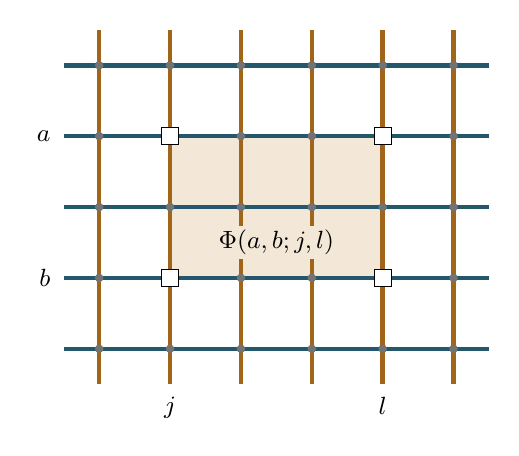
\begin{tikzpicture}[x=9mm,y=9mm,font=\small]
  \fill[glowgold!18] (1,1) rectangle (4,3);
  \foreach \k in {0,...,5}
    \draw[glowgold!85!black,line width=1.6pt] (\k,-.5)--(\k,4.5);
  \foreach \j in {0,...,4}
    \draw[glowblue,line width=1.6pt] (-.5,\j)--(5.5,\j);
  \node[fill=glowgold!18,inner sep=1.5pt] at (2.5,1.5) {$\Phi(a,b;j,l)$};
  \foreach \j in {0,...,4}\foreach \k in {0,...,5}
    \fill[black!55] (\k,\j) circle[radius=.06];
  \foreach \x/\y in {1/1,4/1,1/3,4/3}
    \filldraw[draw=black,fill=white] (\x-.12,\y-.12) rectangle (\x+.12,\y+.12);
  \node[left] at (-.55,3) {$a$}; \node[left] at (-.55,1) {$b$};
  \node[below] at (1,-.55) {$j$}; \node[below] at (4,-.55) {$l$};
\end{tikzpicture}
\caption{A rectangle in the array, with corners at the junctions $aj,al,bj,bl$. The product of the junction phases around it is $e^{2\pi i\Phi}$, where $\Phi$ is the flux through the shaded region.}\label{fig:rectangle}
\end{figure}

\medskip
\noindent\textbf{The 8th and 10th moments.}
The first 2 non-universal moments can be evaluated together. The calculation uses the joint distribution of 2 distinct row sums. For the following lemma all the phases $b_j$ are independent and uniform.

\begin{samepage}
\begin{lem}\label{lem:rowpairs}
Let $X=\sum_jb_j$ and $Y=\sum_ju_jb_j$, where $u_j\in\mathbb T$ and $\sum_ju_j=0$. With $Q=\sum_ju_j^2$, we have
\[
 E(|X|^4|Y|^4)
 =4N^4-20N^3+41N^2-33N+|Q|^2
\]
and
\[
 E(|X|^6|Y|^4)
 =12N^5-96N^4+341N^3-613N^2+456N+(9N-24)|Q|^2
\]
for every such pair of orthogonal unimodular rows.
\end{lem}
\end{samepage}
\begin{proof}
Use 4 formal variables $z,v,t,s$, and set $A=zv$, $B=ts$, $C=tv$, $D=zs$, so that $CD=AB$. Independence and phase integration give
\[
 E\big[\exp(zX+v\bar X+tY+s\bar Y)\big]
   =\prod_{j=1}^N f\big[(z+tu_j)(v+s\bar u_j)\big]
\]
with $f$ from Section~\ref{sec:moments}. The moment with exponents $2a,2b$ is $(a!b!)^2$ times the coefficient of $z^av^at^bs^b$ in this series.

Write $L$ for its logarithm. The terms independent of the powers of $u_j$ form
\[
 L_0=N\sum_{m\ge1}\kappa_m
            \sum_{r=0}^m\binom mr^2 A^rB^{m-r}
\]
by expanding the 2 binomials before summing over $j$. Terms involving $\sum_ju_j$ or its conjugate vanish. Since we need $b=2$, terms involving powers $u_j^h$ with $|h|\ge3$ already have too high a degree in $t$ or $s$. The remaining nonconstant terms can contribute to our balanced coefficients only in pairs, one containing $Q$ and the other $\bar Q$. Up to total bidegree $(5,5)$ the terms needed for this pairing are
\[
 \big(\kappa_2+3\kappa_3(A+B)\big)(QC^2+\bar QD^2)
\]
where bidegree counts the variables $(z,t)$ and $(v,s)$ separately. A term of degree at least 4 containing $Q$ needs a conjugate term of degree at least 2, hence contributes only from total bidegree $(6,6)$ onward.

In $\exp L$, the coefficient of $|Q|^2A^2B^2$ is therefore $\kappa_2^2=1/16$. The coefficient of $|Q|^2A^3B^2$ is
\[
 N\kappa_2^2+6\kappa_2\kappa_3=\frac{N}{16}-\frac16
\]
the first term coming from the factor $NA$ in $\exp L_0$. Multiplication by $16$ and $144$ gives the stated coefficients $1$ and $9N-24$.

For the constant parts, direct expansion of $\exp L_0$ gives
\[
 [A^2B^2]\exp L_0=\frac{4N^4-20N^3+41N^2-33N}{16}
\]
and
\[
 [A^3B^2]\exp L_0
   =\frac{12N^5-96N^4+341N^3-613N^2+456N}{144}
\]
using $\kappa_1=1$, $\kappa_2=-1/4$, $\kappa_3=1/9$, $\kappa_4=-11/192$, $\kappa_5=19/600$. This proves both identities.
\end{proof}

Summing over pairs of rows turns $|Q|^2$ into $S_2(H)$. This gives the following exact extension of the 8th-moment formula.

\begin{samepage}
\begin{thm}\label{thm:s2}
For any complex Hadamard matrix $H\in M_N(\mathbb T)$, we have
\[
 E(|\Omega|^{2p})=P^\infty_p(N)\qquad (p\le3)
\]
as well as
\[
 E(|\Omega|^8)=P^\infty_4(N)+18S_2(H)
\]
and
\[
 E(|\Omega|^{10})
   =P^\infty_5(N)+(450N^2-3600N+9600)S_2(H)
\]
so the same Hadamard-square invariant controls the first 2 non-universal moments.
\end{thm}
\end{samepage}
\begin{proof}
Put $w=Hb$ and $T_r=\sum_x|w_x|^{2r}$. Orthogonality gives $T_1=N^2$ deterministically. The expectation of each $T_r$ is universal, since every row sum has the law of a sum of $N$ uniform phases. More precisely, with
\[
 m_r=(r!)^2[t^r]f(t)^N
\]
we have $E(T_r)=Nm_r$. The first 5 values are
\[
 m_1=N,\qquad m_2=2N^2-N,\qquad m_3=6N^3-9N^2+4N
\]
and
\[
 m_4=24N^4-72N^3+82N^2-33N
\]
and
\[
 m_5=120N^5-600N^4+1250N^3-1225N^2+456N
\]
by the same phase integration.

For distinct rows $x,y$, absorb the phases of the first row into $b$. The ratio of the 2 rows gives the $u_j$ of Lemma~\ref{lem:rowpairs}. Their sum is 0 by orthogonality, and the sum of the corresponding $|Q|^2$ over ordered distinct rows is $S_2(H)$. The equal-row contributions are $Nm_4$ and $Nm_5$. Summing the lemma therefore gives
\[
 E(T_2^2)=4N^6-11N^4+8N^3+S_2(H)
\]
and
\[
 E(T_3T_2)
 =12N^7+12N^6-163N^5+296N^4-156N^3+(9N-24)S_2(H)
\]
after collecting powers of $N$.

Conditional integration over $a$ now reads
\[
 E_a(|\Omega|^{2p})
  =(p!)^2[t^p]\exp\left(N^2t+\sum_{r\ge2}\kappa_rT_rt^r\right)
\]
so through degree 3 only the universal single expectations occur. In degree 4 the only additional term is $\kappa_2^2E(T_2^2)/2$, giving coefficient $4!^2\kappa_2^2/2=18$ on $S_2(H)$. In degree 5 the 2 additional terms are
\[
 \frac{N^2\kappa_2^2}{2}\,E(T_2^2)
       +\kappa_2\kappa_3E(T_2T_3)
\]
and their coefficient on $S_2(H)$, after multiplication by $5!^2$, is
\[
 5!^2\left(\frac{N^2}{32}-\frac{9N-24}{36}\right)
      =450N^2-3600N+9600
\]
as asserted. All remaining terms are universal polynomials in $N$. For arbitrarily large prime $N$, the matrix $F_N$ has $S_2(F_N)=0$. Polynomiality then identifies these remaining polynomials with $P^\infty_4$ and $P^\infty_5$.
\end{proof}

For the Walsh matrices $S_2=N^3(N-1)$, recovering the differences at $p=4,5$ in Section~\ref{sec:walsh}. The data set contains 33 matrix examples of orders 6 to 12, including Fourier matrices, Di\c t\u a deformations and non-Di\c t\u a examples. The computations reach the 8th moment in 32 cases and the 10th moment in 28, which suggested the two identities. The matrices are defined in \texttt{matrices.py} and \texttt{cases.py}, their moments are computed by the program \texttt{basisglow.py}, and compared with $S_2,S_3$ by \texttt{s2check.py} and \texttt{s2s3fit.py}. Theorem~\ref{thm:s2} proves it for every complex Hadamard matrix.

The positive coefficients in these 2 formulas also identify their extremizers.

\begin{samepage}
\begin{cor}\label{cor:extreme}
For $p=4,5$, put $a_4(N)=18$ and $a_5(N)=450N^2-3600N+9600$. Then
\[
 P^\infty_p(N)\le E(|\Omega|^{2p})
       \le P^\infty_p(N)+a_p(N)N^3(N-1)
\]
for every complex Hadamard matrix of order $N$. Equality on the left holds exactly when $H^{\circ2}$ is Hadamard. Equality on the right holds exactly when $H$ is equivalent to a real Hadamard matrix.
\end{cor}
\end{samepage}
\begin{proof}
Each scalar product between 2 squared rows has modulus at most $N$. Hence $0\le S_2(H)\le N^3(N-1)$. Also
\[
 a_5(N)=450(N-4)^2+2400>0
\]
so Theorem~\ref{thm:s2} gives the bounds and the lower equality case. Equality in the upper bound means that every 2 squared rows are proportional. Thus $H^{\circ2}$ has rank 1. Write $H_{ij}^2=r_ic_j$ with $r_i,c_j\in\mathbb T$, choose square roots, and remove them by row and column phases. The resulting Hadamard matrix has entries in $\{1,-1\}$. Conversely every matrix equivalent to a real Hadamard matrix has a rank-1 square and attains this bound.
\end{proof}

The invariant $S_2$ can vary even along an affine 1-parameter family. For instance,
\[
 H(a)=
 \begin{pmatrix}
 1&1&1&1\\
 1&a&-1&-a\\
 1&-1&1&-1\\
 1&-a&-1&a
 \end{pmatrix},\qquad a=e^{it}
\]
is Hadamard for all $a\in\mathbb T$, and
\[
 S_2(H(a))=64+32|1+a^2|^2=64+128\cos^2t
\]
by taking scalar products of its squared rows. At $a=1$ it is Walsh, while at $a=i$ it is $F_4$. Thus the constancy observed along some of the families below is a property of those particular families.
Figure~\ref{fig:grams} shows which pairs of squared rows contribute to
the change from the Walsh matrix to $F_4$.

\begin{figure}[htb!]
\centering
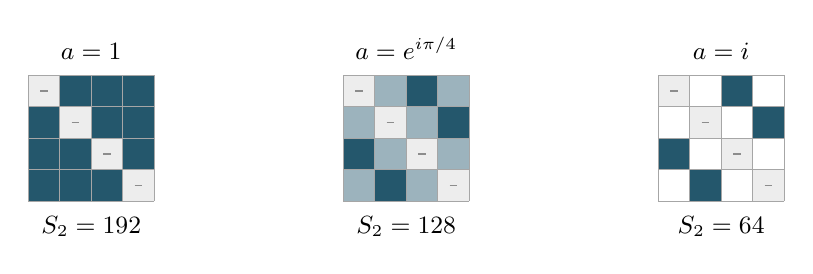
\begin{tikzpicture}[x=4mm,y=4mm,font=\small]
  \foreach \shift/\angle/\value/\labela in {0/0/192/1,10/45/128/{e^{i\pi/4}},20/90/64/i}{
    \begin{scope}[shift={(\shift,0)}]
      \foreach \r in {0,...,3}{
        \foreach \c in {0,...,3}{
          \ifnum\r=\c
            \fill[black!7] (\c,-\r) rectangle ++(1,-1);
            \draw[black!45] (\c+.38,-\r-.5)--(\c+.62,-\r-.5);
          \else
            \pgfmathtruncatemacro{\level}{mod(\r-\c,2)==0 ? 16 : round(16*cos(\angle)^2)}
            \ifnum\level=16 \fill[glowblue] (\c,-\r) rectangle ++(1,-1);\fi
            \ifnum\level=8 \fill[glowblue!45] (\c,-\r) rectangle ++(1,-1);\fi
          \fi
        }
      }
      \draw[step=1,thin,black!35] (0,-4) grid (4,0);
      \node[above=2pt] at (2,0) {$a=\labela$};
      \node[below=2pt] at (2,-4) {$S_2=\value$};
    \end{scope}
  }
\end{tikzpicture}
\caption{Squared row correlations $|\langle h_r^{\circ2},h_s^{\circ2}\rangle|^2$
for $H(a)$. Dark, medium and white off-diagonal cells have values 16, 8 and 0.
Their sum is $S_2$. The diagonal is omitted.}\label{fig:grams}
\end{figure}



\medskip
\noindent\textbf{The 12th moment.}
At the next order there are 2 cubic contractions to consider. Write $h_a$ for row $a$ of $H$, and put
\[
 B=H^{\circ2}(H^{\circ2})^*-N1_N,\qquad
 Q_{abc}=\sum_jH_{aj}^2\bar H_{bj}\bar H_{cj}
\]
so that $B_{aa}=0$ and $S_2(H)=Tr(B^2)$. We use the real invariants
\[
 R(H)=Tr(B^3),\qquad
 T(H)=Re\sum_{\substack{abc\\\text{pairwise distinct}}}
                         Q_{abc}Q_{bca}Q_{cab}
\]
where the sum is over ordered triples. The first is determined by the singular values of $H^{\circ2}$. The second combines 3 different rows before summing over the columns.

Both quantities are invariant under Hadamard equivalence. For $R$ this follows from conjugation of the Gram matrix by row phases. For $T$, the row phases cancel in each product and the column phases cancel in each $Q_{abc}$. Both invariants are also unchanged by transposition. This is immediate from singular values for $R$. For $T$, orthogonality gives $Q_{aab}=0$ if $a\ne b$, and $Q_{aaa}=N$, so
\[
 T(H)+N^4=Re\sum_{abc}\sum_{ijk}
 H_{ai}^2H_{bj}^2H_{ck}^2
 \bar H_{bi}\bar H_{ci}\bar H_{aj}\bar H_{cj}\bar H_{ak}\bar H_{bk}
\]
which is unchanged by exchanging the row triple with the column triple.

The mixed row sums from the proof of Theorem~\ref{thm:s2} have the following extensions. We retain $T_r=\sum_a|(Hb)_a|^{2r}$, with independent uniform phases $b_j$.

\begin{samepage}
\begin{lem}\label{lem:sixmixed}
There are polynomials $U_{42},U_{33},U_{222}$, independent of $H$, such that
\[
 E(T_4T_2)=U_{42}(N)+(72N^2-420N+652)S_2(H)
\]
and
\[
 E(T_3^2)=U_{33}(N)+(81N^2-513N+882)S_2(H)+16S_3(H)
\]
and
\[
 E(T_2^3)=U_{222}(N)+(6N^3+57N^2-240N)S_2(H)-2R(H)-16T(H)
\]
for every complex Hadamard matrix of order $N$.
\end{lem}
\end{samepage}
\begin{proof}
We give a finite coefficient calculation for the constants and the new terms. For $d$ distinct rows, introduce variables $x_1,\ldots,x_d,y_1,\ldots,y_d$, and put $X_i=(Hb)_{a_i}$. With multi-indices $r,s$, the logarithm of their joint generating function is
\[
 \log E\left[\exp\left(\sum_i x_iX_i+y_i\bar X_i\right)\right]
   =\sum_{|r|=|s|=m\ge1}
       \kappa_m\binom mr\binom ms x^ry^s
       \sum_j\prod_iH_{a_i j}^{r_i-s_i}
\]
where $\binom mr=m!/\prod_i r_i!$. The exponents $r_i-s_i$ may be negative because the entries have modulus 1. Each mixed moment is the coefficient of $x^uy^u$ multiplied by $\prod_i(u_i!)^2$.

For 2 rows the charge $r-s=(1,-1)$ vanishes by orthogonality. Through bidegree $(6,6)$, only a charge and its negative can contribute nonconstant terms. Charges $(2,-2)$ give $|\sum_jH_{aj}^2\bar H_{bj}^2|^2$, and $(3,-3)$ give the analogous cube. The resulting coefficients are
\[
\begin{array}{c|cc}
 u & \text{square of charge }(2,-2)&\text{square of charge }(3,-3)\\
 \hline
 (4,2)&72N^2-420N+652&0\\
 (3,3)&81N^2-513N+882&16
\end{array}
\]
with universal constant terms. Summing the distinct-row terms gives $S_2,S_3$. Equal-row contributions depend only on $N$.

For clarity, the entries in this table and the next can be extracted without any infinite expansion. For a fixed exponent bound $u$ define the finite polynomials
\[
 L_e=\sum_{\substack{0\le r,s\le u\\r-s=e\\|r|=|s|\ge1}}
           \kappa_{|r|}\binom{|r|}{r}\binom{|s|}{s}x^ry^s
\]
so that the charge-0 part of the logarithm is $NL_0$. The coefficient of the squared modulus of the charge $e$ is
\[
 \left(\prod_i(u_i!)^2\right)
 [x^uy^u]\exp(NL_0)L_eL_{-e}
\]
and all terms above the bounds $u$ can be discarded. For these tables only $\kappa_1,\ldots,\kappa_4$ are needed. This expression gives the displayed polynomials using $1,-1/4,1/9,-11/192$.

Now take 3 distinct rows and $u=(2,2,2)$. The nonzero charges, apart from 0 itself, are permutations of $(2,-2,0)$ and $(2,-1,-1)$ and their negatives. Charges of type $(1,-1,0)$ vanish. Balanced products are pairs of opposite charges, or triangles of 3 charges of the same type. Write
\[
 P_{ab}=\sum_jH_{aj}^2\bar H_{bj}^2,\quad
 Q_a=Q_{abc},\quad Q_b=Q_{bca},\quad Q_c=Q_{cab}
\]
for this fixed triple. The nonconstant terms in $E(|X_aX_bX_c|^4)$ are
\[
 (2N^2-33N+130)(|P_{ab}|^2+|P_{bc}|^2+|P_{ca}|^2)
\]
plus
\[
 (16N^2-144N+392)(|Q_a|^2+|Q_b|^2+|Q_c|^2)
       -2Re(P_{ab}P_{bc}P_{ca})-16Re(Q_aQ_bQ_c)
\]
by the same finite extraction. For the triangles, the calculation is particularly short. A pair charge first appears with coefficient $\kappa_2$, so the 2 orientations contribute $2(2!)^6\kappa_2^3=-2$. A split charge first appears with coefficient $2\kappa_2$, giving $2(2!)^6(2\kappa_2)^3=-16$.

It remains to sum over row triples. Orthogonality twice gives
\[
 \sum_{abc}|Q_{abc}|^2
   =\sum_{jk}\left(\sum_aH_{aj}^2\bar H_{ak}^2\right)
                  \left(\sum_b\bar H_{bj}H_{bk}\right)^2=N^4
\]
and hence the sum over pairwise distinct triples is $N^4-N^3-S_2(H)$. The sum of the 3 pair squares over distinct triples is $3(N-2)S_2(H)$, and the sum of the 3 split squares is $3(N^4-N^3-S_2(H))$. The 2 triangle sums give $R(H)$ and $T(H)$.

The triples with exactly 2 equal rows contribute 3 copies of the $(4,2)$ moment, and the triples with all rows equal contribute a universal single-row moment. Thus the coefficient on $S_2(H)$ is
\[
 3(72N^2-420N+652)+3(N-2)(2N^2-33N+130)
                       -3(16N^2-144N+392)
\]
which equals $6N^3+57N^2-240N$. All the other terms depending only on $N$ form $U_{222}$. This proves the 3 identities.
\end{proof}

We can now identify every contribution at $p=6$.

\begin{samepage}
\begin{thm}\label{thm:six}
Put
\[
 A(N)=8100N^4-137700N^3+1062450N^2-4436100N+7663500
\]
and let $R(H),T(H)$ be the cubic contractions defined above. Then
\[
 E(|\Omega|^{12})=P^\infty_6(N)+A(N)S_2(H)
                 +51200S_3(H)+2700R(H)+21600T(H)
\]
for every complex Hadamard matrix $H$ of order $N$.
\end{thm}
\end{samepage}
\begin{proof}
Use the conditional generating function in the proof of Theorem~\ref{thm:s2}, with $T_1=N^2$. After the single expectations, which are universal, the coefficient of $t^6$ is
\[
 \frac{N^4}{64}\,E(T_2^2)-\frac{N^2}{36}\,E(T_2T_3)
       +\frac{11}{768}\,E(T_2T_4)
       +\frac1{162}\,E(T_3^2)-\frac1{384}\,E(T_2^3)
\]
and the moment is obtained by multiplying by $6!^2$. Insert Lemma~\ref{lem:sixmixed} and the formulas for $E(T_2^2),E(T_2T_3)$ already proved. The coefficient on $S_2$ becomes
\[
 \begin{gathered}
 6!^2\left[\frac{N^4}{64}-\frac{N^2(9N-24)}{36}
 +\frac{11(72N^2-420N+652)}{768}\right.\\[3pt]
 \left.{}+\frac{81N^2-513N+882}{162}
 -\frac{6N^3+57N^2-240N}{384}\right]
\end{gathered}
\]
which is $A(N)$. The other 3 coefficients are
\[
 6!^2\frac{16}{162}=51200,\qquad
 6!^2\frac{2}{384}=2700,\qquad
 6!^2\frac{16}{384}=21600
\]
respectively. The remaining universal polynomial equals $P^\infty_6$ because $S_2,S_3,R,T$ all vanish for Fourier matrices of prime order greater than 3, as verified below, and polynomiality identifies their 12th moments with $P^\infty_6$ for all sufficiently large primes.
\end{proof}

Thus the 12th moment sees the additional combination $R+8T$, beyond $S_2,S_3$. Both contractions have elementary interpretations in the Fourier case.

\begin{samepage}
\begin{prop}\label{prop:sixfourier}
For the Fourier matrix of a finite abelian group $G$ of order $N$, write $t_k=|G[k]|$. Then
\[
 R(F_G)=N^4(t_2-1)(t_2-2),\qquad
 T(F_G)=N^4(t_3-1)
\]
and the formula of Theorem~\ref{thm:six} reduces entirely to $N,t_2,t_3$.
\end{prop}
\end{samepage}
\begin{proof}
The squared-row Gram matrix has blocks $NJ_{t_2}$ indexed by the cosets of $G[2]$. Its centered blocks are $N(J_{t_2}-1_{t_2})$. The trace of their cubes gives the first formula.

For the second, $Q_{abc}=N$ exactly when $2a=b+c$, and is 0 otherwise. All 3 factors are nonzero exactly when
\[
 b=a+d,\qquad c=a-d,\qquad 3d=0
\]
so there are $N(t_3-1)$ ordered distinct triples. Each contributes $N^3$, giving the assertion.
\end{proof}

For the Walsh matrix this recovers the 6th polynomial of Section~\ref{sec:poly}. For $G=\mathbb Z_3^n$, it gives
\[
 P^{(3)}_6(N)-P^\infty_6(N)=N^3(N-1)(21600N+51200)
\]
as in the computations. Every real Hadamard matrix has the same invariants $S_2=N^3(N-1)$, $S_3=0$, $R=N^4(N-1)(N-2)$, $T=0$. In particular its glow moments through $p=6$ coincide with these Walsh polynomials.

The 2 cubic contractions also explain the non-Fourier examples. For the Tao matrix, direct substitution gives
\[
 S_2(T_6)=R(T_6)=0,\qquad S_3(T_6)=1080,\qquad T(T_6)=-3240
\]
and therefore
\[
 E(|\Omega_{T_6}|^{12})=P^\infty_6(6)-14688000
\]
which lies below the generic polynomial value.

A family gives an exact way to see information absent from $S_2,S_3$. Write $q=e^{it}$ and consider
\[
 H_6^q=
 \begin{pmatrix}
 1&1&1&1&1&1\\
 1&-1&i&i&-i&-i\\
 1&i&-1&-i&q&-q\\
 1&i&-i&-1&-q&q\\
 1&-i&\bar q&-\bar q&i&-1\\
 1&-i&-\bar q&\bar q&-1&i
 \end{pmatrix}
\]
whose rows are orthogonal for all $q\in\mathbb T$. Its invariants are
\[
 S_2=120,\qquad S_3=0,\qquad T=1920,\qquad R=576+384\cos(4t)
\]
by multiplication of the squared-row Gram matrix and the 3-row sums. Thus
\[
 E(|\Omega_{H_6^q}|^{12})
       =P^\infty_6(6)+48967200+1036800\cos(4t)
\]
while all its moments through $p=5$ are constant. This proves that $S_2,S_3$ do not determine the 12th moment.

The program \texttt{sixth.py} in the code folder checks the finite coefficient tables with rational arithmetic, verifies the formulas for $H_6^q$ symbolically, and compares Theorem~\ref{thm:six} with the previously computed moments. It also performs independent finite phase-grid checks at small orders. The program \texttt{invariants6.py} computes the invariants of $T_6$ exactly. As an independent check, the program \texttt{twelfth.py} computes the invariants of $T_6$, $H_6^q$ and $H(a)$ in exact arithmetic, and compares Theorem~\ref{thm:six} with the 12th moments of 30 matrices of order at most 8. It then recovers the coefficients $51200,2700,21600$ from these moments alone, by least squares at $N=6$ and $N=8$, and the polynomial $A(N)$ by interpolation at $N=2,4,6,7,8$.

\begin{samepage}
\begin{question}\label{que:seven}
Which invariants enter at $p=7$, and how do the cubic contractions $R,T$ vary along affine families? More generally, characterize affine families on which each of $S_2,S_3,R,T$ is constant.
\end{question}
\end{samepage}


The following values of $S_2,S_3$ record the examples used in the numerical comparisons.

\medskip

\begin{center}
\begin{tabular}{lcc|lcc|lcc}
\toprule
$H$ & $S_2$ & $S_3$ & $H$ & $S_2$ & $S_3$ & $H$ & $S_2$ & $S_3$\\
\midrule
$T_6$ & 0 & 1080 & $P_7^q,R_7^q$ & 312 & 378 & $I_{8,12}$ & 448 & 288\\
$H_6^q$ & 120 & 0 & $F_{8,2}$ & 874.4 & 0 & $K_{8,30}$ & 416 & 216\\
$BN_6^q$ & 120.9 & 3.9 & $F_{8,4}$ & 1080.5 & 0 & $L_{8,30}$ & 832 & 72\\
$BF_6$ & 134.8 & 66.5 & $K_{8,2}$ & 460.7 & 0 & $H_9$ & 529.0 & 795.0\\
$K_6$ & 139.6 & 88.4 & $M_{8,1}$ & 751.5 & 283.6 & $BN_{10}$ & 1828.1 & 2926.8\\
\bottomrule
\end{tabular}
\end{center}

\medskip

\noindent The numerical values for the families use the parameter choices recorded in the code. Observe that $S_2,S_3$ are constant along the families $H_6^q$ and $P_7^q,R_7^q$, but not along $BN_6^q$, where $q=i$ gives $S_2=120$. The quantum group $G_H$ is built from row ratios. The glow invariants above combine entrywise powers and products of rows. Comparing these invariants with the quantum group and the defect is a further question, with the Fourier case providing the first examples.

\section{The free energy at high temperature}\label{sec:free}

\medskip
\noindent\textbf{Spin glasses without disorder.}
In 1975 Sherrington and Kirkpatrick introduced a model of $N$ Ising spins, every pair interacting through an independent Gaussian coupling of variance $1/N$ \cite{ski}. Its free energy, found by Parisi through the breaking of replica symmetry, was one of the achievements recognized by the 2021 Nobel prize in physics. Structural glasses can form without quenched random couplings, and in 1994 Marinari, Parisi and Ritort looked for deterministic models with the same behavior \cite{mp1,mp2}. Several of their examples have couplings forming an orthogonal matrix, such as the sine model, whose couplings are essentially the imaginary parts of a Fourier matrix. They observed that the high-temperature expansion of such a model only uses the orthogonality of the couplings, and coincides with that of a random orthogonal matrix. The mean field equations were derived by Parisi and Potters \cite{ppo}, Josephson arrays on hypercubes, in a magnetic field and in large dimension, were studied by Parisi \cite{par}, and the fully frustrated hypercube by Marinari, Parisi and Ritort \cite{mp3}. The crossed-wire array of Chandra, Ioffe and Sherrington \cite{cis} belongs to this circle of ideas.

For our arrays the coupling matrix $H/\sqrt N$ is unitary. We will prove that the leading term of the free energy, at every order of the high-temperature expansion, is the one of a Haar unitary matrix, uniformly over all complex Hadamard matrices.

\medskip
\noindent\textbf{The free energy.}

For independent uniform phases $a,b\in\mathbb T^N$, put
$\Omega_A=\langle Ab,a\rangle$. We shall use the partition function of
Section~\ref{sec:moments} for an arbitrary deterministic matrix $A$, writing
\[
 G_A(t)=\sum_{k\geq0}\frac{E(|\Omega_A|^{2k})}{(k!)^2}\,t^k,
 \qquad \log G_A(t)=\sum_{k\geq1} C_k(A)t^k
\]
At $t=x/N$, with $x=\beta^2/4$ and $\beta\geq0$, rotation invariance gives
\[
 \frac1N\log G_A(x/N)
   =\frac1N\log E\big[\exp(\beta\,Re(\Omega_A)/\sqrt N)\big]
\]
Our first question concerns the coefficient of each fixed power of $x$.
For a Hadamard matrix $H$, Proposition~\ref{prop:ind} already gives
\[
 C_1(H)=N^2,\qquad C_2(H)=-\frac{N^3}{2}+\frac{N^2}{4}
\]
We will compute the leading term at every order. The logarithm is
particularly convenient because its expansion uses connected graphs.

\medskip
\noindent\textbf{The connected expansion.}
Label the factors of $\Omega_A^k\bar\Omega_A^{\,k}$ by $k$ plus signs and
$k$ minus signs, distinguishing the $2k$ positions. Take a partition of
these positions for the row variables and another for the column variables.
Each position gives an edge between its row block and its column block,
with the sign of that position. Thus we have a bipartite multigraph $D$.
Write $S_D(A)$ for the sum over all row and column labels of the product
of $A_{ij}$ on its plus edges and $\bar A_{ij}$ on its minus edges.
Each vertex has one freely summed label in $\{1,\ldots,N\}$.
Distinct vertices may receive the same label.

\begin{samepage}
\begin{lem}\label{lem:connected-free}
For every $k\geq1$ we have
\[
 C_k(A)=\frac{1}{(k!)^2}\sum_D S_D(A)\prod_{v\in D}d_{m(v)},
 \qquad d_m=(m!)^2[t^m]\log f(t)
\]
where $f(t)=\sum_{m\geq0}t^m/(m!)^2$. The sum runs over the pairs of
partitions whose graph is connected and has $m(v)$ edges of each sign at
every vertex $v$.
\end{lem}
\end{samepage}
\begin{proof}
For one uniform phase $u$, we have $E(e^{zu+w\bar u})=f(zw)$. Hence the
joint cumulant of $m$ copies of $u$ and $m$ copies of $\bar u$ is $d_m$,
and unequal multiplicities give zero. The same generating-function identity
for $\Omega_A$ gives $E(e^{z\Omega_A+w\bar\Omega_A})=G_A(zw)$, so
$(k!)^2 C_k(A)$ is its joint cumulant with $k$ factors of either kind.

We apply the product-cumulant formula of Leonov and Shiryaev \cite{lsh}
to the $2k$ products of a row phase and a column phase. To see the
connectedness condition directly, first expand their joint moment into
partitions of all phase factors. Independence separates row blocks from
column blocks, and all labels in a given block must agree. Balance at that
block gives the factor $d_{m(v)}$. Each pair of partitions decomposes
uniquely over the connected components of its graph. Grouping the moment
terms by the resulting partition of the $2k$ positions is precisely the
moment-cumulant formula. Its single-block term is the sum of the
connected graphs, with the stated normalization.
\end{proof}

For example, $d_1=1$ and $d_2=-1$. Keeping the positions labeled in the
lemma takes care of all multiplicities. The weights can therefore be
used without counting graph symmetries.

\medskip
\noindent\textbf{The leading term.}
The matrices satisfying $AA^*=N1_N$ have a common summation rule at
every vertex of degree 2. That rule isolates the graphs of highest order.

\begin{samepage}
\begin{thm}\label{thm:free-leading}
For a complex Hadamard matrix $H$ of order $N$ and every fixed $k\geq1$,
we have
\[
 C_k(H)=\frac{(-1)^{k-1}}{k}Cat_{k-1}\,N^{k+1}+O_k(N^k)
\]
uniformly over $H$, where $Cat_j=\binom{2j}{j}/(j+1)$. Consequently
$N^{-1}\log G_H(x/N)$ converges coefficientwise to
\[
 \Phi_0(x)=\sqrt{1+4x}-1-\log\frac{1+\sqrt{1+4x}}2
\]
along every sequence of such matrices with $N\to\infty$.
\end{thm}
\end{samepage}
\begin{proof}
Suppose first that $AA^*=A^*A=N1_N$. At a row vertex of degree 2
there is one edge of either sign. If its neighbors have labels $j,j'$,
summing the row label gives
\[
 \sum_i A_{ij}\bar A_{ij'}=N\delta_{jj'}
\]
Thus we remove the vertex, multiply by $N$, and identify the 2 neighbors
if they are distinct vertices. The same rule holds with rows and columns
interchanged. The remaining graph is connected, and every remaining
vertex still has as many plus edges as minus edges. Fix any order for
these reductions and continue as long as possible.

A graph reduced to one vertex has value exactly $N^{k+1}$, since there are
$k$ reductions and the last label is still free. Otherwise, after $k-s$
reductions, $2s$ edges remain, with $s\geq1$. All remaining vertices have
degree at least 4, so their number $v$ satisfies $4v\leq4s$.
For $A=H$ every product of entries has modulus one. The value of the
original graph is then bounded by $N^{k-s}N^v\leq N^k$.
There are finitely many pairs of partitions at each $k$. It follows that
\[
 C_k(H)=L_kN^{k+1}+O_k(N^k)
\]
where $L_k$ is the total weight of the completely reduced graphs,
including the factor $1/(k!)^2$.

To evaluate these weights, use the same graphs with $A=\sqrt N\,U$,
where $U$ is Haar distributed on $U_N$ and independent of the phases.
For this random matrix, $G_A$ always denotes expectation over $a,b$ with
$U$ fixed. A column of $U$ is a uniform complex unit vector. Normalizing
a vector of independent standard complex Gaussians gives such a column.
Its squared coordinate moduli have the joint law of independent mean-one exponentials
divided by their sum. In particular, $|U_{11}|^2$ has density
$(N-1)(1-y)^{N-2}$ on $[0,1]$ for $N\geq2$. Integration gives
\[
 E_U|U_{ij}|^{2m}=\frac{m!}{(N)_m},\qquad
 E_U|A_{ij}|^{2m}=\frac{N^m m!}{(N)_m}\leq m!
\]
where $(N)_m=N(N+1)\cdots(N+m-1)$ and $(N)_0=1$. The moment formulas
also hold for $N=1$.

The degree-2 rule is exact for this $A$. For a remaining graph with
$2s$ edges and $v$ vertices, H\"older's inequality bounds the $L^p$ norm
of each product of $2s$ entries by a constant depending only on $s,p$.
Summing the $N^v$ assignments by the triangle inequality and restoring
the factor $N^{k-s}$ gives $O_{k,p}(N^k)$ for each graph that did not
reduce completely. Thus, with $L(x)=\sum_{k\geq1}L_kx^k$, we have
\[
 \log G_A(x/N)=N L(x)+R_N(x),\qquad
 \big\|[x^k]R_N(x)\big\|_{L^p}=O_{k,p}(1)
\]
for every fixed $k$ and $1\leq p<\infty$. Since $R_N(0)=0$,
each coefficient of $E_U\exp R_N$ is a finite sum of expectations of
products of these bounded coefficients. H\"older's inequality bounds it
uniformly in $N$. Its constant term is 1, so the coefficients of its
formal logarithm are bounded as well. In particular, for $F_N(x)=E_U G_A(x/N)$,
\[
 \log F_N(x)=N L(x)+\log E_U\exp R_N(x)
\]
and $N^{-1}\log F_N(x)\to L(x)$ coefficientwise.

Both $a$ and $b$ have norm $\sqrt N$. For any fixed values of these
vectors, left and right invariance of $U$ give $\Omega_A$ the law of
$N^{3/2}U_{11}$. The coordinate moments above now give the whole series
\[
 F_N(x)=\sum_{m\geq0}\frac{N^{2m}}{m!(N)_m}\,x^m,
 \qquad xF_N''+NF_N'=N^2F_N
\]
where the differential equation follows from the ratio of consecutive
coefficients. Put $P_N=F_N'/(NF_N)$. Its equation is
\[
 P_N+xP_N^2+\frac{x}{N}P_N'=1
\]
Since $P_N\to L'$ coefficientwise, we obtain $L'=1-x(L')^2$, with
$L'(0)=1$. The Catalan recursion gives
\[
 L'(x)=\sum_{j\geq0}(-1)^jCat_j x^j
      =\frac{2}{1+\sqrt{1+4x}}
\]
Integration with $L(0)=0$ gives the stated $\Phi_0$ and $L_k$.
\end{proof}

For instance, the first 4 values of $L_k$ are
$1,-1/2,2/3,-5/4$. The term of order $x^9$ in $\Phi_0$ is $1430/9$,
one order beyond the computations of \texttt{logexp.py}.

\medskip
\noindent\textbf{The energy curve.}
In physical terms, Theorem~\ref{thm:free-leading} predicts the thermodynamics of a large array. By Proposition~\ref{prop:partition}, the logarithm of the partition function, per row wire, is $N^{-1}\log G_H(\beta^2/(4N))$, and its derivative in $\beta$ is the mean of $Re(\Omega_H)/N^{3/2}$ at inverse temperature $\beta$, that is, the mean energy divided by the ground state energy $-N$. Differentiating the limiting series and continuing its closed form along the positive real axis gives
\[
 m(\beta)=\frac{d}{d\beta}\,\Phi_0\left(\frac{\beta^2}4\right)=\frac{\beta}{1+\sqrt{1+\beta^2}}
\]
Equivalently, $m=\tanh(u/2)$, where $\sinh u=\beta$. This curve, shown in Figure~\ref{fig:energy}, increases from 0 at infinite temperature to the ground state value 1 at zero temperature. For instance $m(1)=\sqrt2-1$, and $m(2)$ is the inverse of the golden ratio.

At large $\beta$ the proposed curve gives $1-m(\beta)=1/\beta+O(1/\beta^2)$, predicting a mean excitation of order $N/\beta$. At fixed $N$ the energy has an exact zero mode, the common rotation of all wires. An isolated minimum modulo this symmetry, with positive transverse Hessian, would have $2N-1$ quadratic modes, contributing $(2N-1)/(2\beta)$ in the harmonic approximation. The singular ground states of $W_4$ give a different power of temperature in the partition function, as we shall see in Section~\ref{sec:edge}.

\begin{figure}[htb!]
\centering
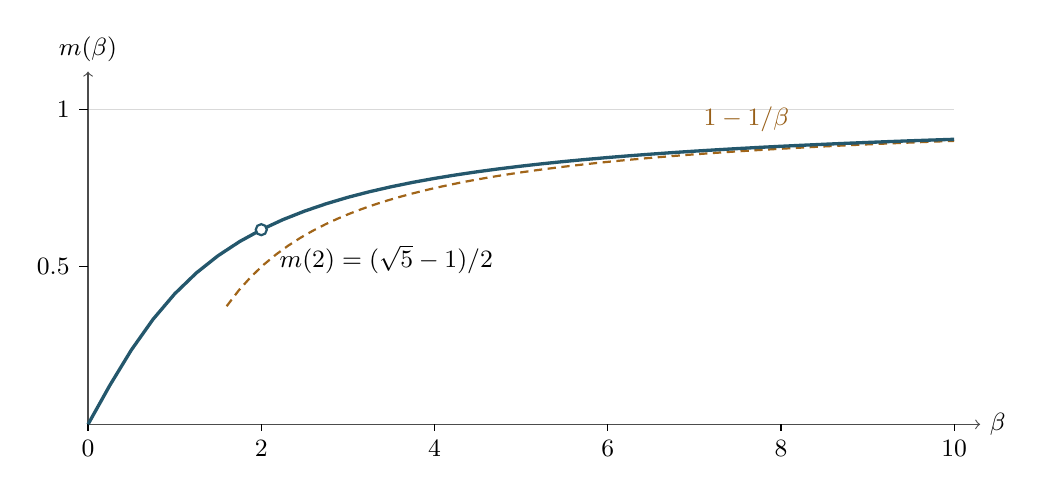
\begin{tikzpicture}[x=11mm,y=40mm,font=\small]
  \draw[black!15] (0,1)--(10,1);
  \draw[->,black!70] (0,0)--(10.3,0) node[right,text=black] {$\beta$};
  \draw[->,black!70] (0,0)--(0,1.12) node[above,text=black] {$m(\beta)$};
  \foreach \x in {0,2,4,6,8,10} \draw (\x,0)--++(0,-.02) node[below] {$\x$};
  \foreach \y in {0.5,1} \draw (0,\y)--++(-.1,0) node[left] {$\y$};
  \draw[glowgold!85!black,densely dashed,line width=.8pt,domain=1.6:10,samples=60] plot (\x,{1-1/\x});
  \draw[glowblue,line width=1.2pt] plot coordinates {
   (0,0.0000) (0.25,0.1231) (0.5,0.2361) (0.75,0.3333) (1,0.4142) (1.25,0.4806) (1.5,0.5352)
   (1.75,0.5803) (2,0.6180) (2.25,0.6499) (2.5,0.6770) (2.75,0.7004) (3,0.7208) (3.25,0.7386)
   (3.5,0.7543) (3.75,0.7683) (4,0.7808) (4.25,0.7920) (4.5,0.8022) (4.75,0.8114) (5,0.8198)
   (5.25,0.8275) (5.5,0.8346) (5.75,0.8411) (6,0.8471) (6.25,0.8527) (6.5,0.8579) (6.75,0.8628)
   (7,0.8673) (7.25,0.8715) (7.5,0.8755) (7.75,0.8793) (8,0.8828) (8.25,0.8861) (8.5,0.8892)
   (8.75,0.8922) (9,0.8950) (9.25,0.8977) (9.5,0.9003) (9.75,0.9027) (10,0.9050)};
  \filldraw[draw=glowblue,fill=white,line width=.8pt] (2,0.6180) circle[radius=2pt];
  \node[below right] at (2.1,0.6) {$m(2)=(\sqrt5-1)/2$};
  \node[text=glowgold!80!black] at (7.6,0.97) {$1-1/\beta$};
\end{tikzpicture}
\caption{Predicted energy curve $m(\beta)$ for a large Hadamard array (solid) and its low-temperature approximation $1-1/\beta$ (dashed).}\label{fig:energy}
\end{figure}

The program \texttt{freeenergy.py} checks the Catalan coefficients exactly through order 30 and evaluates the energy curve. The Taylor series for $\Phi_0(\beta^2/4)$ has radius 1 in $\beta$, from its branch points at $\beta=\pm i$. The coefficientwise limit alone does not establish convergence of the finite-array pressure at any fixed $\beta>0$. The weak-field dynamical instability of \cite{cfi} concerns relaxation, whereas this question concerns equilibrium at Hadamard couplings.

\medskip
\noindent\textbf{Fourier matrices and the next term.}
We now take $H=F_{\mathbb Z_q^n}$, with $q$ prime and $N=q^n$.
The Fourier sum of an individual graph is an exact power of $N$.
This determines the bottom degree of $C_k$ as well as its top degree.

\begin{samepage}
\begin{prop}\label{prop:free-fourier}
For fixed $q,k$, the coefficient $C_k(F_{\mathbb Z_q^n})$ is a polynomial in
$N=q^n$ of degree $k+1$ with lowest term
\[
 [N^2]C_k=w_k^2,\qquad w_k=k![t^k]\log f(t)
\]
in the notation of Section~\ref{sec:moments}. In particular its smallest
degree is exactly 2.
\end{prop}
\end{samepage}
\begin{proof}
For a connected graph with $r$ row vertices and $s$ column vertices, let
$M_{ij}$ be the number of plus edges minus the number of minus edges
between vertices $i,j$. With vertex labels in $\mathbb F_q^n$, summing
the row labels first gives
\[
 S_D(F_{\mathbb Z_q^n})=N^{r+s-\operatorname{rank}_q M}
\]
Indeed, character orthogonality imposes $M y=0$ independently in each
of the $n$ coordinates of the column labels $y$. This proves
polynomiality, and Theorem~\ref{thm:free-leading} gives the degree.
The row and column sums of $M$ are zero by balance, so its rank is at
most $\min(r-1,s-1)$. The exponent is at least $1+\max(r,s)$.
It equals 2 precisely for one row block and one column block.
This unique pair of partitions contributes $d_k^2/(k!)^2=w_k^2$.

For nonvanishing, write $b=f'/f=\sum_{j\geq0}b_jt^j$. The identity
$tf''+f'=f$ gives $b_0=1$ and
\[
 (j+1)b_j=-\sum_{h=0}^{j-1}b_h b_{j-1-h}\qquad(j\geq1)
\]
By induction $(-1)^j b_j>0$. Since $w_k=(k-1)!b_{k-1}$, the bottom
coefficient is positive.
\end{proof}

There is also a direct way to see which Fourier graphs reach degree
$k+1$. Orient plus edges from row to column and minus edges from column
to row. Balance and connectedness give an Euler tour. Along the tour the
Fourier exponent is the sum of $(u_{i_h}-u_{i_{h+1}})\cdot v_{j_h}$
over $1\leq h\leq k$, with $i_{k+1}=i_1$. Let $R,C$ record the visits, so that
column $h$ of $R$ is the coordinate vector indexed by $i_h$, and column
$h$ of $C$ is indexed by $j_h$. With $D z=(z_h-z_{h-1})_h$ in cyclic
order, we obtain
\[
 M=RDC^t,\qquad \operatorname{rank}_q M\geq r+s-k-1
\]
Here $D$ kills exactly the constants, which belong to the image of $C^t$.
Thus $D\operatorname{im} C^t$ has dimension $s-1$ and $\ker R$ has
dimension $k-r$. The rank reaches the displayed lower bound exactly when
$\ker R\subseteq D\operatorname{im} C^t$. The kernel is spanned by
$e_h-e_j$ for pairs of visits to the same row vertex. A cyclic primitive
of each such difference is the indicator of the interval from $h$ up to
but excluding $j$, up to an additive constant. It lies in
$\operatorname{im} C^t$ precisely when the interval is a union of whole
column blocks. This criterion for top degree is independent of $q$.

Write $C_k=\sum_{g=0}^{k-1}c_{k,g}N^{k+1-g}$ and
$\Phi_g(x)=\sum_{k\geq g+1}c_{k,g}x^k$. Regrouping powers of $N$ gives
\[
 \log G_H(x/N)=N\Phi_0(x)+\Phi_1(x)+\frac{\Phi_2(x)}N+\cdots
\]
coefficientwise in $x$. The function $\Phi_0$ is given by
Theorem~\ref{thm:free-leading}. The next series has a different
description in terms of vertices of degree 4.

\begin{samepage}
\begin{thm}\label{thm:free-odd}
For the Fourier matrices of $\mathbb Z_q^n$, the coefficient
\[
 [x^k]\Phi_1(x)=[N^k]C_k(F_{\mathbb Z_q^n})
\]
is the same for every odd prime $q$ and every fixed $k\geq1$.
Here the coefficient is zero at $k=1$. Thus the generic series $\Phi_1$
agrees to all orders with that of each odd prime.
\end{thm}
\end{samepage}
\begin{proof}
Apply the degree-2 reductions in the proof of
Theorem~\ref{thm:free-leading}. A completely reduced graph contributes
only at degree $k+1$. Otherwise, suppose that $k-m$ vertices were removed
and that the remaining graph has $2m$ edges and $v$ vertices. Its exact
contribution before multiplying by the graph weight is
\[
 N^{k-m+v-\operatorname{rank}_q M}
\]
with $M$ the signed edge-count matrix of the remaining graph.
Every remaining vertex has degree at least 4, so $v\leq m$.
Degree $k$ occurs exactly when $v=m$ and $M=0$ modulo $q$.
The first condition says that every vertex has degree 4. It therefore
has 2 edges of either sign, and every entry of $M$ is one of
$-2,-1,0,1,2$. For odd $q$, vanishing modulo $q$ is exactly integer
vanishing. Thus the very same pairs of partitions, with the same weights,
contribute at degree $k$ for every odd prime. The generic value follows
by stabilization at each fixed order from Theorem~\ref{thm:poly}.
\end{proof}

Characteristic 2 allows a pair of parallel edges with the same sign
to cancel in $M$ modulo 2. For instance, double the edges of a square,
with signs alternating around the square and equal within each pair.
Its signed edge-count matrix is
\[
 M=\begin{pmatrix}2&-2\\-2&2\end{pmatrix}
\]
of rank zero in characteristic 2 and rank one in every odd
characteristic. Figure~\ref{fig:free-square} shows the 2 possible kinds of
cancellation on a doubled square.

\begin{figure}[htb!]
\centering
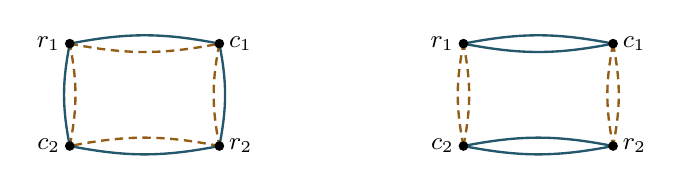
\begin{tikzpicture}[font=\small,
    plus/.style={draw=glowblue,line width=.85pt},
    minus/.style={draw=glowgold!78!black,densely dashed,line width=.85pt}]
  \foreach \offset/\paired in {0/0,5.0/1}{
    \begin{scope}[xshift=\offset cm]
      \coordinate (a) at (0,1.3); \coordinate (b) at (1.9,1.3);
      \coordinate (c) at (1.9,0); \coordinate (d) at (0,0);
      \foreach \u/\v/\parity in {a/b/0,b/c/1,c/d/0,d/a/1}{
        \ifnum\paired=0
          \draw[plus] (\u) to[bend left=11] (\v);
          \draw[minus] (\u) to[bend right=11] (\v);
        \else
          \ifnum\parity=0 \def\kind{plus}\else\def\kind{minus}\fi
          \draw[\kind] (\u) to[bend left=11] (\v);
          \draw[\kind] (\u) to[bend right=11] (\v);
        \fi
      }
      \foreach \v in {a,b,c,d} \fill (\v) circle[radius=1.75pt];
      \node[left] at (a) {$r_1$}; \node[right] at (b) {$c_1$};
      \node[right] at (c) {$r_2$}; \node[left] at (d) {$c_2$};
    \end{scope}
  }
\end{tikzpicture}
\caption{A solid edge carries a plus sign and a dashed edge a minus sign.
On the left the signed counts cancel over the integers. On the right
they cancel modulo 2.}\label{fig:free-square}
\end{figure}

The difference is already visible in the first
matrix-dependent moment. By Theorem~\ref{thm:s2} all lower moments
agree, and the difference at the 8th moment is $18S_2(W_N)$ relative
to the generic polynomial. Consequently
\[
 C_4^{Walsh}(N)-C_4^\infty(N)
 =\frac{18}{(4!)^2}\,N^3(N-1)=\frac{N^4-N^3}{32}
\]
as a polynomial identity. This gives the first difference of the 2
series $\Phi_1$, namely $x^4/32$. The program \texttt{graphcheck.py}
enumerates the connected graphs of Lemma~\ref{lem:connected-free} for
$k\leq4$, over the fields with 2, 3 and 5 elements, and checks the top and
bottom coefficients, the agreement of the degree $k$ terms for $q=3,5$,
and this Walsh difference.

The coefficients calculated by \texttt{logexp.py} through $k=8$ give
\[
 \Phi_1^{odd}(x)=\frac{x^2}{4}-x^3+\frac{15}{4}x^4-14x^5
 +\frac{629}{12}x^6-197x^7+\frac{5945}{8}x^8+O(x^9)
\]
For Walsh the coefficients of $x^4,x^5,x^6$ are
$121/32,-57/4,3443/64$. For an odd prime $q$, the data suggest a first
departure from the generic series at $g=q-1$, beginning with the term
$x^{2q}$ in $\Phi_{q-1}$. The theorem proves the agreement at $g=1$.

The formula for $\Phi_0$ also gives
$\Phi_0(\beta^2/4)/\beta\to1$ as $\beta\to\infty$. This agrees with the
bound $|\Omega|\leq N^{3/2}$, attained for $W_N$ with $N=4^m$ by taking
$b$ to be the sign vector of a bent function \cite{rot} and choosing
$a$ to align the row sums. To use the formal calculation at fixed
temperature we still need control as $k$ grows.

\begin{samepage}
\begin{question}\label{que:free}
Can the connected graphs with remaining vertices of degree 4 be summed
to give closed forms for $\Phi_1$ in odd characteristic and for Walsh?
At which $g$ and which power of $x$ does each odd prime first differ from
the generic expansion? For which fixed inverse temperatures $\beta>0$ does
\[
 \frac1N\log G_H\big(\beta^2/(4N)\big)\longrightarrow\Phi_0(\beta^2/4)
\]
hold uniformly over complex Hadamard matrices, and can this convergence
give the estimates near the edge in Section~\ref{sec:edge}? At the Fourier point $\alpha=1$, what is the relation between equilibrium behavior and the relaxation dynamics?
\end{question}
\end{samepage}

\section{Ground states and bistochastic forms}\label{sec:edge}

\noindent\textbf{Crystals and glasses.}
In a periodic frustrated system the configurations selected by cooling can differ from the absolute energy minimizers. Chandra, Feigel'man, Ioffe and Kagan discuss this distinction for their crossed-wire model \cite{cfk}. For every Hadamard array we can identify the exact ground states by $a=Hb/\sqrt N$. Determining the barriers and relaxation times between configurations requires further information about $H$ and the dynamics. Figure~\ref{fig:landscape} illustrates the distinction.

\begin{figure}[htb!]
\centering
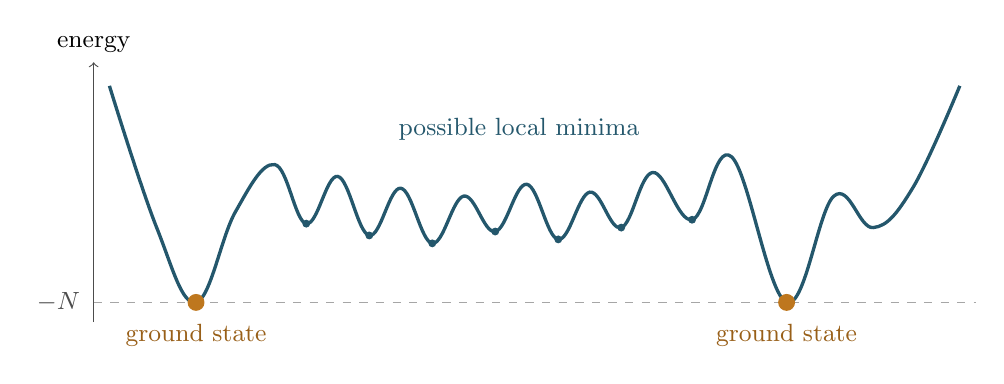
\begin{tikzpicture}[x=10mm,y=10mm,font=\small]
  \draw[->,black!70] (-.2,0)--(-.2,3.3) node[above,text=black] {energy};
  \draw[black!35,dashed] (-.2,.25)--(11,.25);
  \node[left,text=black!70] at (-.25,.25) {$-N$};
  \draw[glowblue,line width=1.2pt] plot[smooth,tension=.65] coordinates {
    (0,3) (.6,1.2) (1.1,.25) (1.6,1.4) (2.1,2.0) (2.5,1.25) (2.9,1.85) (3.3,1.1) (3.7,1.7)
    (4.1,1.0) (4.5,1.6) (4.9,1.15) (5.3,1.75) (5.7,1.05) (6.1,1.65) (6.5,1.2) (6.9,1.9)
    (7.4,1.3) (7.9,2.1) (8.6,.25) (9.2,1.6) (9.7,1.2) (10.2,1.7) (10.8,3)};
  \filldraw[glowgold] (1.1,.25) circle[radius=.1];
  \filldraw[glowgold] (8.6,.25) circle[radius=.1];
  \node[below,text=glowgold!80!black] at (1.1,.1) {ground state};
  \node[below,text=glowgold!80!black] at (8.6,.1) {ground state};
  \node[text=glowblue] at (5.2,2.45) {possible local minima};
  \foreach \x/\y in {2.5/1.25,3.3/1.1,4.1/1.0,4.9/1.15,5.7/1.05,6.5/1.2,7.4/1.3}
    \fill[glowblue] (\x,\y) circle[radius=.05];
\end{tikzpicture}
\caption{A schematic landscape distinguishes global minima of energy $-N$ from possible higher local minima. Only the global minimum value is prescribed by the Hadamard condition.}\label{fig:landscape}
\end{figure}

\medskip
\noindent\textbf{Idel--Wolf.} By \cite{iwo}, conjectured in \cite{dvb}, any unitary matrix can be written as $LAR$, with $L,R$ diagonal unitaries and $A$ having all row and column sums equal to 1. The proof is non-constructive, and relies on the non-displaceability of the Clifford torus \cite{bep}. For a complex Hadamard matrix this means that $H$ is equivalent to a bistochastic matrix, with all row and column sums $\lambda$, $|\lambda|=\sqrt N$. In glow terms, $|\Omega|$ is the excess of the equivalent matrix $D_{\bar a}HD_b$, that is, the modulus of the sum of its entries, and the Cauchy--Schwarz bound $|\Omega|\leq N^{3/2}$ is attained, the maximizers being exactly the bistochastic forms. In the real case, the maximal excess of the real Hadamard matrices is a classical topic \cite{bes,fko,kha}, the bound $N^{3/2}$ being attained precisely by the regular Hadamard matrices, which exist only when $N$ is a square. In the complex case, Idel--Wolf gives:
$$\lim_{p\to\infty}\big[E(|\Omega|^{2p})\big]^{\frac1p}=N^3$$

For $F_2$ we can see the maximizers directly. Take $b=(1,e^{it})$ after
removing its common phase. Choosing the 2 phases of $a$ to align the
terms of $\langle F_2b,a\rangle$ gives
\[
 \max_a |\Omega|=|1+e^{it}|+|1-e^{it}|=2\big(|\cos(t/2)|+|\sin(t/2)|\big)
\]
so the bound $2\sqrt2$ is attained precisely where the 2 summands
$|1+e^{it}|$ and $|1-e^{it}|$ agree, as in Figure~\ref{fig:edge}.

\begin{figure}[H]
\centering
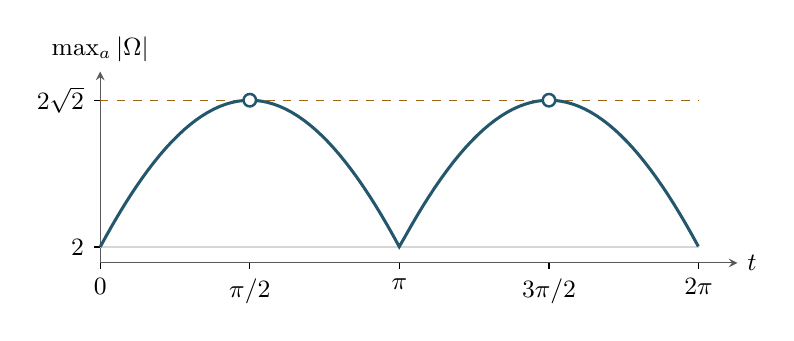
\begin{tikzpicture}[x=3.8cm,y=2.25cm,font=\small,>=stealth]
  \draw[->,black!65] (0,1.91)--(2.13,1.91) node[right,text=black] {$t$};
  \draw[->,black!65] (0,1.91)--(0,2.99) node[above,text=black] {$\max_a|\Omega|$};
  \draw[glowgold!85!black,dashed] (0,{2*sqrt(2)})--(2,{2*sqrt(2)});
  \draw[black!16] (0,2)--(2,2);
  \foreach \x/\tick in {0/0,.5/{\pi/2},1/\pi,1.5/{3\pi/2},2/{2\pi}}
    \draw (\x,1.91)--++(0,-.032) node[below] {$\tick$};
  \draw (0,2)--++(-.022,0) node[left] {$2$};
  \draw (0,{2*sqrt(2)})--++(-.022,0) node[left] {$2\sqrt2$};
  \draw[glowblue,line width=1.1pt,samples=101,domain=0:2,variable=\x]
    plot (\x,{2*(abs(cos(90*\x))+abs(sin(90*\x)))});
  \foreach \x in {.5,1.5}
    \filldraw[draw=glowblue,fill=white,line width=.9pt]
      (\x,{2*sqrt(2)}) circle[radius=2.25pt];
\end{tikzpicture}
\caption{The edge for $F_2$. The 2 peaks correspond to $b=(1,i)$ and
$b=(1,-i)$, up to a common phase.}\label{fig:edge}
\end{figure}

\medskip

\noindent\textbf{An asymptotic version.} Idel--Wolf gives the location of the edge exactly. The volume of configurations near it is a different question. Suppose that along a sequence of Hadamard matrices the pressure converges at every fixed $\beta\ge0$ to $\Lambda(\beta)=\Phi_0(\beta^2/4)$. Rotation invariance gives the limiting logarithmic moment generating function $\Lambda(|t|)$ for the two real coordinates of $\Omega/N^{3/2}$, with speed $N$ and $t\in\mathbb R^2$. This function is finite and differentiable everywhere, including at the origin. The G\"artner--Ellis theorem \cite{dez} gives a radial rate function. At radius $0\le r<1$ its maximizer satisfies $r=\Lambda'(\beta)$, or $\beta=2r/(1-r^2)$, so
\[
 I(r)=\sup_{\beta\ge0}\{\beta r-\Lambda(\beta)\}=-\log(1-r^2)
\]
The rate is infinite for $r\ge1$. Since it is continuous and increasing below 1, the open and closed large deviation bounds agree at every threshold $1-\varepsilon$, $0<\varepsilon<1$. Under the stated pressure hypothesis,
\[
 \lim_{N\to\infty}\frac1N\log P\big[|\Omega|\ge(1-\varepsilon)N^{3/2}\big]
       =\log(2\varepsilon-\varepsilon^2)
\]
These configurations are almost bistochastic in mean square. Indeed the vector $R$ of row sums of $D_{\bar a}HD_b$ satisfies $\min_\theta\|R-\sqrt N e^{i\theta}1\|^2=2N^2-2\sqrt N|\Omega|$. A possible route to the pressure hypothesis is a large deviation estimate for the empirical law of $|(Hb)_j|/\sqrt N$, in the spirit of spherical integrals \cite{gma}, with phase vectors constrained to the torus.

\medskip

\noindent\textbf{The edge at fixed order.}
Let $a,b$ be independent Haar vectors in $\mathbb T^N$. For a complex
Hadamard matrix $H$, we use the normalization
\[
 U=H/\sqrt N,\qquad M_p(H)=E\left[\left(\frac{|\langle Hb,a\rangle|^2}{N^3}\right)^p\right],
 \qquad Y(b)=\frac1N\sum_{j=1}^N|(Ub)_j|
\]
The largest value of $|\langle Hb,a\rangle|/N^{3/2}$ for fixed $b$ is $Y(b)$.
If $r_j=|(Ub)_j|$, then $\sum_j r_j^2=N$, and hence
\[
 1-Y(b)=\frac{1}{2N}\sum_{j=1}^N(r_j-1)^2
\]
In particular, $Y=1$ precisely at the bi-unimodular vectors of $U$.
For the cyclic Fourier matrix these give the first rows of the circulant
complex Hadamard matrices and correspond to unimodular cyclic $N$-roots
\cite{bjo,haa}. For $N$ prime the total number of cyclic $N$-roots over
$\mathbb C$, counted with multiplicity, is $\binom{2N-2}{N-1}$ by
\cite{haa}. Only the unimodular solutions enter the glow. The same
maximizers appear at the cold end of the Villain model in
Section~\ref{sec:general}.

Fourier ground states also occur in signal design. For a unimodular periodic input $b$, the discrete Fourier transform of its periodic autocorrelations gives $|(F_Nb)_j|^2$, up to the choice of sign in the transform. The zero-shift correlation is $N$. The nonzero-shift correlations vanish precisely when $|(F_Nb)_j|=\sqrt N$ for every $j$. In radar a pulse with these correlations separates its delay from all other cyclic shifts. The polyphase codes of \cite{fza,chu} give explicit examples. For Chu's choice $b_k=e^{-\pi ik(k+1)/N}$ at odd $N$ and $b_k=e^{-\pi ik^2/N}$ at even $N$, the sequence is periodic and $b_{k+h}\bar b_k$ is a constant in $k$ times $e^{-2\pi ihk/N}$. Summing over $k$ proves the cancellation for each nonzero shift. There are other inputs: at $N=4$, every $b=(1,z,1,-z)$ with $|z|=1$ qualifies. In each case the ground-state partner is $a=F_Nb/\sqrt N$. Figure~\ref{fig:chu} compares the output moduli of a random input and a Chu input. The program \texttt{chu.py} checks the Chu formulas for $2\le N\le64$.

\begin{figure}[htb!]
\centering
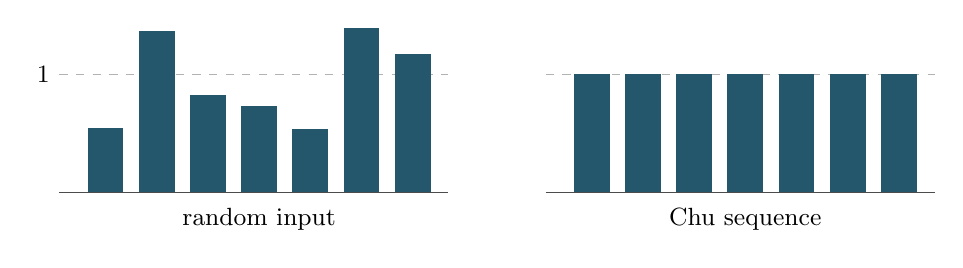
\begin{tikzpicture}[x=6.5mm,y=15mm,font=\small]
  \foreach \shift/\vals/\name in {0/{0.545,1.370,0.827,0.731,0.536,1.396,1.171}/random input,
                                  9.5/{1,1,1,1,1,1,1}/Chu sequence}{
    \begin{scope}[shift={(\shift,0)}]
      \draw[black!30,dashed] (-.4,1)--(7.2,1);
      \foreach \v [count=\i from 0] in \vals
        \fill[glowblue] (\i+.15,0) rectangle (\i+.85,\v);
      \draw[black!70] (-.4,0)--(7.2,0);
      \node[below] at (3.5,-.05) {\name};
    \end{scope}}
  \node[left] at (-.4,1) {$1$};
\end{tikzpicture}
\caption{Normalized moduli $|(F_7b)_j|/\sqrt7$ for a random input (left) and a Chu input (right). A flat output at height 1 gives a ground-state partner.}\label{fig:chu}
\end{figure}

\begin{samepage}
\begin{question}\label{que:laplace}
What is the leading asymptotic of $M_p(H)$ as $p\to\infty$ for the Walsh
matrices $W_N$ with $N\geq8$, and for the real Hadamard matrices of order
$16$? Which families of bi-unimodular vectors, or which intersections of
these families, determine the exponent and leading constant?
\end{question}
\end{samepage}

We first explain how the alternating phase iteration of \cite{dvb,frz}
finds these maximizers locally. The phase map $ph(z)=z/|z|$ is taken
in each coordinate.

\begin{samepage}
\begin{thm}\label{thm:iteration}
For every unitary $U$ and every bi-unimodular vector $b_*$, the iteration
\[
 b_{k+1}=ph\big(U^*ph(Ub_k)\big)
\]
is well defined and converges to a bi-unimodular vector for every $b_0$
in some neighborhood of $b_*$ in $\mathbb T^N$. In particular the set of
successful starting points has positive Haar measure.
\end{thm}
\end{samepage}
\begin{proof}
Regard $A=\mathbb T^N$ and $B=U^*\mathbb T^N$ as subsets of
$\mathbb R^{2N}$. A point of $A\cap B$ is exactly a bi-unimodular vector.
Near these tori their Euclidean nearest-point projections are
\[
 P_A z=ph(z),\qquad P_B z=U^*ph(Uz)
\]
Thus one full step on $A$ is $P_A P_B$. Both sets are closed real
algebraic manifolds. The torus has positive reach: every point at
distance less than one from it has all coordinates nonzero and a unique
nearest point. Its unitary image has the same property. Corollary~9 of
Noll and Rondepierre \cite{nor} therefore gives a neighborhood of each
intersection point in which starting alternating projections converge to
some point of the intersection. The limit can depend on $b_0$.

For the phase conventions, shrink the neighborhood so that $d(b_0,B)<1$.
The distances between successive projections are nonincreasing. Each
projection is therefore taken at distance less than one and uses only
nonzero coordinates. Finally, Idel--Wolf \cite{iwo} gives at least one
intersection point for every unitary $U$, and every relatively open
neighborhood in $A$ has positive Haar measure.
\end{proof}

For $U=H/\sqrt N$, the positive scalar cancels from both phase maps.
The size of the basin and the question of convergence from Haar-almost
every starting point remain to be investigated.

\medskip
\noindent\textbf{Alignment of the output phases.}
To compute edge moments, we first integrate out $a$. This contributes a
Gaussian factor even when the maximizing set in the $b$ variables is singular.

\begin{samepage}
\begin{lem}\label{lem:edge-align}
Put $d=N-1$ and $q_j=r_j/\sum_i r_i$. For fixed $b$ we have
\[
 E_a\left[\left(\frac{|\langle Hb,a\rangle|^2}{N^3}\right)^p\right]
 =Y(b)^{2p}\,\frac{p^{-d/2}}{2^d\pi^{d/2}\sqrt{\prod_j q_j}}\,(1+o(1))
\]
as $p\to\infty$, uniformly for $q$ in compact subsets of the open
probability simplex. In particular the prefactor multiplying
$Y(b)^{2p}p^{-d/2}$ tends to $N^{N/2}/(2^d\pi^{d/2})$ at the edge.
\end{lem}
\end{samepage}
\begin{proof}
After aligning the arguments of $(Ub)_j$ and dividing by a common
phase, the integral left after extracting $Y^{2p}$ is the Haar average
of $|\sum_jq_j e^{it_j}|^{2p}$ with $t_N=0$. For positive weights its
unique maximum is $t=0$. The quadratic part of its squared-modulus
deficit is
\[
 \sum_{i<j}q_iq_j(t_i-t_j)^2
  =\sum_{j<N}q_jt_j^2-\Big(\sum_{j<N}q_jt_j\Big)^2
\]
The matrix determinant lemma gives determinant $\prod_{j=1}^N q_j$.
Gaussian integration with Haar density $(2\pi)^{-d}$ gives the formula.
On a compact set of positive weights the quadratic forms have a common
positive lower bound on the unit sphere, and the squared modulus is
uniformly below one away from $t=0$. These bounds give uniformity.
At $Y=1$ all the $q_j$ are $1/N$.
\end{proof}

For example, suppose the maxima of $Y$ are isolated and nondegenerate
after fixing $b_N=1$. At each such $b_*$ write
$1-Y(b_*e^{it})^2=t^t K_* t+O(|t|^3)$ in the $d$ relative angles
($t_N=0$, with entrywise multiplication). A second Gaussian integration
now gives the precise isolated-maximizer formula
\[
 M_p(H)\sim \frac{N^{N/2}}{(4\pi)^{N-1}}\,
 p^{-(N-1)}\sum_{b_*}\frac{1}{\sqrt{\det K_*}}
\]
The sum is finite by compactness. Already for the Walsh matrix of order
4 a different local calculation is needed.

\begin{samepage}
\begin{thm}\label{thm:walsh-edge}
For the 2 smallest nontrivial Walsh matrices we have
\[
 M_p(W_2)\sim\frac{2}{\pi p},\qquad
 M_p(W_4)\sim\frac{2\sqrt2\,\Gamma(1/4)^3}{\pi^{9/2}}\,p^{-9/4}
\]
as $p\to\infty$. For $W_4$ the leading term comes from the crossings of
the maximizing families.
\end{thm}
\end{samepage}
\begin{proof}
For $W_2=F_2$, Figure~\ref{fig:edge} gives
$Y(t)=(|\cos(t/2)|+|\sin(t/2)|)/\sqrt2$. Its 2 maxima are at
$t=\pi/2,3\pi/2$. At either one $1-Y(t)^2=(t-t_*)^2/4+O((t-t_*)^4)$,
so the preceding formula gives $2/(\pi p)$.

For $W_4$, index the coordinates by signs $s,t\in\{-1,1\}$ and write
\[
 b_{s,t}=e^{i(D+sA+tB+stC)},\qquad
 u=\cos(2A),\quad v=\cos(2B),\quad w=\cos(2C)
\]
Independent uniform angles $D,A,B,C$ give Haar $b$. Indeed the integer
matrix taking these angles to the 4 coordinate angles has nonzero
determinant, so its map on tori is onto and preserves Haar probability.
Consequently $u,v,w$ are independent with density
$1/(\pi\sqrt{1-u^2})$ on $(-1,1)$.

The 3 nonconstant normalized Walsh coefficients of $r^2$, taken
entrywise, are $uv,uw,vw$ in some order. To see this, for each nontrivial
group element $h$ the coefficient is
$\frac14\sum_g b_g\bar b_{gh}$ by character orthogonality.
For example, changing $s$ to $-s$ and averaging over $s,t$ gives $uw$.
The constant coefficient is one. Parseval therefore gives
\[
 Q(u,v,w)=u^2v^2+u^2w^2+v^2w^2=\frac14\sum_{j=1}^4(r_j^2-1)^2
\]
The maximizing set is the union of the 3 coordinate axes in this
cube. Figure~\ref{fig:walsh-cross} shows 2 slices near the crossing. Since $0\le r_j\le2$, the
identity for $1-Y$ above shows that $1-Y^2\ge cQ$ everywhere for some
$c>0$. Near $Q=0$, all $r_j$ tend uniformly to one, so
\[
 1-Y^2=\big(\tfrac14+o(1)\big)Q
\]
by factoring $r_j^2-1=(r_j-1)(r_j+1)$.

\begin{figure}[H]
\centering
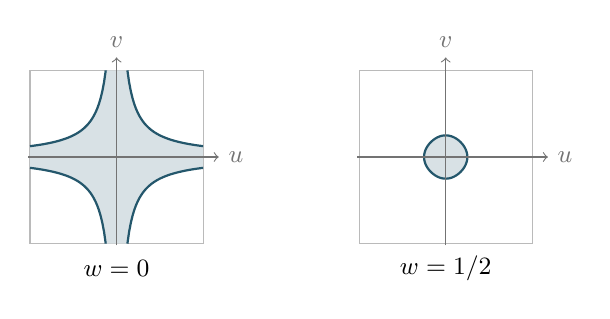
\begin{tikzpicture}[x=1.1cm,y=1.1cm,font=\small]
\foreach \offset/\zval in {0/0,3.8/.5}{
 \begin{scope}[shift={(\offset,0)}]
  \draw[black!27] (-1,-1) rectangle (1,1);
  \begin{scope}
  \clip (-1,-1) rectangle (1,1);
  \ifdim\zval pt=0pt
   \fill[glowblue!18] (-1,.125)
    -- plot[domain=-1:-.125,samples=45] (\x,{-.125/\x})
    -- (.125,1) -- plot[domain=.125:1,samples=45] (\x,{.125/\x})
    -- (1,-.125) -- plot[domain=1:.125,samples=45] (\x,{-.125/\x})
    -- (-.125,-1) -- plot[domain=-.125:-1,samples=45] (\x,{.125/\x}) -- cycle;
   \foreach \xs in {-1,1}\foreach \ys in {-1,1}
    \draw[glowblue,thick] plot[domain=.125:1,samples=45] ({\xs*\x},{\ys*.125/\x});
  \else
   \filldraw[draw=glowblue,thick,fill=glowblue!18]
    plot[domain=0:360,samples=121]
    ({.25*cos(\x)},{.25*sin(\x)/sqrt(1+.25*cos(\x)^2)}) -- cycle;
  \fi
  \end{scope}
  \draw[->,black!55] (-1.02,0)--(1.18,0) node[right] {$u$};
  \draw[->,black!55] (0,-1.02)--(0,1.15) node[above] {$v$};
  \ifdim\zval pt=0pt
   \node at (0,-1.29) {$w=0$};
  \else
   \node at (0,-1.29) {$w=1/2$};
  \fi
 \end{scope}
}
\end{tikzpicture}
\caption{2 slices of $Q(u,v,w)\le1/64$ for $W_4$, drawn on the same
scale. At $w=0$ the maximizing set contains both axes in the slice.
At $w=1/2$ its only point is the origin of the slice.}\label{fig:walsh-cross}
\end{figure}

Fix a small cube $|u|,|v|,|w|<\delta$ about the origin. On its complement,
if $|u|\ge\delta$ then $Q\ge\delta^2(v^2+w^2)$, and likewise for the
other coordinates. The arcsine average of $e^{-cp v^2}$ is $O(p^{-1/2})$:
its density is bounded near zero and its integral away from zero is
exponentially small. The complement thus contributes $O(p^{-1})$ to
$E_b Y^{2p}$. Inside the cube put $(u,v,w)=p^{-1/4}(x,y,z)$.
The 3 densities tend to $1/\pi$ each, and the rescaled integrand
is bounded by a constant times $e^{-cQ(x,y,z)}$. For the limiting integral
we have
\[
 \int_{\mathbb R^3}e^{-Q(x,y,z)/4}\,dx\,dy\,dz
 =4\left(\int_0^\infty h^{-1/2}e^{-h^2/4}\,dh\right)^3
 =\sqrt2\,\Gamma(1/4)^3
\]
Indeed, on the positive octant the substitution $(l,m,n)=(xy,yz,zx)$
has inverse Jacobian $1/(2\sqrt{lmn})$. This also proves integrability
for every $c>0$ by rescaling. Dominated convergence gives
\[
 E_b Y^{2p}\sim \frac{\sqrt2\,\Gamma(1/4)^3}{\pi^3}\,p^{-3/4}
\]
For the final integration restrict first to $Y$ close to one, where
Lemma~\ref{lem:edge-align} is uniform. The complementary contribution is
exponentially small since the conditional moment is bounded by $Y^{2p}$.
As the neighborhood of the edge shrinks, the alignment prefactor tends
uniformly to $2/\pi^{3/2}$. Multiplication by $(2/\pi^{3/2})p^{-3/2}$
gives the stated constant and exponent.
\end{proof}

These asymptotics are confirmed numerically by the program
\texttt{walshedge.py}. For $W_2$ the program evaluates an exact finite sum numerically, and
$pM_p(W_2)$ agrees with $2/\pi$ to 8 digits at $p=10^5$. For $W_4$ the 2
factors are checked separately. Quadrature in $u,v,w$ gives
$E_bY^{2p}$ within $3\cdot10^{-5}$ of the predicted value at $p=10^8$, in
relative terms, and the exact moments of $\sum_{j=1}^4a_j$ give the
alignment constant $2/\pi^{3/2}$.

\medskip
\noindent\textbf{The low-temperature partition function at fixed size.}
Put $r=|\Omega|/N^{3/2}$ and $t=N\beta$. If $M_p=E(r^{2p})\sim C p^{-\gamma}$, then
\[
 \mathcal Z_H(\beta)\sim \frac{2^\gamma C}{\sqrt{2\pi}}\,
               e^{N\beta}(N\beta)^{-\gamma-1/2}
 \qquad(\beta\to\infty)
\]
Indeed, monotonicity between successive integer moments gives $E(r^t)\sim C(t/2)^{-\gamma}$. Near $r=1$, for each $0<\delta<1$, we have $r^t\le e^{-t(1-r)}\le r^{(1-\delta)t}$. Away from 1 all three terms are exponentially small. Letting $\delta\downarrow0$ gives the same equivalent for $E(e^{-t(1-r)})$. Rotation invariance gives $\mathcal Z_H=E[I_0(tr)]$, with the same circle average as in Section~\ref{sec:glow}. Laplace's formula at $\theta=0$ gives $I_0(x)\sim e^x/\sqrt{2\pi x}$. On $r\ge1-\delta$ this equivalent is uniform as $t\to\infty$, and $r^{-1/2}$ tends uniformly to 1 as $\delta\downarrow0$. The complement is exponentially smaller. Thus the powers of $N\beta$ in the denominator are $3/2$ for $W_2$ and $11/4$ for $W_4$. The extra $1/2$ in each case comes from aligning the overall phase of the glow with the real energy axis. For $W_2$ direct quadrature in \texttt{walshedge.py} gives $0.50799$ for $e^{-2\beta}(2\beta)^{3/2}\mathcal Z_{W_2}(\beta)$ at $\beta=10^4$, against the limiting constant $4/(\pi\sqrt{2\pi})=0.50795\ldots$.

\medskip
\noindent\textbf{The 5 real matrices of order 16.}
We use the representatives \texttt{had.16.0} through \texttt{had.16.4}
from \href{https://neilsloane.com/hadamard/index.html}{Sloane's library
of Hadamard matrices}. A dephased input has $b_1=1$. The table counts
inputs attaining $Y=1$, so each input determines its aligning output up
to a common phase.
\begin{center}
\begin{tabular}{lrr}
\toprule
Representative & Sign inputs & Fourth-root inputs\\
\midrule
\texttt{16.0} (Walsh) & 448 & 200704\\
\texttt{16.1} & 192 & 36864\\
\texttt{16.2} & 64 & 4096\\
\texttt{16.3} & 0 & 0\\
\texttt{16.4} & 0 & 0\\
\bottomrule
\end{tabular}
\end{center}
The square relation between the 2 columns follows from real
orthogonality and the arithmetic of the integer $32$.

\begin{samepage}
\begin{prop}\label{prop:edge-sixteen}
For any real Hadamard matrix of order $16$, dephased fourth-root
maximizers are in bijection with ordered pairs of dephased sign
maximizers. For the first 3 matrices in the table we have
\[
 M_p(H)\ge c_H p^{-45/4}
\]
for some $c_H>0$ and all sufficiently large $p$. The last 2
representatives have identical glow laws.
\end{prop}
\end{samepage}
\begin{proof}
For the first column encode each row of $H$ as a 16-bit integer $h_j$,
with a one at each minus sign and the first entry in the most significant
bit. A sign input is encoded by $m$ in the same way. The condition $b_1=1$
is $0\le m<2^{15}$. The $j$th row sum is $16-2d(m,h_j)$, where $d$
counts differing bits. Thus the exact count, in the order used above, is
\[
 \sum_{m=0}^{2^{15}-1}\prod_{j=1}^{16}
 {\bf1}_{\{6,10\}}\big(d(m,h_j)\big)
\]
The program \texttt{order16.py} evaluates this sum for the five matrices and checks the transpose relation used below.

Every fourth-root input has a unique expression $b=(s+it)/(1+i)$
with $s,t$ sign vectors. Dephasing fixes $s_1=t_1=1$. The equation
$|(Hb)_j|=4$ is equivalent to
\[
 (Hs)_j^2+(Ht)_j^2=32
\]
The only pair of integer squares with this sum is $16,16$. Thus both
$s$ and $t$ must be sign maximizers, and every ordered pair works.
For distinct dephased inputs $s,t$, the vectors $s\cos\theta+it\sin\theta$
give a nonconstant curve of maximizers after dephasing by $e^{-i\theta}$.

To obtain the lower bound, start at a sign maximizer $s$ and perturb
its 15 relative phases by $|t_j|\le p^{-1/4}$. Since $U=H/4$ is real
and $(Us)_j=\pm1$, the linear perturbation of each $(Us)_j$ is purely
imaginary. Uniformly in this box, $r_j=1+O(p^{-1/2})$ and hence
$1-Y=O(p^{-1})$. In particular, $Y^{2p}$ is bounded below by a positive
constant for large $p$. The box has Haar measure of order $p^{-15/4}$.
Lemma~\ref{lem:edge-align} supplies a further factor of order $p^{-15/2}$,
giving $p^{-45/4}$.

Finally, \texttt{had.16.4} is the transpose of \texttt{had.16.3},
as is seen entry by entry in the listed representatives. For a real
matrix, $\langle H^t b,a\rangle=\overline{\langle Ha,b\rangle}$.
Exchanging the independent inputs and using rotation invariance of the
glow proves equality in law.
\end{proof}

The exact exponents in order $16$ remain open. For the last 2
representatives, existence follows from \cite{iwo}, while the zero
counts force every dephased maximizing input to use at least one phase
outside the fourth roots of unity.

\section{Villain chains and gauge stiffness}\label{sec:villain}

So far the wires interacted only through the junctions. We now let neighboring parallel wires interact as well. Bend each layer into a cylinder, so that the row wires form a cycle, the wire $j$ being next to the wires $j\pm1$ modulo $N$, and similarly for the column wires. Then couple neighboring wires of the same layer by Villain bonds of stiffness $l$, defined below, as in Figure~\ref{fig:rings}.

\begin{figure}[H]
\centering
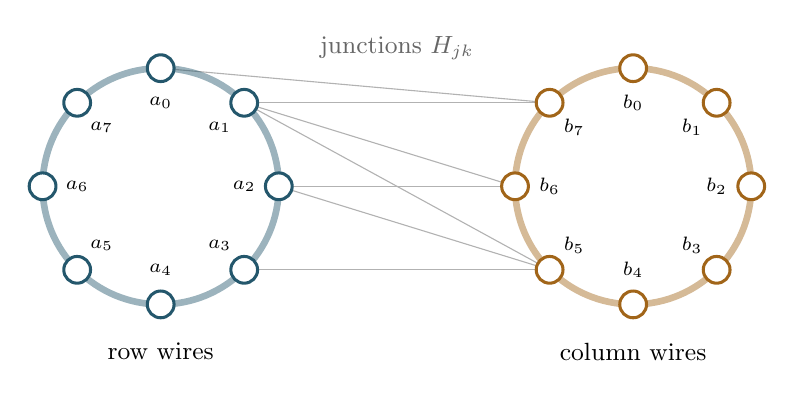
\begin{tikzpicture}[x=10mm,y=10mm,font=\small]
  \foreach \i/\k in {1/7,1/6,1/5,0/7,2/6,2/5,3/5}
    \draw[black!30] ({90-45*\i}:1.5)--($(6,0)+({90-45*\k}:1.5)$);
  \foreach \cx/\col/\lab/\name in {0/glowblue/a/row wires,6/glowgold!85!black/b/column wires}{
    \begin{scope}[shift={(\cx,0)}]
      \draw[\col,line width=2.4pt,opacity=.45] (0,0) circle[radius=1.5];
      \foreach \i in {0,...,7}{
        \filldraw[draw=\col,fill=white,line width=1.1pt] ({90-45*\i}:1.5) circle[radius=.17];
        \node at ({90-45*\i}:1.06) {\scriptsize $\lab_\i$};
      }
      \node at (0,-2.1) {\name};
    \end{scope}}
  \node[text=black!60] at (3,1.75) {junctions $H_{jk}$};
\end{tikzpicture}
\caption{The 2 layers, each bent into a cycle, with Villain bonds of stiffness $l$ between neighboring wires of the same layer (thick circles). A few of the $N^2$ junctions between the layers are drawn. At zero junction coupling and $l=0$ the wire phases are independent.}\label{fig:rings}
\end{figure}

With the coupling between layers switched off, $a$ and $b$ are independent periodic Villain chains. Write $E_l$ for expectation under this product law and put
\[
 Z=\langle Hb,a\rangle/N,\qquad E_H=-\sqrt N\,Re(Z)
\]
The law of $Z$ is the Villain glow. Let $\mathcal Z_{H,l}(\beta)$ denote the partition function when we multiply the two chain weights by $e^{-\beta E_H}$. The chain laws are invariant under independent global rotations, so phase averaging gives the exact expansion
\[
 \frac{\mathcal Z_{H,l}(\beta)}{\mathcal Z_{H,l}(0)}
 =E_l\big[e^{\beta\sqrt N\,Re(Z)}\big]
 =\sum_{p\ge0}\frac{E_l(|Z|^{2p})}{(p!)^2}
             \left(\frac{N\beta^2}{4}\right)^p
\]
It is this expansion in junction strength, at fixed bond stiffness $l$, whose coefficients we study.

In the absence of same-layer bonds, $Z$ is the normalized entry sum of the random rephasing $D_{\bar a}HD_b$, and its law is independent of the chosen representative. The new bonds have zero preferred phase difference. They fix a reference for relative phases along each cycle. Rephasing $H$ alone can now change fluxes around loops containing these bonds, and the cyclic order of the wires matters. Transforming the phases on \emph{all} links together still preserves the physics. At fixed $N$, as $l\to\infty$ the two chains each align up to one global phase, giving a uniform phase times the normalized entry sum of $H$.

We start with the Fourier matrix, labeling the rows and columns by $G=\mathbb Z_N$ in their natural cyclic order. For the higher-order fluctuations of the independent glow, and their dependence on the underlying finite abelian group, see \cite{banica}.

\medskip

\noindent\textbf{From a spin to a Gibbs measure.} 
At each site $j$ of the cycle place a unit vector in the plane, written
as $a_j=e^{i\theta_j}$. Angles differing by $2\pi$ give the same spin.
Figure~\ref{fig:spins} shows how to read the angle across one bond.

\begin{figure}[H]
\centering
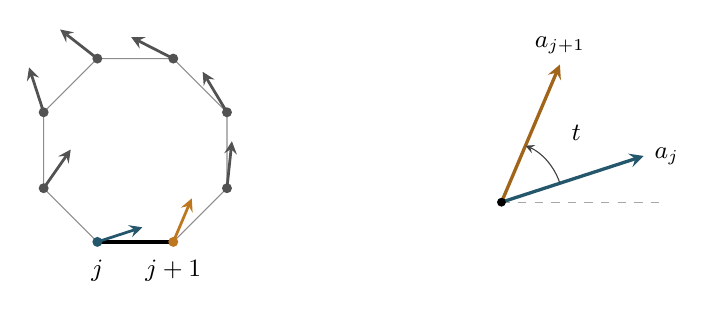
\begin{tikzpicture}[font=\small,>=stealth]
  \foreach \k in {0,...,7}
    \coordinate (s\k) at ({-112.5+45*\k}:1.26);
  \draw[black!45] (s0)--(s1)--(s2)--(s3)--(s4)--(s5)--(s6)--(s7)--cycle;
  \draw[black,line width=1.2pt] (s0)--(s1);
  \foreach \k/\angle/\tone in {0/18/glowblue,1/67/glowgold,2/84/black!68,
      3/121/black!68,4/153/black!68,5/142/black!68,6/108/black!68,7/55/black!68}{
    \draw[->,\tone,line width=1pt] (s\k)--++(\angle:.6);
    \fill[\tone] (s\k) circle[radius=1.8pt];
  }
  \node[below=3pt] at (s0) {$j$};
  \node[below=3pt] at (s1) {$j+1$};
  \begin{scope}[shift={(4.65,-.66)}]
    \draw[black!35,dashed] (0,0)--(2.1,0);
    \draw[->,glowblue,line width=1.2pt] (0,0)--(18:1.9)
      node[right,text=black] {$a_j$};
    \draw[->,glowgold!85!black,line width=1.2pt] (0,0)--(67:1.9)
      node[above,text=black] {$a_{j+1}$};
    \draw[->,black!75] (18:.78) arc[start angle=18,end angle=67,radius=.78];
    \node[fill=white,inner sep=1pt] at (43:1.30) {$t$};
    \fill (0,0) circle[radius=1.6pt];
  \end{scope}
\end{tikzpicture}
\caption{One spin configuration on the cycle. Translating the arrows at
$j$ and $j+1$ to a common origin makes their angular difference
$t=\theta_{j+1}-\theta_j$ visible.}\label{fig:spins}
\end{figure}

In the classical nearest-neighbor $XY$ model, the energy of 1 bond is
$1-\cos(\theta_{j+1}-\theta_j)$. At inverse temperature $\kappa>0$ a
configuration of energy $E$ receives weight proportional to $e^{-\kappa E}$.
Large $\kappa$ favors alignment. For a small angular difference $t$ the bond
energy is $t^2/2+O(t^4)$.

Villain \cite{villain} wanted to understand how the correlations between
distant spins change with temperature in a 2-dimensional planar magnet.
In particular, how can a phase transition occur even though there is no
spontaneous magnetization? A quadratic energy makes small angular
fluctuations easy to calculate, but assigns different energies to $t$ and
$t+2\pi$, which describe the same bond. Villain restored this periodicity by
summing the Gaussian weights of all real lifts $t+2\pi h$, $h\in\mathbb Z$.
In 2 dimensions, vortex pairs play a central role in the
Kosterlitz--Thouless description \cite{kth}. Fr\"ohlich and Spencer
\cite{fsp} proved the transition for the planar rotator and Villain models.
Here we use Villain's bond weight on a single cycle.
Let $dm(t)=dt/(2\pi)$ be uniform probability measure on the circle. Use
the parameter $l=2\kappa$, which is the stiffness of the bonds. The normalized bond density relative to $dm$
is
\[
 K_l(t)=\sqrt{\pi l}\sum_{h\in\mathbb Z}
           \exp\!\left[-\frac{l}{4}\,(t+2\pi h)^2\right]
       =\sum_{n\in\mathbb Z}e^{-n^2/l}e^{int}
\]
For the second equality integrate the first expression against $e^{-int}dm(t)$.
The intervals for the different lifts cover $\mathbb R$. The Gaussian Fourier
integral gives $e^{-n^2/l}$, and the absolutely convergent Fourier series
recovers the density. The coefficient at $n=0$ is 1. Equivalently, a
single angular increment has the law of a real Gaussian of variance
$2/l$ reduced modulo $2\pi$.

\begin{samepage}
\begin{defn}
The periodic Villain measure on $N$ spins has density
\[
 \frac1{P_N}\,\prod_{j=0}^{N-1}K_l(\theta_{j+1}-\theta_j)
       \prod_{j=0}^{N-1}dm(\theta_j),\qquad \theta_N=\theta_0
\]
Here $P_N$ is the normalizing constant, or partition function.
\end{defn}
\end{samepage}

The density is unchanged by a common rotation of all spins and by a cyclic
shift of the sites. Each individual spin is therefore uniform at every
temperature. It is their relative angles that record the interaction.
As $l\to0^+$, the Fourier series of $K_l$ tends uniformly to $1$, giving
independent uniform spins. On a line one may start at a uniform spin and
take independent wrapped Gaussian increments. The cycle requires their
sum to close modulo $2\pi$. Equivalently it is the Markov chain with this
transition density, conditioned to return to its initial angle, with a
uniform initial angle. The product density above makes this bridge
interpretation precise even though an exact return has probability 0.

\medskip

\noindent\textbf{Why $l$ is a length.} 
On the infinite line the product $a_r\bar a_0$ is the exponential of a
sum of $r$ independent increments for $r\geq0$. Each increment has first
Fourier coefficient $e^{-1/l}$. Consequently
\[
   E(a_r\bar a_0)=e^{-|r|/l},\qquad r\in\mathbb Z
\]
The correlation falls by the factor $e^{-1}$ over $l$ lattice spacings.
On a finite cycle there are 2 paths joining a pair of sites, and closing
the chain changes the answer. We compute that change next.

\medskip

\noindent\textbf{The transfer operator.} 
A single step of the chain averages a function $f$ of the next angle by
\[
   (Tf)(s)=\int K_l(t-s)f(t)\,dm(t)
\]
The functions $e_n(t)=e^{int}$ form the Fourier basis on the circle, and
$Te_n=e^{-n^2/l}e_n$. Integrating out successive sites on the cycle
composes the kernels. Closing the last bond integrates the diagonal of
$T^N$, so $P_N=Tr(T^N)=\sum_n e^{-Nn^2/l}$.
Multiplication by a spin sends $e_n$ to $e_{n+1}$, and multiplication by
its conjugate sends $e_n$ to $e_{n-1}$. This simple shift explains why
4 spin insertions can be computed explicitly.

Here is a convenient bond version of the same rule. Put an integer $h_j$
on each directed bond $j\to j+1$ and consider the product of its increment
raised to $h_j$. Expanding each factor of the density in Fourier series
and integrating each angle enforces equality of the total incoming and
outgoing index at that site. The total index on every bond is therefore
a single integer $n$. Using the evenness of the squared index gives
\[
 E\left[\prod_{j\in G}(a_{j+1}\bar a_j)^{h_j}\right]
   =\sum_{n\in\mathbb Z}
      \exp\!\biggl[-\sum_{j\in G}(n+h_j)^2/l\biggr]
      \,\Big/\,\sum_{n\in\mathbb Z}e^{-Nn^2/l}
\]
Indeed the Fourier index of the density on bond $j$ is $n-h_j$,
and one can change $n$ to $-n$ in the sum. Absolute convergence in
the Fourier series of $K_l$ justifies termwise integration. Adding an integer
constant to all $h_j$ leaves both sides unchanged, as the product of
all bond increments around the cycle is 1.

\begin{samepage}
\begin{prop}\label{prop:twopoint}
Let $C_N(r)=E(a_r\bar a_0)$. For $0\leq r\leq N$,
\[
 C_N(r)=
 \sum_{n\in\mathbb Z}e^{-[(N-r)n^2+r(n+1)^2]/l}
      \,\Big/\,\sum_{n\in\mathbb Z}e^{-Nn^2/l}
\]
In particular $C_N(0)=1$ and $C_N(r)=C_N(N-r)$ is real.
\end{prop}
\end{samepage}
\begin{proof}
Use $h_j=1$ on the first $r$ bonds and 0 elsewhere in
the bond expectation formula of Section~\ref{sec:villain}. The product on the left telescopes to $a_r\bar a_0$.
The change of variable $n\to-1-n$ interchanges the 2 arcs.
\end{proof}

For fixed $N$, $C_N(r)\to1$ as $l\to\infty$. To see this, complete
the square in the numerator, obtaining the factor
$e^{-r(1-r/N)/l}$ times $\sum_n e^{-N(n+r/N)^2/l}$.
After dividing both Gaussian sums by $\sqrt{l/N}$, they are Riemann
sums for the same integral. Thus $E(|a_r-a_0|^2)=2(1-C_N(r))\to0$.
The configuration at temperature 0 consists of 1 uniform spin repeated
around the cycle.

In higher dimensions, closed paths through a lattice permit configurations
of angular increments of a much richer kind. Dario and Wu \cite{dariowu}
prove that the truncated Villain 2-point function decays as $|x|^{2-d}$ on $\mathbb Z^d$ at sufficiently low temperature, for $d\geq3$. Here the cycle has a single closing
condition, which is accounted for by the 1 summation index in
the bond expectation formula of Section~\ref{sec:villain}.

\section{The 4-spin parallelogram identity}\label{sec:two}\label{sec:four}

Let $a,b$ be independent periodic Villain chains on $G$, with the same
parameter $l$. Our random variable and its perfectly aligned counterpart are
\[
  Z_N=\frac1N\,\sum_{jk\in G}w^{jk}\bar a_jb_k,\qquad
  U_0=\bar a_0 b_0
\]
The variable $U_0$ is a uniform phase for all $l$. If both chains are
constant then $Z_N=U_0$, since the sum of all entries of $F$ is $N$ by
Fourier orthogonality. The opposite endpoint, $l=0$, is the normalized
glow of Section~\ref{sec:glow}.

\begin{samepage}
\begin{prop}\label{prop:two}
The law of $Z_N$ is invariant under rotations of $\mathbb C$. At every $N$ and
$l$ we have $E(Z_N)=0$ and $E(|Z_N|^2)=1$.
\end{prop}
\end{samepage}
\begin{proof}
A common rotation of $b$ multiplies $Z_N$ by that phase and preserves the
law. For the 2nd moment let $B=E(bb^*)$. Its entries are
$B_{kl}=C_N(k-l)$ by stationarity. Changing variables from $k,l$ to
$k-l,l$ and applying Fourier orthogonality shows that $FBF^*$ is diagonal.
Hence, conditional on $a$,
\[
  E_b(|Z_N|^2)=\frac1{N^2}\,\langle FBF^*a,a\rangle
   =\frac1{N^2}\,Tr(FBF^*)=\frac1N\,Tr B=1
\]
The middle equality uses $|a_j|=1$. This proof needs only the stationarity
of the second chain and its independence from the first.
\end{proof}

\medskip

\noindent\textbf{An overlap with the aligned configuration.} 
There is a way to see the relevant length before considering the 4th
moment. The quantity $E(Z_N\bar U_0)$ measures how closely the glow
follows the particular phase selected by the spins at the origins. Since
both variables have 2nd moment 1, their mean square distance equals
$2-2Re\,E(Z_N\bar U_0)$.

\begin{samepage}
\begin{prop}\label{prop:overlap}
Suppose $l/\sqrt N\to c$ with $0<c<\infty$. Then $E(Z_N\bar U_0)$
converges to
\[
 L(c)=\int_{\mathbb R^2} e^{-\frac{|s|+|t|}{c}}\cos(2\pi st)\,ds\,dt
     =\frac2\pi\,\int_0^\infty
           \frac{e^{-\frac{v}{2\pi c^2}}}{1+v^2}\,dv
\]
This is strictly increasing in $c$, from 0 to 1.
\end{prop}
\end{samepage}
\begin{proof}
Independence gives the exact sum
\[
  E(Z_N\bar U_0)=\frac1N\,\sum_{jk\in G}C_N(j)C_N(k)w^{jk}
\]
We verify the Riemann-sum limit, including the effect of closing the
chain. For $0\le r\le N/2$, pull $e^{-r/l}$ out of the numerator
in Proposition~\ref{prop:twopoint}. The remaining terms are
$e^{-(Nn^2+2rn)/l}$. For $N/l\ge1$ they are bounded by
$e^{-(n^2-|n|)}$, which is summable over $n$. For $r=O(\sqrt N)$
every term with $n\ne0$ goes uniformly to 0 on each bounded rescaled
interval. The denominator tends to 1 as well. Thus
$C_N(r)/e^{-r/l}\to1$ there, and on the entire half-cycle
$0\le C_N(r)\le C e^{-r/l}$ for an absolute constant $C$.

Take centered representatives of the sites. With $s=j/\sqrt N$ and
$t=k/\sqrt N$ the Fourier phase becomes $2\pi st$ and the grid area is
$1/N$. On bounded rectangles the ordinary Riemann sums converge.
The exponential bounds give uniformly small tails outside large rectangles
by summing 2 geometric series. Symmetry cancels the imaginary part.
Finally, integrating in $t$ gives $2c/(1+(2\pi cs)^2)$. The substitution
$v=2\pi c|s|$ gives the last integral in the statement. Its positive
integrand increases strictly with $c$, with the stated limits by dominated
convergence.
\end{proof}

\medskip
\noindent\textbf{The parallelogram.}
For a site $x\in G$ let $d(x)=|x|_N$ be its distance from 0 on the
cycle. Thus $d(x)=\min(x,N-x)$ for $0\le x<N$. We first determine which
4-spin function is selected by the glow, and then evaluate it.

\begin{samepage}
\begin{lem}\label{lem:reduction}
Put $A(x,y)=E(a_0a_{x+y}\bar a_x\bar a_y)$. We have
\[
 E(|Z_N|^4)=\frac1{N^2}\,
   \sum_{xyuv\in G} A(x,y)\overline{A(u,v)}\,w^{-xv-yu}
\]
for the 2 independent stationary chains with the same law.
\end{lem}
\end{samepage}
\begin{proof}
In $Z_N^2\bar Z_N^2$ denote the 4 site indices of the first chain
by $j_1,j_2,j_3,j_4$, with the first 2 coming from $Z_N$. Similarly
write $k_1,k_2,k_3,k_4$ for the second chain. Their expectations factor.
The phase is
\[
 w^{j_1k_1+j_2k_2-j_3k_3-j_4k_4}
\]
Translating all $j$ indices by 1 site leaves the spin expectation
unchanged and multiplies the phase by $w^{k_1+k_2-k_3-k_4}$. Averaging
over this translation forces $k_1+k_2=k_3+k_4$ in $G$. Translating all
$k$ indices similarly forces $j_1+j_2=j_3+j_4$. Thus the surviving $j$
quadruples are exactly
\[
   (p+x,\ p+y,\ p,\ p+x+y)
\]
and the $k$ quadruples are $(q+u,q+v,q,q+u+v)$. All parameters are in $G$
and the parametrization is unique. The exponent reduces to $-xv-yu$.
The $N^2$ choices of the 2 base points $p,q$ cancel 2 of the 4
factors of $N$ in the normalization. This proves the formula of Lemma~\ref{lem:reduction}.
\end{proof}

\begin{samepage}
\begin{thm}\label{thm:para}
For the periodic Villain chain, we have
\[
  A(x,y)=\exp\!\left[-\frac2l\,\min(d(x),d(y))\right]
\]
for all $x,y\in G$, $N\ge1$, and $l>0$.
\end{thm}
\end{samepage}
\begin{proof}
Interchanging $x,y$ preserves the observable. Changing $x$ to $-x$ and
translating the 4 sites by $x$ conjugates it. All such expectations
are real by the symmetry $\theta\to-\theta$. The same applies to
$y$. We may therefore take centered representatives with
$0\le x\le y\le N/2$. In this order $x+y\le N$. The product is
\[
   (\bar a_x a_0)(a_{x+y}\bar a_y)
\]
It uses the first $x$ bonds with exponent $-1$ and the $x$ bonds starting
at $y$ with exponent $+1$. The arcs have disjoint bond interiors even when
their endpoints meet. All other bond exponents vanish. The exponent sum in
the bond expectation formula of Section~\ref{sec:villain} is thus
\[
   x(n-1)^2+x(n+1)^2+(N-2x)n^2=Nn^2+2x
\]
The term $2x$ is independent of $n$, so the quotient of the 2 sums is
$e^{-2x/l}$. The formula also gives 1 when either side of the
parallelogram is 0, as it must.
\end{proof}

Figure~\ref{fig:arcs} shows these bond exponents on the cycle cut at 0.

\begin{figure}[htb!]
\centering
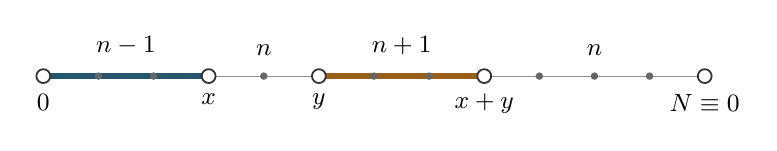
\begin{tikzpicture}[x=7.0mm,y=1cm,font=\small]
  \draw[black!45] (0,0)--(12,0);
  \draw[line width=2pt,glowblue] (0,0)--(3,0);
  \draw[line width=2pt,glowgold!80!black] (5,0)--(8,0);
  \foreach \i in {0,...,12} \fill[black!60] (\i,0) circle[radius=1.35pt];
  \foreach \i/\name in {0/0,3/x,5/y,8/{x+y},12/{N\equiv0}}
    {\draw[black!80,fill=white,line width=.65pt] (\i,0) circle[radius=2.5pt];
     \node[below=3pt] at (\i,0) {$\name$};}
  \node[above=4pt] at (1.5,0) {$n-1$};
  \node[above=4pt] at (4,0) {$n$};
  \node[above=4pt] at (6.5,0) {$n+1$};
  \node[above=4pt] at (10,0) {$n$};
\end{tikzpicture}
\caption{The 2 marked arcs have $x$ bonds each. One shifts the Fourier
index down by 1 and the other shifts it up by 1. The 2 ends of the
drawing represent the same site.}\label{fig:arcs}
\end{figure}

The cancellation is particular to the heat kernel. Its Fourier eigenvalues
have a quadratic logarithm, whose second difference is constant. This is
why the closing condition, so visible in the 2-spin function, disappears
from the answer for these 4 spins.

\section{The 4th-moment crossover function}\label{sec:cross}\label{sec:limits}

\medskip

\noindent\textbf{An exact formula at finite size.} 
For integers $r,s\ge0$ define $I_r=\{j\in G:d(j)\le r\}$ and
\[
 D_N(r,s)=\frac1N\,\sum_{j\in I_r,\ k\in I_s} w^{jk}
\]
This number is real by the symmetry of either interval. An interval
of radius at least $\lfloor N/2\rfloor$ is understood as the whole cycle.
Let $U,V$ be independent exponential random variables of mean 1, so
$P(U\ge t)=e^{-t}$ for $t\ge0$.

\begin{samepage}
\begin{thm}\label{thm:finite}
Put $R=\lfloor l U/2\rfloor$ and $S=\lfloor l V/2\rfloor$. We have
\[
        E(|Z_N|^4)=1+E\big[(1-D_N(R,S))^2\big]
\]
where $U,V$ are independent exponential variables of mean 1.
\end{thm}
\end{samepage}
\begin{proof}
Write $h_r(j)=1$ when $d(j)>r$, and $h_r(j)=0$ otherwise. By Theorem~\ref{thm:para},
\[
  A(x,y)=1-E[h_R(x)h_R(y)]
\]
Indeed, the product of the 2 indicators is 1 exactly when the
integer $\min(d(x),d(y))$ exceeds $R$. Use independent radii for the 2
copies of $A$ in the formula of Lemma~\ref{lem:reduction}. The constant times constant term is
1. Both mixed terms vanish because summing over the other 2 variables
forces the arguments of $h_r$ to be 0, and $h_r(0)=0$. The remaining
sum factors into the square of
\[
  \frac1N\,\sum_{jk}h_R(j)h_S(k)w^{-jk}
\]
Expand each $h$ as 1 minus an interval indicator. By Fourier orthogonality
and reality, the 4 resulting terms are $1$, $-1$, $-1$ and $D_N(R,S)$.
Squaring gives the formula.
\end{proof}

As a check, at $l\to0^+$ both radii tend to 0 almost surely and
$D_N(0,0)=1/N$. This gives exactly $2-2/N+1/N^2$, the independent-phase
answer. At fixed $N$ and $l\to\infty$, both intervals eventually fill
the cycle, and one recovers the 4th moment 1.

\begin{samepage}
\begin{thm}\label{thm:critical}
If $l/\sqrt N\to c$ with $0<c<\infty$, then $E(|Z_N|^4)\to M(c)$, where
\[
 M(c)=1+E\left[
   \left(1-\frac2\pi\, Si\!\left(\frac{\pi c^2}2\,UV\right)\right)^2
 \right],\qquad
 Si(t)=\int_0^t\frac{\sin v}{v}\,dv
\]
with $U,V$ independent exponential variables of mean 1.
\end{thm}
\end{samepage}
\begin{proof}
Fix $U,V>0$. In the variables $x=j/\sqrt N$, $y=k/\sqrt N$, the 2
intervals converge after rescaling to $[-a,a]$ and $[-b,b]$, where
$a=cU/2$ and $b=cV/2$. They do not wrap around the cycle for all
sufficiently large $N$. The grid area is $1/N$, so
\[
 D_N(R,S)\to
 \int_{-a}^a\int_{-b}^b e^{2\pi ixy}\,dy\,dx
 =\frac2\pi\,\int_0^{2\pi ab}\frac{\sin v}{v}\,dv
\]
For the last equality the inner integral is $\sin(2\pi bx)/(\pi x)$
with its continuous value at $x=0$. Since $l/\sqrt N$ is bounded,
\[
 |D_N(R,S)|\le\frac{(2R+1)(2S+1)}{N}\le C(1+U)(1+V)
\]
The square of this bound is integrable for exponential $U,V$. Dominated
convergence in Theorem~\ref{thm:finite} proves the result.
\end{proof}

\medskip

\noindent\textbf{Strict monotonicity.} 
The function $Si$ oscillates about its limit $\pi/2$.
It is the averaging over the radii that enforces the ordering in $c$.

\begin{samepage}
\begin{prop}\label{prop:monotone}
$M$ is continuous and strictly decreasing on $(0,\infty)$, with
$M(0+)=2$ and $M(+\infty)=1$.
\end{prop}
\end{samepage}
\begin{proof}
Put $q(t)=1-(2/\pi)Si(t)$. The Dirichlet integral is
$\int_0^\infty \sin v\,dv/v=\pi/2$. For completeness, inserting a
factor $e^{-\epsilon v}$ and differentiating the damped integral of
$\sin(bv)/v$ in $b$ gives $\epsilon/(\epsilon^2+b^2)$; integration from
$0$ to $1$ gives $\arctan(1/\epsilon)$. Integration by parts bounds the
damped and undamped tails beyond $A$ by $2/A$, uniformly in $\epsilon\ge0$,
so one may let $\epsilon$ go to 0. It follows that $q$ is bounded,
$q(0)=1$, $q(\infty)=0$, and for $t>0$
\[
  q(t)=\frac2\pi\,\int_1^\infty\frac{\sin(tu)}u\,du
\]

First average over just 1 exponential. For $s>0$, differentiation gives
\[
 \frac{d}{ds}\,E[q(sU)^2]=-\frac4{\pi s}\,E[q(sU)\sin(sU)]
\]
The differentiated integrand is bounded locally uniformly in $s>0$.
For any $u>0$, the product-to-sum identity and the exponential density give
\[
 E[\sin(sU)\sin(suU)]=\frac12\,
 \left(\frac1{1+s^2(u-1)^2}-\frac1{1+s^2(u+1)^2}\right)>0
\]
Insert the representation of $q$ truncated at $u=B$. Fubini's theorem
applies on $[1,B]$. The truncated integrals are bounded uniformly in
$B,t$ by boundedness of $Si$, so they converge also inside the expectation.
The resulting integral of the displayed positive expression against $du/u$
is strictly positive. Thus the average over 1 exponential variable is strictly
decreasing. Set $s=\pi c^2 V/2$ and average over $V>0$ to obtain strict
decrease of $M$. Continuity and the 2 endpoints follow by bounded
convergence applied to $q^2$.
\end{proof}

Figure~\ref{fig:crossover} shows how $M(c)$ leaves the Gaussian value and
approaches the circle value. Direct quadrature gives the following rounded values.
One can integrate in the single variable $t=UV$, whose density is
$\int_0^\infty e^{-u-t/u}\,du/u$ by a change of variables. The program
\texttt{crossover.py} does this, in the variable $z=\sqrt{UV}$, and also
produces the 65 points of Figure~\ref{fig:crossover}.
\begin{center}
\begin{tabular}{c@{\qquad}ccccc}
\toprule
$c$ & $\frac14$ & $\frac12$ & $1$ & $2$ & $4$\\
\midrule
$M(c)$ & $1.89106$ & $1.69450$ & $1.41935$ & $1.19882$ & $1.07900$\\
\bottomrule
\end{tabular}
\end{center}

\begin{figure}[H]
\centering
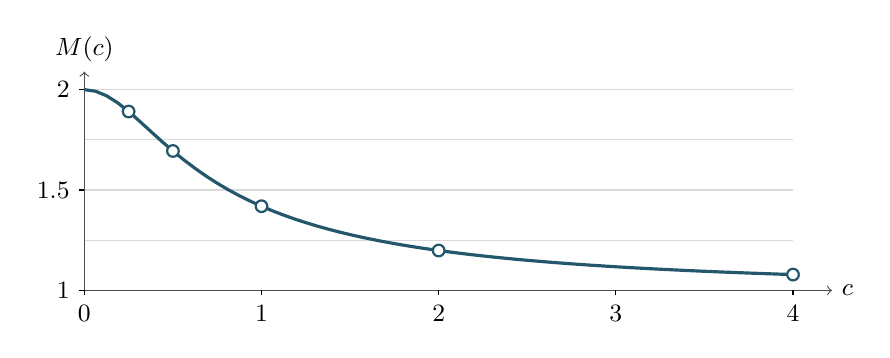
\begin{tikzpicture}[x=2.25cm,y=2.55cm,font=\small]
  \foreach \y in {1.25,1.5,1.75,2}
    \draw[black!15] (0,\y)--(4,\y);
  \draw[->,black!70] (0,1)--(4.22,1) node[right,text=black] {$c$};
  \draw[->,black!70] (0,1)--(0,2.09) node[above,text=black] {$M(c)$};
  \foreach \x in {0,1,2,3,4}
    \draw (\x,1)--++(0,-.024) node[below] {$\x$};
  \foreach \y in {1,1.5,2}
    \draw (0,\y)--++(-.028,0) node[left] {$\y$};
  \draw[glowblue,line width=1.15pt,line join=round] plot coordinates {
    (0.0000,2.000000) (0.0625,1.992249) (0.1250,1.969755) (0.1875,1.934834) (0.2500,1.891063)
    (0.3125,1.842338) (0.3750,1.791941) (0.4375,1.742189) (0.5000,1.694503) (0.5625,1.649641)
    (0.6250,1.607928) (0.6875,1.569415) (0.7500,1.534005) (0.8125,1.501514) (0.8750,1.471727)
    (0.9375,1.444414) (1.0000,1.419351) (1.0625,1.396328) (1.1250,1.375149) (1.1875,1.355635)
    (1.2500,1.337626) (1.3125,1.320978) (1.3750,1.305560) (1.4375,1.291258) (1.5000,1.277968)
    (1.5625,1.265598) (1.6250,1.254066) (1.6875,1.243297) (1.7500,1.233226) (1.8125,1.223793)
    (1.8750,1.214945) (1.9375,1.206635) (2.0000,1.198820) (2.0625,1.191460) (2.1250,1.184520)
    (2.1875,1.177968) (2.2500,1.171776) (2.3125,1.165917) (2.3750,1.160368) (2.4375,1.155106)
    (2.5000,1.150112) (2.5625,1.145367) (2.6250,1.140855) (2.6875,1.136560) (2.7500,1.132469)
    (2.8125,1.128568) (2.8750,1.124846) (2.9375,1.121291) (3.0000,1.117894) (3.0625,1.114645)
    (3.1250,1.111535) (3.1875,1.108557) (3.2500,1.105702) (3.3125,1.102965) (3.3750,1.100338)
    (3.4375,1.097815) (3.5000,1.095391) (3.5625,1.093061) (3.6250,1.090820) (3.6875,1.088663)
    (3.7500,1.086586) (3.8125,1.084584) (3.8750,1.082655) (3.9375,1.080795) (4.0000,1.079000)};
  \foreach \p in {{(0.25,1.891063)},{(0.50,1.694503)},{(1.00,1.419351)},{(2.00,1.198820)},{(4.00,1.079000)}}
    \filldraw[draw=glowblue,fill=white,line width=.8pt] \p circle[radius=2.1pt];
\end{tikzpicture}
\caption{The limiting fourth moment at correlation length $l\sim c\sqrt N$.
Circles mark the 5 tabulated values.}\label{fig:crossover}
\end{figure}

\medskip
\noindent\textbf{Limits outside the crossover.}
We have taken $N\to\infty$ at a fixed positive value of $c$. To describe
a chain with $l/\sqrt N$ itself tending to 0 or infinity, we return
to the finite formula.

\begin{samepage}
\begin{thm}\label{thm:sides}
If $l/\sqrt N\to0$, then $E(|Z_N|^4)\to2$. If $l/\sqrt N\to\infty$,
then $E(|Z_N|^4)\to1$ and $Z_N$ converges in law to the uniform measure
on the unit circle.
\end{thm}
\end{samepage}
\begin{proof}
In the first regime, $(2R+1)(2S+1)/N\to0$ for each fixed $U,V$. The
integrable domination used in Theorem~\ref{thm:critical} gives the result.

In the second regime we need cancellation in the rectangular Fourier sum.
If either interval fills the cycle, $D_N(r,s)=1$. Otherwise put
$H=\lfloor N/2\rfloor$. Summing first in $k$ by a geometric progression
gives
\[
   1-D_N(r,s)=\frac1N\,\sum_{j\notin I_r}
     \frac{\sin\left(\frac{(2s+1)\pi j}{N}\right)}{\sin\left(\frac{\pi j}{N}\right)}
\]
Here the sum over all $j$, including the continuous value at $j=0$,
would give 1 after division by $N$. On the positive half-cycle
$r<j\le H$ the weights $1/\sin(\pi j/N)$ decrease, with first value
at most $C N/(r+1)$. The partial sums of the sines are at most
$1/\sin((2s+1)\pi/(2N))\le C N/(s+1)$ in absolute value, by summing
complex exponentials. Summation by parts and the factor $1/N$ give
\[
    |1-D_N(r,s)|\le\frac{C N}{(r+1)(s+1)}
\]
The negative half obeys the same bound; for even $N$ take the antipodal
site in only 1 half. This estimate also supplies a uniform bound when
$(r+1)(s+1)\ge N$. In the complementary case the elementary estimate
$|D_N(r,s)|\le (2r+1)(2s+1)/N\le4$ supplies it.

For fixed $U,V>0$, $(R+1)(S+1)/N\to\infty$. The last estimates give
$1-D_N(R,S)\to0$ with a uniform bound, including saturated intervals.
Theorem~\ref{thm:finite} now gives convergence of the 4th moment to 1.
Finally Proposition~\ref{prop:two} implies
\[
    E\big[(|Z_N|^2-1)^2\big]=E(|Z_N|^4)-1\to0
\]
Thus $|Z_N|\to1$ in probability. By rotation invariance, $Z_N$ has the
same law as $|Z_N|u$ with $u$ an independent uniform phase. This gives
the asserted convergence in law.
\end{proof}

The circle law already holds, for instance, when $l=N^{3/4}$. In that
example the correlation between 2 diametrically opposite spins still
tends to 0 by Proposition~\ref{prop:twopoint} and the bound in the
proof of Proposition~\ref{prop:overlap}. What aligns at this scale is the
modulus of the Fourier sum. The chain may still have many essentially
uncorrelated stretches around the cycle.

\begin{samepage}
\begin{question}\label{que:law}
When $l/\sqrt N\to c$ with $0<c<\infty$, does $Z_N$ converge in law?
If so, what is its radial distribution? On the hot side, does every
sequence with $l/\sqrt N\to0$ have the complex Gaussian limit?
\end{question}
\end{samepage}

The 2nd-moment bound gives tightness, and rotation invariance passes
to subsequential limits. The exact 4th moment gives a test for a
candidate crossover law once uniform integrability of $|Z_N|^4$ is known.
One way to proceed is to compute the 6th moment. The translation
argument of Lemma~\ref{lem:reduction} then selects 6 sites for which the
sum of the 3 positive indices equals the sum of the 3 negative
indices modulo $N$. The bond expectation formula of Section~\ref{sec:villain} still evaluates each spin
expectation. The ordering of 6 sites permits several arc patterns, and the
shorter-side formula of Theorem~\ref{thm:para} is what would need a successor.

\section{Villain glow of Hadamard matrices}\label{sec:general}

The construction of Section~\ref{sec:villain} makes sense for any complex Hadamard matrix $H$ of order $N$, once its rows and columns are labeled by the cycle $G$. Let $a,b$ be independent periodic Villain chains on $G$, with the same parameter $l$, and put
\[
 Z=\frac1N\,\langle Hb,a\rangle=\frac1N\,\sum_{jk\in G}H_{jk}\bar a_jb_k
\]
With the same-layer bond phases fixed, the law can depend on the representative and on the cyclic ordering within each layer. Independent global rotations of the chains and cyclic shifts and reflections of either set of labels preserve the law. Interchanging the identical chains and using conjugation symmetry also gives invariance under transposition.

The 2 extreme values of the stiffness are as follows. As $l\to0^+$ the spins become independent and uniform, and $Z$ is the normalized glow of $H$, from Section~\ref{sec:glow}. As $l\to\infty$ each chain becomes a single uniform phase, by the remark after Proposition~\ref{prop:twopoint}, and $Z$ tends in law to
\[
 \bar a_0b_0\cdot\frac1N\,\sum_{jk}H_{jk}
\]
Thus the cold limit is governed by the sum of the entries of $H$, that is, by its excess. For the Fourier matrix in the form $F=(w^{jk})$ this sum is $N$, which is the reason for the unit circle in Theorem~\ref{thm:sides}. By Cauchy--Schwarz the modulus of this sum is at most $N\sqrt N$, with equality precisely when all the row sums of $H$ are equal, which forces the column sums to be equal too, that is, when $H$ is bistochastic. Every complex Hadamard matrix has bistochastic representatives, by the Idel--Wolf theorem \cite{iwo}, so along an equivalence class the Villain parameter interpolates between an invariant, the glow, and a quantity which is maximized exactly at the bistochastic forms.

\medskip

\noindent\textbf{The 2nd moment.} Let $f_k=N^{-1/2}(w^{jk})_{j\in G}$ be the Fourier basis of $\mathbb C^N$, and let $c_0,\ldots,c_{N-1}$ be the eigenvalues of the correlation matrix $C=(C_N(j-k))_{j,k\in G}$, which is circulant. Since $C_N$ is even, we may write
\[
 c_k=\sum_{r\in G}C_N(r)w^{kr}
\]
These numbers are $\geq0$, since $C$ is a correlation matrix, and their mean is $C_N(0)=1$. For a matrix $H$ define a probability measure on $G\times G$ by
\[
 p_{kl}=\frac1{N^2}\,|\langle Hf_l,f_k\rangle|^2
\]
where $\langle x,y\rangle=\sum_jx_j\bar y_j$. The total mass is $N^{-2}\,Tr(HH^*)=1$. We call $p$ the Fourier mass of $H$.

\begin{samepage}
\begin{prop}\label{prop:general2}
For any complex Hadamard matrix $H$ of order $N$, we have
\[
 E(|Z|^2)=\frac1{N^2}\,Tr(CHCH^*)=\sum_{kl\in G}p_{kl}\,c_kc_l
\]
for every positive Villain parameter.
\end{prop}
\end{samepage}

\begin{proof}
Conditional on $a$, the computation in the proof of Proposition~\ref{prop:two} gives $E_b(|Z|^2)=N^{-2}\langle HCH^*a,a\rangle$. For a deterministic matrix $M$ we have $E(\langle Ma,a\rangle)=\sum_{jj'}E(\bar a_ja_{j'})M_{jj'}=Tr(CM)$, because $E(\bar a_ja_{j'})=C_N(j'-j)$ and $C$ is symmetric. This gives the first formula. For the second, write $C=\sum_kc_kf_kf_k^*$ and expand the trace.
\end{proof}

This formula explains Proposition~\ref{prop:two} from a different angle. For the Fourier matrix, $Ff_l=\sqrt N e_{-l}$ and $\langle Ff_l,f_k\rangle=w^{kl}$ has modulus 1 for all $k,l$, so the Fourier mass is uniform, and the 2nd moment is the square of the mean of the $c_k$, which is 1. For other matrices the 2nd moment may vary with $l$, and its cold limit is $p_{00}N^2=N^{-2}|\sum_{jk}H_{jk}|^2$, since $c_0\to N$ and $c_k\to0$ for $k\neq0$.

\begin{samepage}
\begin{prop}\label{prop:bist2}
If $H$ is bistochastic, then $E(|Z|^2)\geq c_0^2/N$. In particular, we have
\[
 \liminf_{N\to\infty}\ E(|Z|^2)\geq4c^2
\]
whenever $l/\sqrt N\to c$ with $0<c<\infty$.
\end{prop}
\end{samepage}

\begin{proof}
All the terms in Proposition~\ref{prop:general2} are $\geq0$. For a bistochastic matrix, $Hf_0=\lambda f_0$ with $|\lambda|=\sqrt N$, so $p_{00}=N/N^2=1/N$, which gives the first assertion. For the second, the bounds in the proof of Proposition~\ref{prop:overlap} show that $C_N(r)/e^{-r/l}\to1$ uniformly for $r=O(\sqrt N)$, and Riemann sums give $c_0/l\to\int_{\mathbb R}e^{-|s|}ds=2$.
\end{proof}

For $c>1/2$ this lower bound forces the 2nd moment of a bistochastic representative above its independent-phase value 1 in the limit. For $c\le1/2$ the bound alone does not decide its departure from 1. Alignment across the full cycle occurs on the larger scale $l\gg N$, and at fixed $N$ the aligned limit gives $E(|Z|^2)\to N$. The following values, at $N=16$, are given by Proposition~\ref{prop:general2}, and agree with exact sampling of the chains, with $10^5$ samples, to within the sampling error. The sampling uses the winding decomposition of the periodic chain: a winding number $n$ with weight proportional to $e^{-\pi^2n^2l/N}$, followed by a Gaussian bridge with increments of variance $2/l$ and total $2\pi n$. Both are done by the program \texttt{villaincheck.py}. Here $W$ is the Walsh matrix in its natural order, and $B$ is a bistochastic form of a real Hadamard matrix of order 16, with row sums 4.

\medskip

\begin{center}
\begin{tabular}{|c|c|c|c|c|c|c|}
\hline
$l$ & $0.5$ & $2$ & $8$ & $32$ & $128$ & $1024$\\
\hline
$F$ & $1$ & $1$ & $1$ & $1$ & $1$ & $1$\\
$W$ & $1.0045$ & $1.0657$ & $1.0174$ & $1.0015$ & $1.0001$ & $1.0000$\\
$B$ & $1.0046$ & $1.5769$ & $8.2924$ & $13.578$ & $15.351$ & $15.917$\\
\hline
\end{tabular}
\end{center}

\medskip

For the Walsh matrix the sum of the entries is $N$, so its 2nd moment returns to 1 at both ends, with a bump in between, coming from its Fourier mass, which is not uniform.

\medskip

\noindent\textbf{Group matrices and Cayley graphs.} The exact results of Sections~\ref{sec:two}--\ref{sec:cross} rest on a matching of symmetries: the Fourier matrix of $G=\mathbb Z_N$, and a spin model on the cycle, which is the Cayley graph of $\mathbb Z_N$ with generator 1. This matching extends. Let $G$ be a finite abelian group, let $F_G=(\chi(x))_{\chi\in\widehat G,x\in G}$ be its Fourier matrix, and let $a,b$ be independent phase fields on $\widehat G$ and $G$, indexing the rows and the columns, whose laws are invariant under translations. Fourier orthogonality gives $E(|Z|^2)=1$ by Proposition~\ref{prop:two}. For $\xi,\eta\in\widehat G$ and $u,v\in G$, denote the two parallelogram expectations of Lemma~\ref{lem:reduction} by $A_a(\xi,\eta)$ and $A_b(u,v)$ respectively, using additive notation in both groups. Averaging over translations in each layer gives
\[
 E(|Z|^4)=\frac1{|G|^2}\sum_{\xi,\eta\in\widehat G}\sum_{u,v\in G}
 A_a(\xi,\eta)\overline{A_b(u,v)\,\xi(v)\eta(u)}
\]
This is the same parallelogram selection rule, with the characters of $G$ providing the phase. The natural choice is the Villain model on a Cayley graph of $G$.

For $G=\mathbb Z_2^n$, with $N=2^n$, the Fourier matrix is the Walsh matrix $W_N$. Take the standard coordinate generators, and join two vertices when they differ in one coordinate. This is the hypercube. Like the cycle it admits a path through all vertices returning to its starting point. Its extra edges impose a closing constraint on every square face. Its diameter is only $n=\log_2N$. Figure~\ref{fig:cayley} illustrates the difference at $N=8$.

\begin{figure}[H]
\centering
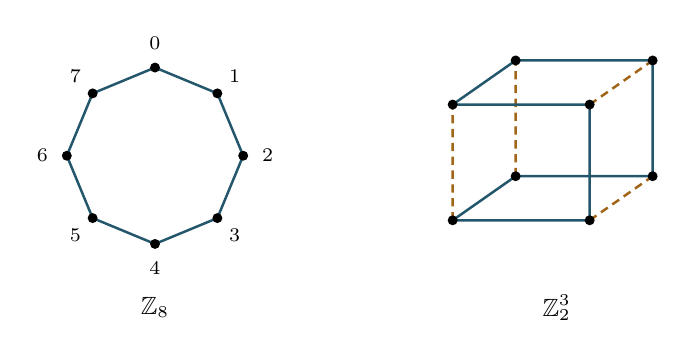
\begin{tikzpicture}[font=\small]
  \foreach \i in {0,...,7} \coordinate (c\i) at ({90-45*\i}:1.12);
  \draw[glowblue,line width=.9pt] (c0)--(c1)--(c2)--(c3)--(c4)--(c5)--(c6)--(c7)--cycle;
  \foreach \i in {0,...,7}{
    \fill (c\i) circle[radius=1.8pt];
    \node at ({90-45*\i}:1.43) {\scriptsize $\i$};
  }
  \node at (0,-1.93) {$\mathbb Z_8$};
  \begin{scope}[shift={(5.1,0)}]
    % Each coordinate flip gives one cube edge; blue is a Hamiltonian cycle.
    \foreach \v/\x/\y in {a/-1.32/-.82,b/.42/-.82,c/.42/.65,d/-1.32/.65,
                            e/-.52/-.26,f/1.22/-.26,g/1.22/1.21,h/-.52/1.21}
      \coordinate (\v) at (\x,\y);
    \draw[glowgold!85!black,densely dashed,line width=.9pt]
      (a)--(d) (b)--(f) (c)--(g) (e)--(h);
    \draw[glowblue,line width=.9pt]
      (a)--(b)--(c)--(d)--(h)--(g)--(f)--(e)--cycle;
    \foreach \v in {a,b,c,d,e,f,g,h} \fill (\v) circle[radius=1.8pt];
    \node at (0,-1.93) {$\mathbb Z_2^3$};
  \end{scope}
\end{tikzpicture}
\caption{Villain bonds on 8 sites. The solid loop visits every site
once in both graphs. 4 further bonds (dashed) close the square faces
of the cube.}\label{fig:cayley}
\end{figure}

The cube may be viewed as a lattice of side 2 in dimension $n$. The Villain 2-point function on $\mathbb Z^d$, $d\ge3$, is studied in \cite{dariowu}. Josephson arrays in large dimension are considered in \cite{par}, and the fully frustrated hypercube in \cite{mp3}. For the Walsh glow there are two different limits to consider. As $n$ grows, at what stiffness does its 4th moment leave the independent-phase value $2-2/N+1/N^2$? It would be interesting to obtain a crossover function as on the cycle, and to compare higher moments with the Walsh polynomials of Sections~\ref{sec:moments}--\ref{sec:walsh}. Here we can answer the question at the aligned end, by first keeping the cube fixed and increasing the stiffness.

Put one bond with the density $K_l$ of Section~\ref{sec:villain} on each undirected edge. For $n=1$ there is a single bond, and the only parallelogram expectation different from 1 is
\[
 A(1,1)=E(a_0^2\bar a_1^2)=e^{-4/l}
\]
by the 2nd Fourier coefficient of $K_l$. In the Walsh formula for $E(|Z|^4)$ the terms linear in $A-1$ vanish by character orthogonality, leaving
\[
 E(|Z|^4)=1+\tfrac14(1-e^{-4/l})^2
\]
Thus the first correction to the circle value is $4/l^2$. The cancellation of the linear term persists in every dimension. The coefficient depends on the spectrum of the cube, and Figure~\ref{fig:cube-coeff} shows its dependence on $n$ after rescaling. The program \texttt{hypercube.py} computes the plotted coefficients by grouping pairs of supports by their sizes and the size of their intersection.

\begin{figure}[H]
\centering
\begin{tikzpicture}[x=16mm,y=1.05mm,font=\small]
  \foreach \y in {16,32,48}{
    \draw[black!14] (0,\y)--(7,\y);
    \node[left] at (0,\y) {$\y$};}
  \draw[->,black!70] (0,0)--(7.35,0) node[right] {$n$};
  \draw[->,black!70] (0,0)--(0,51) node[above] {$n^2c_n$};
  \foreach \pos/\val in {0/1,1/2,2/4,3/8,4/16,5/32,6/64,7/128}{
    \draw[black!60] (\pos,0)--(\pos,-1) node[below] {$\val$};}
  \draw[glowgold!85!black,thick,dashed] (0,32)--(7.15,32);
  \draw[glowblue,thick] plot[mark=*,mark size=1.45pt] coordinates {
    (0.000000,4.000000) (1.000000,16.000000) (1.584963,28.375000) (2.000000,37.111111)
    (2.321928,41.953559) (2.584963,43.957188) (2.807355,44.248572) (3.000000,43.655210)
    (3.169925,42.690835) (3.321928,41.638835) (3.584963,39.743597) (3.807355,38.309934)
    (4.000000,37.273365) (4.321928,35.947704) (4.584963,35.156009) (5.000000,34.257390)
    (5.584963,33.441131) (6.000000,33.058992) (6.584963,32.692205) (7.000000,32.514184)
  };
\end{tikzpicture}
\caption{The fixed-cube coefficient $n^2c_n$ at selected integer dimensions on a logarithmic horizontal scale. The points first rise above the limiting value 32 (dashed), then approach it from above over the dimensions shown.}\label{fig:cube-coeff}
\end{figure}

\begin{samepage}
\begin{thm}\label{thm:hypercube}
Let $a,b$ be independent Villain phase fields on the hypercube $G=\mathbb Z_2^n$, with one bond of stiffness $l$ on each undirected edge. Put $N=2^n$, let $W_N=((-1)^{x\cdot y})_{x,y\in G}$ and set $Z=\langle W_N b,a\rangle/N$. At each fixed $n\ge1$, as $l\to\infty$ we have
\[
 E(|Z|^4)=1+\frac{c_n}{l^2}+O_n(l^{-3}),\qquad
 c_n=\frac{16}{N^2}\sum_{\substack{s,t\in G\\s\cdot t=1}}\frac{1}{|s|\,|t|}
\]
where the dot product is taken modulo 2 and $|s|$ counts the nonzero coordinates of $s$. The coefficients satisfy $n^2c_n\to32$ as $n\to\infty$.
\end{thm}
\end{samepage}

\begin{proof}
First consider one phase field. By a common rotation we can pin its angle at the origin to zero. The Villain bond weight is a periodized Gaussian with exponent $-l u^2/4$. In a sufficiently small box of pinned angles about zero, all edge differences lie in $(-\pi/2,\pi/2)$. The noncentral lifts of each difference contribute a relative error $O(e^{-c l})$. Outside the box, the sum of the squared distances of the differences to $2\pi\mathbb Z$ has a strictly positive minimum: the cube is connected and all differences vanish modulo $2\pi$ only at the pinned aligned configuration. Hence the exterior has exponentially small mass after normalization. Indeed, the central Gaussian integral in the box, after removing the common bond prefactors, has order $l^{-(N-1)/2}$. The same estimate permits extending that Gaussian integral to all of $\mathbb R^{N-1}$. The exponential constants here can depend on $n$.

Write $L$ for the graph Laplacian, and $L^+$ for its inverse on the space perpendicular to constants, extended by zero on constants. The central Gaussian density is proportional to $\exp(-l\sum_{x\sim y}(\theta_x-\theta_y)^2/4)$, the sum using each edge once. Thus a neutral charge vector $q$, meaning $\sum_x q_x=0$, has Gaussian characteristic function $\exp(-q^tL^+q/l)$. One can subtract the average of the pinned angles to work on the space perpendicular to constants: this linear change has constant Jacobian and preserves both the energy and $q^t\theta$.

Take $q=\delta_0+\delta_{x+y}-\delta_x-\delta_y$, so that the characteristic function is the parallelogram expectation. The normalized characters $N^{-1/2}\chi_s(z)$, with $\chi_s(z)=(-1)^{s\cdot z}$, diagonalize $L$ with eigenvalues $2|s|$. Indeed, flipping a coordinate changes the sign of $\chi_s$ just when that coordinate belongs to the support of $s$. The unnormalized Fourier coefficient of $q$ is $(1-\chi_s(x))(1-\chi_s(y))$. Writing $h_s(x)=(1-\chi_s(x))/2$, we obtain
\[
 D(x,y)=q^tL^+q=\frac8N\sum_{s\ne0}\frac{h_s(x)h_s(y)}{|s|},
 \qquad A(x,y)=1-D(x,y)/l+O_n(l^{-2})
\]
uniformly over the finite cube. In fact the preceding Gaussian computation gives $A(x,y)=e^{-D(x,y)/l}+O_n(e^{-c_n' l})$ for some $c_n'>0$.

The fourth moment formula above uses the sign $\chi_x(v)\chi_y(u)$. Put $B=A-1$. The constant term is 1, and each linear term in $B$ vanishes, because summing over the other two variables selects $B(0,0)=0$. Both fields have the same law, and $A$ is real by conjugation symmetry. Consequently
\[
 E(|Z|^4)-1=\frac1{N^2}\sum_{x,y,u,v\in G}
                  B(x,y)B(u,v)\chi_x(v)\chi_y(u)
\]
The coefficient of $l^{-2}$ is the same expression with both factors $B$ replaced by $D$, with remainder $O_n(l^{-3})$. For each $s,t$ in the expansion of $D$ the sum factors into the square of
\[
 \frac1N\sum_{x,v\in G}h_s(x)h_t(v)\chi_x(v)=\frac{\chi_s(t)-1}{4}
\]
by Walsh orthogonality. Its square is $1/4$ for $s\cdot t=1$ and zero otherwise. Multiplication by $(8/N)^2$ gives the stated formula for $c_n$.

Finally take $s,t$ independently uniform on $G$. Given $s\ne0$, exactly half the choices of $t$ have $s\cdot t=1$, so this event has probability $(1-2^{-n})/2$. Both weights are binomial with parameters $n,1/2$. The probability that either weight lies outside $[n/4,3n/4]$ is exponentially small in $n$, and on $s\cdot t=1$ we always have $n^2/(|s|\,|t|)\le n^2$. On the central event the ratio is bounded by 16 and tends to 4 in probability. Therefore its expectation restricted to odd dot product, with zero assigned to the other pairs, tends to $4/2=2$. The factor 16 in $c_n$ gives the limit 32.
\end{proof}

\begin{thebibliography}{99}
\small\setlength{\itemsep}{1pt}\setlength{\parsep}{0pt}
\phantomsection\addcontentsline{toc}{section}{References}
\bibitem{abf}
Astra, Banica and Fable, Karlsson matrices and the kagome lattice, {\hypersetup{allcolors=black}\href{https://zenodo.org/records/24221202}{zenodo.org/records/24221202}} (2026).
\bibitem{ba0}
T. Banica, First order deformations of the Fourier matrix, \emph{J. Math. Phys.} \textbf{55} (2014), 012201.
\bibitem{banica}
T. Banica, The glow of Fourier matrices: universality and fluctuations,
\emph{Oper. Matrices} \textbf{9} (2015), 457--474.
\bibitem{bes}
M.R. Best, The excess of a Hadamard matrix, \emph{Indag. Math.} \textbf{39} (1977), 357--361.
\bibitem{bep}
P. Biran, M. Entov and L. Polterovich, Calabi quasimorphisms for the symplectic ball, \emph{Commun. Contemp. Math.} \textbf{6} (2004), 793--802.
\bibitem{bjo}
G. Bj\"orck, Functions of modulus 1 on $\mathbb Z_n$ whose Fourier transforms have constant modulus, and cyclic $n$-roots, in ``Recent advances in Fourier analysis and its applications'', Kluwer (1990), 131--140.
\bibitem{cfi}
P. Chandra, M.V. Feigel'man and L.B. Ioffe, Glass formation in a periodic long-range Josephson array, \emph{Phys. Rev. Lett.} \textbf{76} (1996), 4805--4808.
\bibitem{cfk}
P. Chandra, M.V. Feigel'man, L.B. Ioffe and D.M. Kagan, History dependence and aging in a periodic long-range Josephson array, \emph{Phys. Rev. B} \textbf{56} (1997), 11553.
\bibitem{cis}
P. Chandra, L.B. Ioffe and D. Sherrington, Possible glassiness in a periodic long-range Josephson array, \emph{Phys. Rev. Lett.} \textbf{75} (1995), 713--716.
\bibitem{chu}
D.C. Chu, Polyphase codes with good periodic correlation properties, \emph{IEEE Trans. Inform. Theory} \textbf{18} (1972), 531--532.
\bibitem{dariowu}
P. Dario and W. Wu, Massless phases for the Villain model in $d\geq3$,
\emph{Ast\'erisque} \textbf{447} (2024), 221 pp.
\bibitem{dvb}
A. De Vos and S. De Baerdemacker, Scaling a unitary matrix, \emph{Open Syst. Inf. Dyn.} \textbf{21} (2014), 1450013.
\bibitem{dez}
A. Dembo and O. Zeitouni, \emph{Large deviations techniques and applications}, 2nd ed., Springer (1998).
\bibitem{dita}
P. Di\c t\u a, Some results on the parametrization of complex Hadamard matrices, \emph{J. Phys. A} \textbf{37} (2004), 5355--5374.
\bibitem{fko}
N. Farmakis and S. Kounias, The excess of Hadamard matrices and optimal designs, \emph{Discrete Math.} \textbf{67} (1987), 165--176.
\bibitem{fsl}
P.C. Fishburn and N.J.A. Sloane, The solution to Berlekamp's switching game, \emph{Discrete Math.} \textbf{74} (1989), 263--290.
\bibitem{fza}
R.L. Frank, S.A. Zadoff and R.C. Heimiller, Phase shift pulse codes with good periodic correlation properties, \emph{IRE Trans. Inform. Theory} \textbf{8} (1962), 381--382.
\bibitem{fsp}
J. Fr\"ohlich and T. Spencer, The Kosterlitz--Thouless transition in two-dimensional Abelian spin systems and the Coulomb gas, \emph{Commun. Math. Phys.} \textbf{81} (1981), 527--602.
\bibitem{frz}
H. F\"uhr and Z. Rzeszotnik, On biunimodular vectors for unitary matrices, \emph{Linear Algebra Appl.} \textbf{484} (2015), 86--129.
\bibitem{gma}
A. Guionnet and M. Ma\"ida, A Fourier view on the R-transform and related asymptotics of spherical integrals, \emph{J. Funct. Anal.} \textbf{222} (2005), 435--490.
\bibitem{haa}
U. Haagerup, Cyclic $p$-roots of prime lengths $p$ and related complex Hadamard matrices,\newline {\hypersetup{allcolors=black}\href{https://arxiv.org/pdf/0803.2629}{arXiv:0803.2629}}.
\bibitem{iwo}
M. Idel and M.M. Wolf, Sinkhorn normal form for unitary matrices, \emph{Linear Algebra Appl.} \textbf{471} (2015), 76--84.
\bibitem{jo1}
V.F.R. Jones, Index for subfactors, \emph{Invent. Math.} \textbf{72} (1983), 1--25.
\bibitem{jo2}
V.F.R. Jones, On knot invariants related to some statistical mechanical models, \emph{Pacific J. Math.} \textbf{137} (1989), 311--334.
\bibitem{jo3}
V.F.R. Jones, Planar algebras, I, \emph{New Zealand J. Math.} \textbf{52} (2021), 1--107.
\bibitem{jo4}
V.F.R. Jones, The annular structure of subfactors, \emph{Monogr. Enseign. Math.} \textbf{38} (2001), 401--463.
\bibitem{jos}
B.D. Josephson, Possible new effects in superconductive tunnelling, \emph{Phys. Lett.} \textbf{1} (1962), 251--253.
\bibitem{kas}
M. Karpinski and W. Schudy, Linear time approximation schemes for the Gale--Berlekamp game and related minimization problems, in \emph{Proc. 41st ACM Symposium on Theory of Computing} (2009), 313--322.
\bibitem{kha}
H. Kharaghani, An infinite class of Hadamard matrices of maximal excess, \emph{Discrete Math.} \textbf{89} (1991), 307--312.
\bibitem{kth}
J.M. Kosterlitz and D.J. Thouless, Ordering, metastability and phase transitions in two-dimensional systems, \emph{J. Phys. C} \textbf{6} (1973), 1181--1203.
\bibitem{lsh}
V.P. Leonov and A.N. Shiryaev, On a method of calculation of semi-invariants, \emph{Theory Probab. Appl.} \textbf{4} (1959), 319--329.
\bibitem{mp1}
E. Marinari, G. Parisi and F. Ritort, Replica field theory for deterministic models: binary sequences with low autocorrelation, \emph{J. Phys. A} \textbf{27} (1994), 7615--7646.
\bibitem{mp2}
E. Marinari, G. Parisi and F. Ritort, Replica field theory for deterministic models II: a non-random spin glass with glassy behaviour, \emph{J. Phys. A} \textbf{27} (1994), 7647--7668.
\bibitem{mp3}
E. Marinari, G. Parisi and F. Ritort, The fully frustrated hypercubic model is glassy and aging at large $D$, \emph{J. Phys. A} \textbf{28} (1995), 327--334.
\bibitem{nor}
D. Noll and A. Rondepierre, On local convergence of the method of alternating projections, \emph{Found. Comput. Math.} \textbf{16} (2016), 425--455.
\bibitem{par}
G. Parisi, $D$-dimensional arrays of Josephson junctions, spin glasses and $q$-deformed harmonic oscillators, \emph{J. Phys. A} \textbf{27} (1994), 7555--7568.
\bibitem{ppo}
G. Parisi and M. Potters, Mean-field equations for spin models with orthogonal interaction matrices, \emph{J. Phys. A} \textbf{28} (1995), 5267--5285.
\bibitem{rvi}
R.M. Roth and K. Viswanathan, On the hardness of decoding the Gale--Berlekamp code, \emph{IEEE Trans. Inform. Theory} \textbf{54} (2008), 1050--1060.
\bibitem{rot}
O.S. Rothaus, On ``bent'' functions, \emph{J. Combin. Theory Ser. A} \textbf{20} (1976), 300--305.
\bibitem{ski}
D. Sherrington and S. Kirkpatrick, Solvable model of a spin-glass, \emph{Phys. Rev. Lett.} \textbf{35} (1975), 1792--1796.
\bibitem{slo}
N.J.A. Sloane, Unsolved problems related to the covering radius of codes, in \emph{Open problems in communication and computation}, Springer (1987), 51--56.
\bibitem{tzy}
W. Tadej and K. \.Zyczkowski, A concise guide to complex Hadamard matrices, \emph{Open Syst. Inf. Dyn.} \textbf{13} (2006), 133--177.
\bibitem{tja}
S. Teitel and C. Jayaprakash, Phase transitions in frustrated two-dimensional XY models, \emph{Phys. Rev. B} \textbf{27} (1983), 598--601.
\bibitem{villain}
J. Villain, Theory of one- and two-dimensional magnets with an easy
magnetization plane. II. The planar, classical, two-dimensional magnet,
\emph{J. Physique} \textbf{36} (1975), 581--590.
\bibitem{wil}
K.G. Wilson, Confinement of quarks, \emph{Phys. Rev. D} \textbf{10} (1974), 2445--2459.
\end{thebibliography}
\end{document}

